% Stephen Marsland, July 2009
% Based on the University of Manchester class by Graham Gough

\documentclass[11pt,PhD,twoside,openright]{muthesis}

\usepackage{verbatim}
\usepackage{graphicx}
\usepackage{url}
\usepackage{hyperref}
\usepackage[round]{natbib}
\usepackage{amsmath}
\usepackage{amssymb}
\usepackage{fancyhdr}
\usepackage[small, font=sf, labelfont={sf,bf}]{caption}
\usepackage[final]{pdfpages}

\setcounter{secnumdepth}{3}
\setcounter{tocdepth}{3} %should be 2
\setlength{\parindent}{0.0in}
\setlength{\parskip}{0.1in}

% Other things to set:
\subject{Computer Science}
\campus{Palmerston North} 

\begin{document}

%=====================================================================================
%  User-defined Latex Commands
%=====================================================================================

% NATBIB Bibliography Style -- better names for harvard extended styles
%\newcommand {\citen}         [1]{\citet{#1}} % as a noun eg. Blogs (2000)
%\newcommand {\citeaffixed}   [1]{\citet{#1}}
%\newcommand {\possessivecite}[1]{\citet{#1}}
%\newcommand {\urlX}[1]{\textit{#1}}          % \url doesn't like to be movable

%%----------------------------------------------------------------------------------------
% put a todo item in brackets, like   (todo: expand detail here )
\newcommand {\note}[1] {\todo[inline]{#1}}

% Put comments in a margin box
\newcommand {\thought}[1]{\marginpar{#1}}
\newcommand {\aside}[1]  {\marginpar{\tiny{#1}}}
\newcommand {\idea}[1]   {\marginpar{#1}}

% Hide some text
\newcommand {\hidden }[1]{}
\newcommand {\hide }  [1]{}

\newcommand {\product}[1]{\textit{#1}\texttrademark%
                          \index{#1@\textit{#1}}%
            }
\newcommand {\fullref}[1]{\ref{#1},~p\pageref{#1}}   % -->  4.5, p29
\newcommand {\fullrefi}[1]{\ref{#1}~(p\pageref{#1})} % inline -->  4.5 (p29)
\newcommand {\fullrefp}[1]{(sec. \fullref{#1})}      % add parentheses and sec. -> (sec. 4.5, p29)

\newcommand {\skipline} {\newline ~ \newline}
\newcommand {\gap}      {\newline ~ \newline}

\newcommand {\tab} {~~~}

\newcommand {\naive} {na\"{i}ve }
\newcommand {\degrees} {$^\circ$ }            % degree symbol

\newcommand {\LLLc} {Lifelong Learning }
\newcommand {\LLLs} {lifelong learning }
\newcommand {\LLLsn} {lifelong learning}

\newcommand {\ep} {ePortfolio}

% Registered (R) in a circle
\def\registered{{\ooalign{\hfil\raise.05ex\hbox{\tiny{R}}\hfil\crcr\mathhexbox20D}}}

% TEXT FORMATTING SHORTCUTS

\newcommand {\se}[1] {\small{\emph{#1}}}

% put a quotation in its own unindented paragraph
\newcommand {\inlinequote}[1] {\emph{#1}}

%%==========================================================================================
\newcommand {\shortquote}[1] {
   \noindent \begin{quote}
     \emph{#1}
   \end{quote}}

% Indented text, slightly smaller than usual, and italicised.
\newcommand {\smallquote}[1] {\begin{quote}\noindent\textit{#1} \end{quote}}

%%===========================================+=======================
\newcommand {\longquote}[1] {
   \noindent \begin{quotation}
     \emph{#1}
   \end{quotation}}

   
\newcommand {\bfit}[1]{\textbf{\textit{#1}}}
%% Uncomment the following lines to leave out list of figures and tables until final printing
%\figurespagefalse
%\tablespagefalse
%% Uncomment to make it singlespaced to save paper for draft printing
%\singlespace

%% Latex will put the current year on the title page by default. 
%%If you wish to change it, modify and uncomment this line
%\year=2010

\title{Lifelong Learning Supported\\ 
  By ePortfolio Process}
\author{Yuliya Bozhko}

\beforeabstract

\prefacesection{Abstract}
\begin{abstract}
\setlength{\parskip}{5pt}
Lifelong learning is seen as a self-directed pursuit of knowledge or skills that
occur throughout one's life. While this concept is not new, the importance of
\LLLs skills, in addition to academic and subject knowledge, has been
increasingly emphasised in the workplace and public policy over the last decade.
Higher education institutions, universities in particular, recognise the
importance of \LLLs and define their own strategies to promote it. Such
strategies include university development of graduate profiles which represent
the core learning outcomes, skills and qualities, that students should acquire
during their university education.

The problem identified and addressed in the current research is the lack of
comprehensive technical support solutions for \LLLs in universities. Currently,
only basic level systems are available, such as \ep~systems or accommodation of
Web 2.0 tools into university settings. However, the shortcomings of these
systems and tools, are hindering their full adoption, and as such the necessary
support for \LLLs is not available.

Through a literature review process followed by stakeholder interviews, this
thesis analyses the needs for supporting \LLLs in universities. According to
this analysis, better support is required for reflection, communication and
collaboration, development and showcasing of \LLLs skills, and tracking of
learning progress. These identified needs are then translated into requirements
that are used to create a prototype system that extends a current \ep~system,
Mahara, with new features, to provide institutional support for \LLLsn.

A number of studies, involving both lecturers and students, are conducted to
evaluate whether the prototype can be a part of the environment that provides
comprehensive support for \LLLs in universities. The results indicate that the
new features can be successfully adopted by students to help development and
understanding of \LLLs skills, address institutional graduate attributes, track
learning progress, as well as manage and share this knowledge with others. In
addition to these student-focused results, lecturers respond positively to
incorporating the prototype into their teaching. They see the opportunities for
employing the new features to provide students with the guidance through their
\LLLs journey at the university.

This research is the initial stage of providing comprehensive technical support
of \LLLs in universities. It draws attention to the influence that technology
has on teaching and learning, encourages cooperation between stakeholders, and
shows the importance of listening to the learner's voice.
\end{abstract} 

%\newpage
%\thispagestyle{empty} 
%\mbox{}

\newpage
\cleardoublepage
 
\prefacesection{Acknowledgements}
I would like to thank...

\newpage
\cleardoublepage

\prefacesection{Publications and Presentations}
\LARGE \textbf{Peer-reviewed international conferences}

\normalsize
\textbf{Bozhko, Y.}, and Heinrich, E. (2011). Concept Map-Based Framework for
Learner-Centered Knowledge Management in ePortfolios. In Proceedings of
The 11th IEEE International Conference on Advanced Learning Technologies 2011.
Athens, GA, USA.

\textbf{Bozhko, Y.}, and Heinrich, E. (2011). Enhancing ePortfolio Systems to
Better Support Lifelong Learning in Universities: Students' Perspective. In
Proceedings of World Conference on Educational Multimedia, Hypermedia and
Telecommunications 2011 (pp. 1912-1917). Chesapeake, VA: AACE.

\textbf{Bozhko, Y.}, and Heinrich, E. (2011). Academic Perspective on Enhancing
ePortfolio Systems to Better Support Lifelong Learning in Universities. In S.
Barton (Ed.), Proceedings of Global Learn Asia Pacific 2011 (pp. 137-142).
Melbourne, Australia: AACE.

\textbf{Bozhko, Y.}, and Heinrich, E. (2010). Towards a Lifelong Learning
Environment in Universities. In Z. Abas et al. (Eds.), Proceedings of Global
Learn Asia Pacific 2010 (pp. 2038-2043). Penang, Malaysia: AACE. 

\textbf{Bozhko, Y.} (2010). Towards an institutional lifelong learning
environment. DEANZ Conference 2010. Wellington, New Zealand.

\textbf{Bozhko, Y.} (2009). Lifelong learning supported by ePortfolio processes.
7th International ePortfolio Conference. London, UK.

\LARGE \textbf{Other publications}

\normalsize
Heinrich, E., and \textbf{Bozhko, Y.} (2011). The Role of Institutions in
Creating Student-Focused Virtual Learning Spaces with ePortfolio Systems. In M. Keppell,
K. Souter, and M. Riddle (Eds.), Physical and Virtual Learning Spaces in Higher
Education: Concepts for the Modern Learning Environment. IGI Global.

\textbf{Bozhko, Y.} (2011). Concept Maps for Learner-Centered Knowledge
Management in ePortfolios. 9th New Zealand Computer Science Research Student Conference
(NZCSRSC) 2011. Palmerston North, New Zealand.

\textbf{Bozhko, Y.} (2010). Towards an Institutional Lifelong Learning
Environment. 8th New Zealand Computer Science Research Student Conference (NZCSRSC) 2010.
Wellington, New Zealand.




 

\newpage
\cleardoublepage

\prefacesection{List of Abbreviations}
DSR - Design Science Research

LMS - Learning Management System

OECD - Organisation for Economic Co-operation and Development

PLE - Personal Learning Environment

UNESCO - United Nations Educational, Scientific, and Cultural Organization

VLE - Virtual Learning Environment




 

\newpage
\cleardoublepage
 
\tableofcontents
\newpage
\iftablespage
	\addvspace{10pt}
    \listoftables 
    \newpage
\fi
\iffigurespage
	\addvspace{10pt}
    \listoffigures
    \newpage
\fi

\afterpreface

\pagestyle{fancy}

\fancyhead{}
%\fancyhead[LE,RO]{\slshape \rightmark}
\fancyhead[LO,RE]{\slshape \leftmark}

\fancyfoot{} 
\fancyfoot[LE,RO]{\thepage} 
\renewcommand{\headrulewidth}{0.4pt}
\renewcommand{\footrulewidth}{0pt}

% ==============These include the actual text=======================
\chapter{Introduction\label{cha:intro}}
\epigraph{Learning is not a product of schooling, but the lifelong attempt to
acquire it.}{\textit{Albert Einstein}}
\noindent
%1215

Simply defined by the European Commission \citeyearpar{EuropeanCommission2000},
\LLLs represents all learning activities throughout lifes of individuals aimed
at improving their knowledge and skills. The concept of \LLLs has become very
popular over the last decade. The original concept has gone through a lot of
changes, through the stages of continuing, recurrent, and adult education
\citep{Jarvis2004}. On one hand, the \LLLs concept has an entirely economic
agenda, where citizens can be described as tools for economic development and
their needs are firmly tied to the needs of industry
\citep[pp.~112-114]{Carter2008}. On the other hand, as stated by UNESCO, \LLLs
is a cultural policy which influences the nature of society and promotes
positive change \citep[pp.~12-14]{Boshier2000}. However, no matter which point
of view is adopted, world economics, employment patterns and societies are
changing with the increasing importance of \LLLs
\citep{Jarvis2008,Simmons-McDonald2009}. For full participation in education,
workplace, and society, people today require well-developed \LLLs skills,
developed from the early stages of their lives \citep{Otala1997}.

In addition to being a subject for political and economic discussion
\citep{Bagnall2009}, \LLLs has been established as a topic of interest in
higher education, in particular universities \citep{Knapper2000}. In attempt to
provide support for \LLLsn, many universities are currently trying out various
approaches. Among these are changing institutional policies, developing graduate
profiles, and establishing cross-sector collaboration models.

\citet{Duke2001} claims application of information technology to learning to be
the major factor that put \LLLs on the agenda of higher education. From the
perspective of the technical solutions available today, the IT revolution
brought the new means of accessing and delivering information for both teaching
and learning purposes. Numerous systems and frameworks emerged aimed at
supporting various learning activities. 

As a result, the field of technology created for learning is currently
over-saturated with such terms as learning management systems, course management
systems, virtual learning environments, \ep~systems, personal learning
environments, Web 2.0 technologies, and other terms. In relation to the context
of this thesis, all of them provide some kind of support for learning, whether
it is by facilitating assessment, as a tool for exchanging information, or in
any other way. However, is supporting learning the same as supporting
\textit{lifelong} learning? Can the same tools be used to support both? Or is
there a need for more comprehensive solutions?

In light of the importance of \LLLs and focusing on the role of universities,
this research project will try to answer these questions by exploring ways
of addressing the need for \LLLs support in universities.

\section{Research Goal}

The overall aim of this research is to design and implement a learner-centred
e-learning environment which will support and facilitate the \LLLs process in
universities. This research project suggests improving an \ep~system as a part
of the institutional learning environment, where learning management system
(LMS) currently dominates. \ep s are learner focused and have the potential of
supporting all types of learning, including the ones outside of scope of formal
education. A review of this field will establish that the \ep~systems are
already used in universities, sometimes in connection with LMS. This research
explores whether these systems adequately meet the requirements of both
students, lecturers and education providers (universities) as \LLLs
stakeholders.

\section{Research Design}

This research follows a well established methodology in the field of ICT Design
Science Research (DSR). This methodology is fundamentally a problem-solving
approach \citep{Cross1993} which is well suited with the goal of this research.
Going through the stages of identifying the problem, suggesting solutions,
design and development, evaluation and conclusion
\citep{Peffers2008,Vaishnavi2007}, this research project explores the various
aspects of \LLLs support in universities and creates a background for bringing a
sound technology to students which addresses their needs in the first place.

This research is primarily qualitative due to the lack of previous research (as
will be demonstrated in the course of this thesis) and the \LLLs context of this
project which by its nature is not suited to quantitative measures
\citep{Creswell2009}. However, it also employs quantitative methods for the 
evaluation stage to improve the chances of getting a wide range of feedback and
achieve a better understanding of the potential issues.

\section{Scope and Limitations}

Although technology is usually called a key driver of educational change
\citep{Attwell2007}, one can argue that in the context of \LLLs this phenomenon
is not only a technical question \citep{Schaffert2008}. Many other changes
should occur to fully implement \LLLs in universities: changes in the way of
thinking of both students and lecturers, support on the higher (department or
institutional) levels, provision of technical support and professional
development for staff, personal motivation of learners, etc. As technology is
one of the components of fully supported \LLLs environment, this project is
focused on technical aspects. The other aspects are outside of the scope of
this research. However, state of the art literature and theories in the area
are still comprehensively investigated.

\section{Thesis Structure and Outline}

The remainder of this thesis is structured as follows (Figure \ref{fig:ts}):

\begin{figure}[htb]
\centering
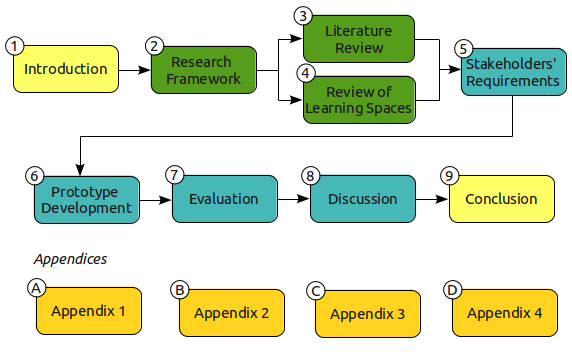
\includegraphics[width=0.9\textwidth]{CH1-F1-Thesis}
\caption{Thesis structure}
\label{fig:ts}
\end{figure}

\begin{description}
\item[Chapter 2.] This chapter presents a methodological approach employed in
this research. Theoretical background of design science research methodology is
given and the way this approach was adopted in this project is described.
\item[Chapter 3.] This chapter focuses on discussing the background of
\LLLsn. Its connection to universities, the current situation in this area and
the problems associated with \LLLs in universities are shown here.
\item[Chapter 4.] This chapter explores the technical worlds of learning
support. System that are currently employed at universities are examined according
to their compliance with \LLLs support.
\item[Chapter 5.] The results of literature review (Chapter 3) and a review of
learning spaces (Chapter 4) are taken to the stakeholders for analysis of their
needs and requirements. Later these findings are used in development of a
conceptual model of an environment that can provide support for \LLLsn.
\item[Chapter 6.] A prototype implementation (based on the requirements
developed in Chapter 5) process and outcomes are presented in this chapter.
\item[Chapter 7.] This chapter describes a complex evaluation design used in the
research to address the questions of quality, functionality and suitability of
the developed features.
\item[Chapter 8.] In this chapter the results and lessons learnt are discussed
with an attempt to analyse issues and question the outcomes. Technical
considerations and practical applications of this research are presented.
\item[Chapter 9.] This chapter brings conclusions and contributions of the
research presented in this thesis. It explores implications for theory and
practice as well as the potential for future research.
\end{description}

This thesis also includes a number of appendices, namely:

\begin{description}
\item[Appendix A] provides ethics documentation for the first stage of the
requirements analysis.
\item[Appendix B] gives an overview of the documents used in the stakeholders
interviews, such as questions used in the interviews and scenarios discussed
with the participants.
\item[Appendix C] consists of the formal requirements specification used for
development of the prototype features. This specification is developed in the
form of user stories.
\item[Appendix D] includes interface screenshots of the prototype features. 
\item[Appendix E] provides ethics documentation for the evaluation stage of this
research project.
\item[Appendix F] overviews the documents used in evaluation Study Two (group
experiment) which includes study protocol, background and exit questionnaire,
participants' responses and the examples of their work.
\item[Appendix G] overviews the documents used in evaluation Study Three (case
studies) which includes study protocol, background questionnaire, and interview
questions.
\end{description}
\chapter{Research Framework\label{cha:method}}
%3100
The main purpose of this chapter is to describe a research approach used in this
study. The first section of the chapter identifies the objectives that need to
be addressed in order to achieve the goal of this study, followed by the research
questions in Section \ref{sec:questions} raised from these objectives.

Design Science Research (DSR) methodology was adopted by this study as the main
research methodology to address the research questions. This methodology
emphasizes the problem-solving and performance-improving paradigms and is
oriented towards creating and evaluating IT artifacts \citep{Hevner2004}. A
five-stage research project framework is outlined in Section \ref{sec:method}
which explains each stage of the project and the methods applied. Methodological
limitations are brought to considerations in Section \ref{sec:limits}. This
chapter concludes with the discussion of related work and projects carried out
in the area of \LLLsn.

\section{Research Objectives}

Understanding how \LLLs in universities can be effectively supported using
technical solutions is an overarching goal of this research. This goal brings up
a number of objectives that need to be addressed:
\begin{description}
  \item[Objective 1.] To determine student and institutional requirements for a
  \LLLs environment within the university context.
  \item[Objective 2.] To identify shortcomings and map these requirements
  against the systems already used in universities to support \LLLsn.
  \item[Objective 3.] To design and implement the features required in an
  environment that supports \LLLs to satisfy the defined requirements.
  \item[Objective 4.] To evaluate how this environment meets the needs of all
  stakeholders in supporting \LLLsn.
\end{description}

\section{Research Questions}
\label{sec:questions}
Based on the objectives, this study addressed the following research questions
supported by sub-questions:

\begin{description}
  \item[RQ1:] \textit{What is the concept of \LLLs and its connection to 
  universities?}
	\begin{itemize}
	  \item What is the role of \LLLs in the university context?
	  \item What is the motivation of universities in supporting \LLLsn?
  	  \item What are the existing university policies for supporting \LLLsn?
      \item What are the components of \LLLs environments in universities?
      \item What are the requirements for successful \LLLs support in
   universities?
	\end{itemize} 
	
   \item[RQ2:] \textit{How are available e-tools used to support \LLLs within
   the university context?}
	\begin{itemize}
		\item What e-tools are currently available to support \LLLsn:
			\begin{itemize}
				\item in general?
				\item in universities?
			\end{itemize}
		\item What are the conceptual strengths and weaknesses of these e-tools in
		university context?
		\item What is the relationship between LMS and e-tools support for \LLLs in
		university context?
	\end{itemize}

	\item[RQ3:] \textit{How can LMS and/or \ep~systems be extended to support
	students in the university context for \LLLsn?}
	\begin{itemize}
		\item What features are available now in these systems?
		\item What are the students and institutional requirements for LMS and
		\ep~to support \LLLsn?
		\item How can these requirements be translated and implemented into new or
		improved features?
	\end{itemize}

	\item[RQ4:] \textit{How does this extended environment meet the needs of 
	stakeholders in university teaching and learning contexts?}
	\begin{itemize}
		\item How can lecturers use new features to provide students with their
		guidance and help them to understand \LLLs skills?
		\item How can students address \LLLs skills using new features?
		\item How can new features help students track their learning progress, manage
		\ep~knowledge and content, demonstrate and share their achievements with
		others?
	\end{itemize}
\end{description}

\section{Research Approach}
\label{sec:method}

Finding the most efficient research approach is an important part of any
research study. A properly selected approach helps to obtain answers to the
research questions while working within the framework that uses methods that
have been verified and tested for validity \citep{Kumar2005}. Multi-paradigmatic
field of ICT offers a number of methodologies (e.g., theory building and
testing, action research, interpretive research, grounded theory, etc.) drawn
from the variety of research philosophies \citep{Vaishnavi2007}. This study
follows design science research methodology that has become popular over the
last five decades as fundamentally a problem-solving approach \citep{Cross1993}.

\subsection{Design Science Research Methodology}

According to \citet{Peffers2008}, design science research (DSR) originates from
engineering and computer science where design is a component of the research
process. \citet[p.~4]{Iivari2009} define DSR as \inlinequote{a research
activity that invents or builds new, innovative artifacts for solving problems
or achieving improvements}. Unlike software development methodology that
does not necessarily need any underlying theory, design science requires a
theoretical foundation for research \citep{Gero1999}. This approach is used in
ICT where there is a need to extend the existing boundaries of the current
systems or to address the important problems by creating new solutions and
artifacts \citep{Hevner2004}. The artifacts can be described as constructs
(vocabulary of a domain), methods (algorithms), models (abstractions),
instantiations (prototype systems), and better theories \citep{Hevner2010}. 

Requirements for DSR project contribution, defined by \citet{March2008}, include
(1) identification of a problem, (2) demonstration that there are no existing
adequate solutions in the area, (3) development of an innovative artifact that
addresses the problem, (4) evaluation of the artifact, (5) communication of the
knowledge added to the area, and (6) understanding of the implications for
theory and practice.

This set of requirements closely resembles the DRS methodology process described
by \citet{Peffers2008} (see Figure \ref{fig:peffers}) and research model phases
found in \citet{Vaishnavi2007} (see Figure \ref{fig:vaishnavi}).

\begin{figure}[h!]
\centering
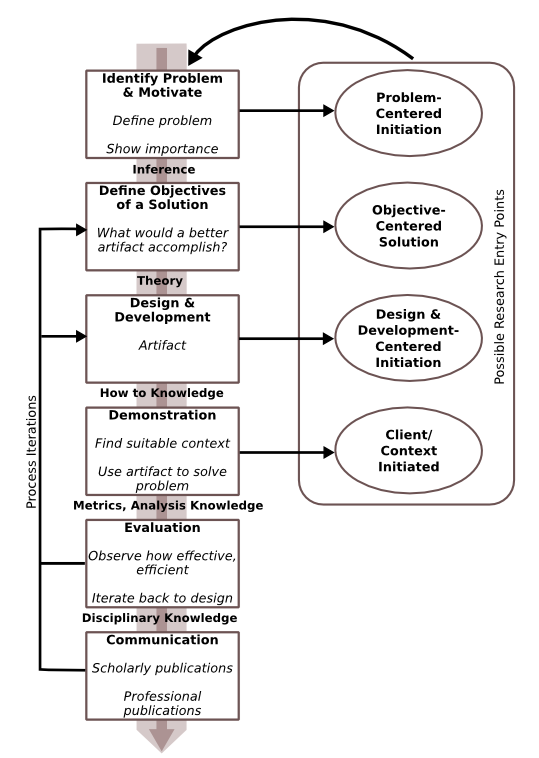
\includegraphics[height=0.76\textheight]{CH2-F1-Peffers}
\caption[Design Science Research Methodology Process Model]{Design Science
Research Methodology Process Model \citep{Peffers2008}}
\label{fig:peffers}
\end{figure}

\FloatBarrier

\begin{figure}[htp]
\centering
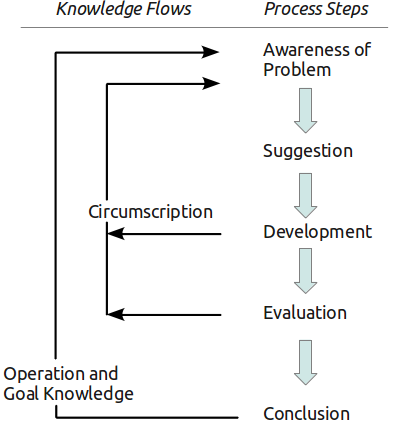
\includegraphics[width=0.5\textwidth]{CH2-F2-Vaishnavi}
\caption[Design Science Reseach Cycle]{Design Science Research Cycle
\citep{Vaishnavi2007}}
\label{fig:vaishnavi}
\end{figure}

All authors essentially agree on common elements. The initial stage of research
is \textit{problem identification} or \textit{awareness}, where a specific
research problem should be stated and the importance of its solution should be
justified. After the problem is identified, the next step is to \textit{suggest
a solution} and define its objectives. This includes understanding the state of
the problem and current available solutions, if any, and explaining how new
solution is going to address the problem in a better way. 

\FloatBarrier

The core phase of research is \textit{design and development}. Conceptually,
this phase consists of deciding the artifact's functional requirements or its
architecture and afterwards creating artifact itself. \citet{Peffers2008} note
that in some cases an artifact is not necessarily a new development. It might
have been already used in another research domain to solve a different problem.

Unlike Vaishnavi's research cycle where evaluation is one step of research
process, Peffer's model distinguishes between \textit{demonstration} and
\textit{evaluation} of the artifact. Demonstration is used to show that the
implemented idea works, while evaluation is a more formal form of measurement of
how well the artifact supports a solution to the problem \citep{Peffers2008}.
Artifact can be evaluated from various perspectives such as performance,
usability, reliability, accuracy, quality, functionality, etc.

The last stage of research is \textit{conclusion} or \textit{communication}. It
might involve but is not limited to: discussing the problem, its importance, the
novel artifact, and its effectiveness with relevant research audiences; creating
scholarly publications; presenting research findings at the conferences; and
writing a project report \citep{Archer1984}. However, if no satisfying results
have been reached at this stage of the research cycle, it might as well serve as
a subject for further research.

Described in Table \ref{tab:guidelines} are seven guidelines identified by
Hevner \citeyearpar{Hevner2004} that should be followed by the beginning
researches for effective DSR.

\begin{table}[htb]
  \caption[Design Science Research Guidelines]{Design Science Research
  Guidelines \citep{Hevner2004}}
  \begin{center}
    \begin{tabular}{| l | p{6.5cm} |}
    \hline
     \multicolumn{1}{|c|}{\textbf{Guidelines}} &
     \multicolumn{1}{c|}{\textbf{Description}} \\
     \hline
     Guideline 1: Design as an Artifact & Research must produce a viable
    artifact such as a construct, a model, a method or an instantiation \\ \hline
     Guideline 2: Problem Relevance & Research must develop technology-based
     solutions to important and relevant problems \\ \hline 
     Guideline 3: Design Evaluation & Proper valuation methods must be used to
     demonstrate artifact's quality and efficacy \\ \hline 
     Guideline 4: Research Contributions & Research must provide clear
     contributions to the research areas \\ \hline 
     Guideline 5: Research Rigor & Rigorous methods must be applied to
     construction and evaluation of the artifacts \\ \hline 
     Guideline 6: Design as a Search Process & Research must incorporate a
     search process to find and effective solution to the problem \\ \hline
     Guideline 7: Communication of Research & Research must be effectively
     communicated to relevant audiences \\ \hline
    \end{tabular}
  \end{center}
  \label{tab:guidelines}
\end{table}

In contrast to Hevner, \citet{Venable2010} argues that there is no common
understanding of what kind of guidelines and standards should be used for
effective DSR. However, based on analysis in the same work, the majority of
respondents who are researchers and DSR practitioners agree on a few points: DSR
should address important problems, have an artifact that would help to solve the
problem, and have some kind of evaluation of this artifact.

\subsection{Design Science Research Applied to This Project}

The research framework in the current research is adapted from a DSR cycle
established by \citet{Vaishnavi2007}. They identify five phases in the research
model: (a) identification of a problem, (b) suggestions and objectives of a
solution, (c) design and development, (d) demonstration and evaluation, and (e)
conclusion and communication.

\begin{figure}[htb]
\centering
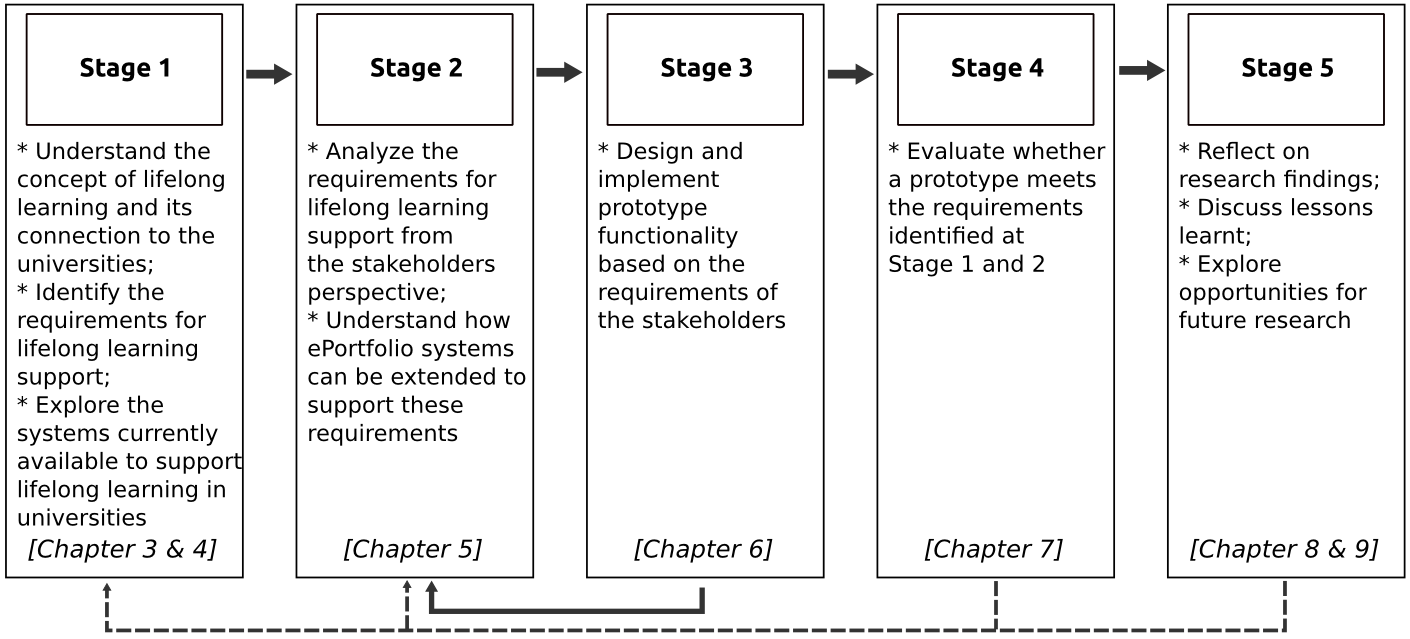
\includegraphics[width=1\textwidth]{CH2-F4-Path}
\caption{The research path}
\label{fig:path}
\end{figure}

Figure \ref{fig:path} shows a research path of this project from the first
to the last stage. It can be seen that at the later stages of the project it was
necessary to look back and reflect on findings in order to understand whether
the research objectives were met and what lessons were learnt. Other iterations
in this project were between stages three and two where the prototype had to be
taken back to the stakeholders for feedback. Although, according to Figures
\ref{fig:peffers} and \ref{fig:vaishnavi} the end of the evaluation can be
considered another potential stage to iterate back, \citet{Peffers2008} says
that the nature of the research project usually shows whether iterating back is
feasible or not. In this case, due to the time and resources constraints,
further improvements were left to the subsequent research projects.

\subsubsection{Stage 1. Problem Identification and Motivation}

Any research project can be started either from the gap in the literature or
when a problem that is worth solving exists \citep{Bourner2002}. Previous
experience and observations of the existing problems in the field of study
formed the background for this research. To define the main research topic,
preliminary investigations were made as part of the field of study review. The
problem identified in the current research is the difficulty in supporting
students' \LLLs in universities. Defining the research topic led to the research
questions and objectives development which, in turn, formed the direction and
focus of this project.

\subsubsection{Stage 2. Objectives of a Solution}

To answer the research question on the concept of \LLLs and what kind of
environment can support it, it is important to develop understanding of
current theories and practices of \LLLs support. A comprehensive literature
review and a review of the learning spaces was undertaken to address these
questions.

However, this research did not rely on a literature review alone. A set of
interviews with the stakeholders were organized to support literature findings
and identify the gaps that exist in current \ep~systems. Interviewees were
asked to look at the \ep~system from the \LLLs perspective and offer their
solutions for supporting guiding principles and recommendations for successful
\LLLs discovered in the literature.

Interviews were audio recorded, transcribed and analyzed. The results were
compiled into a set of formal software requirements specification to be
implemented in a system prototype for the future evaluations.

\subsubsection{Stage 3. Design and Development}

In the development phase, the results of the literature review, interviews and
requirements analysis were used to create a conceptual model of an \ep-supported
environment that can facilitate students in \LLLs and be compatible with
university needs.

A functionality, based on this model, was implemented in a prototype \ep~system.
As the requirements specification was too large for a project of limited size
and within a relatively short timeline, only high priority requirements were
implemented. The requirements were prioritized according to the feedback given
by the interviews participants at the initial stages of the project. Due to
this, a number of requirements related to a better integration of the
\ep~systems with LMS and usability improvements were omitted. Although these
requirements were not implemented, they were still included into the conceptual
model.

Prototyping followed established software engineering practices that interleaved
coding and revision, forming iterative development cycles, as shown in Figure
\ref{fig:prototype}.

\begin{figure}[htb]
\centering
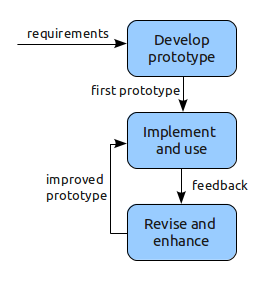
\includegraphics[height=0.3\textheight]{CH2-F3-Prototype}
\caption[Prototyping]{Prototyping based on \citet*[p.~411]{Sommerville2007}}
\label{fig:prototype}
\end{figure}

After each iteration was completed, the prototype was taken back to the
stakeholders for feedback. This was necessary to understand what changes were
required and to design further improvements. These iterations are shown on
Figure \ref{fig:path}.

Mahara \ep~system\footnote{\url{http://mahara.org}} was used as an initial base
system for the prototype. There is a number of reasons why this system was
selected. Mahara is a trusted and widely-used in universities (and at Massey
University in particular) solution with a large community support. This system
is open source which makes it easy to access and allows modifications like
adding new features and changing the existing ones. Mahara is a \textit{typical}
representative of its category and provides all commonly available features. At
the same time it is a leading edge system developed by using latest web
technologies and programming practice.

\subsubsection{Stage 4. Demonstration and Evaluation}

It is important for evaluation to be treated not as an isolated process, but as
a part of design process \citep{Cleven2009}. Although, the prototype was
reviewed by the stakeholders after every development cycle, a formal evaluation
of the overall concept was still required.

It is not likely that a single evaluation technique can establish effectiveness
and value of the prototype in a complex area of \LLLsn. In such cases it is
recommended \citep{Quinlan2008} that the evaluation design should incorporate a
variety of methods, that taken together can provide reasonable evaluation
outcomes.

Due to time and resources constraints, and an extended \ep~system being a
functional prototype, it was not feasible to conduct evaluations in the real
world settings. However, it was possible to develop a number of studies that
looked into the specific aspects of \LLLs support and evaluated how well
developed features satisfy the requirements identified earlier by the
stakeholders.
 
As a result, features implemented in the prototype were evaluated from three
different perspectives: 

\begin{itemize}
  \item Demonstrations of the prototype and its extended functionality were used
  for exploratory evaluation with the lecturers. The aim was to explore how the
  lecturers can integrate new features into their teaching to provide students
  with guidance and help them to understand \LLLs skills.
  
  \item An experiment with various representatives of undergraduate students
  was undertaken to understand how added functionality can help them to address
  institutional graduate attributes and \LLLs skills. Thirty five students with
  different levels of knowledge of \LLLs skills and experience of using
  \ep~systems were involved in the experiment.

  \item Case studies were used to evaluate the prototype from the mature
  students' perspective. This approach was selected due to its internal and
  external validity, control and in-depth examination of each case \citep{Yin2009}.
  Participants with different study backgrounds had access to the prototype for
  an extended trial period of time and were able to get a better look at the new
  features. At the end of the trial period, each participant was interviewed and
  gave their feedback on the features they had used.
\end{itemize}

\subsubsection{Stage 5. Conclusion and Communication}

Where it was possible the results of the various stages of this research project
were documented and submitted for publications and conference presentations. A
full list of publications can be found in \hyperref[sec:pub]{Publications and
Presentations} section of this thesis.

\section{Methodological Limitations}
\label{sec:limits}

Any study and its findings should be weighed against methodological
limitations. Acknowledging limitations is important for scientific progress as
they might help to understand how research can be improved in the future
\citep{Ioannidis2007}. Although, literature does not explicitly describe
limitations of DSR methodology, they can still be derived from the limitations
of the methods used at each stage of the study. Therefore, the limitations
considered in this research included:

\begin{description}
\item[Sample size:] Sample size for Stage 2 was relatively small due to the
participants profile requirements. In addition, the snowballing sampling
technique was used to find suitable student participants which might have
influences the outcomes of this stage.
\item[Prototyping:] The evaluated system was a prototype based on the open
source \ep~system Mahara which might have led to biased feedback as some
participants were familiar with the system and already had their opinions about
it.
\item[Evaluation:] Due to the nature and scale of this research project, its
time and resources constraints, evaluation was not conducted in real world
settings. Alternatively, a set of case studies, an experiment and exploratory
evaluations have been undertaken.
\end{description}

A more detailed discussion of the limitations can be found further in the
relevant chapters of this thesis.

\section{Related Work}
\label{sec:related}
As \LLLs concepts gained general acceptance, there were a number of studies
aimed to explore \LLLs support in various contexts. To date, research similar to
this project has not been identified, although projects found were a valuable
source of information and examples of previous research experience.

\begin{itemize}
  \item Lifelong Learning in London for
  All\footnote{\url{http://www.lkl.ac.uk/research/l4all.html}} (L4All): This
  project is focused on developing of \LLLs system to support independent
  learners (particularly those 16+ learners who traditionally have not
  participated in higher education) by recording their learning pathways. This
  project aimed to provide lifelong learners in the London region with access to
  information and resources that facilitates their progression from secondary
  education to further education or from secondary education directly to higher
  education \citep{Freitas2006};

  \item The Regional Interoperability Project on Progression for Lifelong
  Learning\footnote{\url{http://www.nottingham.ac.uk/rippll}} (RIPPLL): This
  project was going to establish a model of cross-sector collaboration in
  personal development planning technology in the UK. The aim was to make all
  the major existing electronic systems interoperable for study-based progress
  files that are used in further and higher education to provide an easier
  transition process from school to further education \citep{Hartnell-Young2006};

  \item ELGG-Moodle: In autumn 2006 Klagenfurt University, Austria was piloting
  the project that aimed to integrate Moodle LMS and ELGG platform. This
  integration was used for professional development for all academic staff.
  Project outcomes provided integration between systems such as single login and
  file transfer \citep{Attwell2007}.

  \item Accessible \LLLc for Higher
  Education\footnote{\url{http://www.eu4all-project.eu}} (EU4ALL): A project
  started in 2006 that aimed to develop components and services for universities
  to make learning more accessible for both the students with functional
  diversity and the elderly. This project looked into providing better access
  to the electronic content and educational resources in higher education using
  a framework or a set of free tools that support mobile learning, audio
  recording transcription, DAISY digital books and other adaptations of contents
  based on the student's needs and preferences.

  \item An \ep~based Pedagogy for Small to Medium-sized
  Enterprises\footnote{\url{http://www.wlv.ac.uk/ePPSME}} (ePPSME): Finished
  in 2011, this project provided higher education sector with reusable models
  for an \ep-based pedagogy for work-based learners. This pedagogy addresses
  the needs of learners with shortage of time, previous informal learning
  experience, need for flexible delivery and quality of learning, and
  opportunities to record achievements \citep{Felce2011}.
\end{itemize}

Unlike this research, the majority of above described project were focusing
either on collaboration between sectors (school -- university or university --
workplace) or were aimed at developing of theoretical rather than practical
solutions. The ELGG-Moodle integration project was the most relevant in
the technical context of this research, however it focused on not students,
but staff development. 

As well, these project were analysed with the intention of adopting a suitable
evaluation design. However, an approach feasible for the research of this size
and timeframe has not been found among the previous projects.

\section{Summary}

To address the objectives and research questions stated at the beginning of the
chapter, this research project follows DSR methodology. DSR is a problem solving
approach that focuses on development and evaluation of innovative IT artifacts.
This chapter outlined a five-stage research framework used in this work with
each stage explained.

The next chapter will explore the literature review undertaken to understand the
concept of \LLLs and the requirements for its efficient support. It will provide
a background for the further theory development of this research.
 
\chapter{Literature Review - Lifelong Learning \label{cha:litrev}}

In order to answer the first research question, it is important to establish a
basic understanding of the main concepts used in this work. Although,
underlying concepts can be found primarily in the domain of education, they make
a good starting point for a discussion. 

This chapter introduces the key concept of \LLLs that will be in focus
throughout the thesis. First, the origins of the term of ``\LLLsn'' and related
concepts are discussed in Section \ref{sec:concepts}. The crucial differences
between these concepts and how they transformed over time, driven by changing society and
economics, are explored. Second, through the increasing focus on \LLLs skills in
the world of work and in higher education, Section \ref{sec:uni} shows the need
for \LLLs support in universities. Universities are in center of this
dicussion as they provide the necessary organizational framework, theoretical
principles and practical experience for \LLLs \citep{Knapper2000}, which can be
seen in the role and influence of the universities in the educational systems of
most countries as the ``keepers of the intellectual traditions of a nation"
\citep[p.~96]{Longworth2003}. Third, in Section \ref{sec:needs} the general
needs for successful \LLLs are outlined. No explicit requirements have been
found in the literature. However, commonly accepted recommendations and
guidelines were discovered in various sources that will be used as a background
for further exploration in Chapter \ref{cha:model}.

\section{Literature Review Process}
The literature review on \LLLs (Chapter \ref{cha:litrev}) and a review of
institutional and open learning spaces (Chapter \ref{cha:systudy}) that provide
and support background for this thesis were conducted by systematically reading
and reviewing books, journals and conference proceedings in the area of
research. The main methods to identify relevant literature were recommendations
of domain experts and a library search. Relevant articles were identified by
reading titles and abstracts of selected journal articles and papers in
conference proceedings. Where possible the latest ten years of issues of the
following journals were looked through: ``British Journal of Educational
Technology'', ``International Journal of Lifelong Education'', ``European
Journal of Education'', ``\LLLc in Europe'', ``International Journal of Emerging
Technologies in Learning'', ``New Zealand Journal of Adult Learning'', ``Journal
of Computer Assisted Learning'', ``European Journal of Engineering Education'',
and ``International Journal of ePortfolio''. In addition, a keyword search was
carried out on the Internet and academic resources (such as Education Research
Complete\footnote{\url{http://www.ebscohost.com/academic/education-research-complete}},
Academic Search
Premier\footnote{\url{http://www.ebscohost.com/academic/academic-search-premier}},
Directory of Open Access Journals\footnote{\url{http://www.doaj.org}},
Google\footnote{\url{http://google.com}}, Google
Scholar\footnote{\url{http://scholar.google.com}}) to cover conference
publications not available in the library. The following keywords and
combinations of keywords were used in the search: ``\LLLsn'', ``life-long
learning'', ``e-learning'', ``ePortfolio'', ``e-portfolio'', ``electronic
portfolio'', ``Web 2.0'', ``learning environment'', and ``learning
technology''.

This review helped to discover previous work in the area (described in Section
\ref{sec:related}), explore methods that could be applied to this research,
increase the depth and breadth of knowledge of the field, and identify domain
experts and other people working in the same field who could be valuable to
contact. Besides finding relevant information in the literature, it was also
notable to identify the gaps that currently exist (more detailed discussion can
be found in Chapter \ref{cha:systudy}). It will be shown further that these gaps
are based on facts that although a lot of work has been done on developing \LLLs
theories as well as developing technologies for education and learning, there is
little substantial work done on combining these two areas.

As a continuous process, the literature review for this research was updated by
actively acquiring and reading the relevant articles emerging in the literature.

\section{The General Concept of \LLLc}
\label{sec:concepts}
\subsection{Terms and Definitions}

The European Commission \citeyearpar{EuropeanCommission2000} defined \LLLs as:

\longquote{All learning activity undertaken throughout life, with the aim of
improving knowledge, skills and competencies within a personal, civic, social
and/or employment-related perspective.} 

However, it is not as simple as it looks: the concept of \LLLs consists of a
variety of meanings, models and ideas. Such terms as '\LLLsn', 'lifelong
education', 'adult education', 'recurrent education', 'continuing education',
and 'further education' create a set of to some extent related, yet different
concepts \citep{Hager2011}.

'Continuing education' (also referred to as 'adult education') was introduced in
the late 1970s and early 1980s. There was no common definition of this term,
but in some sources  \citep{Jarvis2004} it was described as all learning
activities which could be undertaken after compulsory schooling is finished.
Figure \ref{fig:learning} compares the main concepts in education according to
the time spent by individuals learning/studying across their lifespan. As can be
seen, continuing education was usually part-time and accured less frequesntly
than other forms of education.

\begin{figure}[htb]
\centering
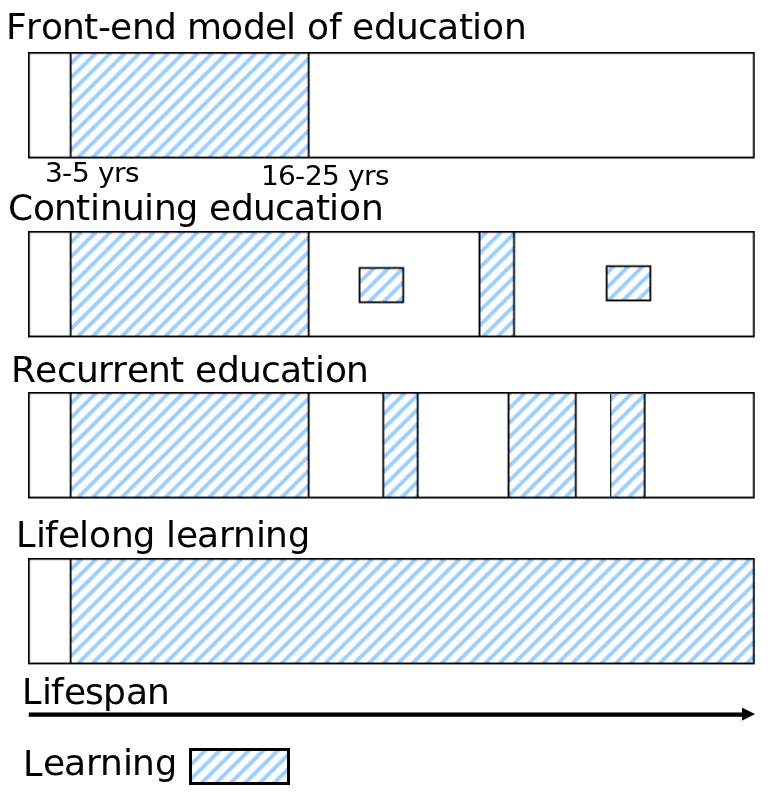
\includegraphics[width=0.55\textwidth]{CH3-F1-Learning}
\caption[Changing concepts of learning]{Changing concepts of learning 
\citep{Jarvis2004}}
\label{fig:learning}
\end{figure}

The term 'recurrent education' was widely used by OECD until the 1980s
\citep{Jarvis2004}. Unlike intermittent continuing education, its idea was
in allowing adults to spent full time studying in formal education sector doing
on-the-job trainings or post-compulsory education of any kind. Arguably, this
main feature of the right for full time study made the concept of recurrent
education disappear from the governments' eduactional agendas: it was too
expensive and difficult to support this policy.

Rejecting the concepts of recurrent and continuing education played an important
role in development of the new educational models. While they had different
undelying  philisophy, they both recognized the fact that aquisition of
knowledge should be a lifelong process, from ``cradle to grave''
\citep{Hargreaves2004}.

The origin of the term '\LLLsn' goes back to the early 20th century and is
contributed to by John Dewey \citeyearpar{Dewey2004}. From his perspective,
\LLLs had to be centered on the individual's ability to take an active role in
democratic society. He saw education as a learning process which was influenced
by the growth of the individual and society, both interlinked. Dewey's key to
\LLLs was in developing active learning, enabling the individual to reflect and
change throughout life, emphasizing that non-formal education was as important
as formal education.

The concept of 'lifelong education' was discovered in 1972 after Edgar Faure's
Report ``Learning to Be'' for UNESCO. The concept described in the report was
announced to be the leading one for the reform in education. Faure's Report used
four principles for the lifelong education architecture \citep{Faure1972}:
vertical integration (education should occur throughout one's life), horizontal
integration (acceptance of non-formal and formal education), the democratization
of education (more widespread involvement of learners) and learning society
(restructuring of educational system). However, according to Hager's
\citeyearpar{Hager2011} analysis, UNESCO's concept of 'lifelong education' put
the emphasis on formal education as the only sufficient and relevant form of
learning to provide actual 'education'.

\subsection{Paradigm Shift and \LLLc Today}

Almost 40 years after the idea of this lifelong education was introduced, many
governments rediscover not lifelong education, but \LLLs \citep{Boshier2000}.
This shift was not only semantic, but also substantive, which showed that \LLLs
and lifelong education are not the same: lifelong education aimed to develop
more humane individuals and communities, while \LLLsn's goal was in retaining
and gaining new skills that would help individuals adapt to rapid changes in
their workplace \citep{Medel-Anonuevo2001}. Lifelong learning is based on the
notion of the individual learner as a consumer. And as a result if consumers
decide not to take advantage of all the opportunities they have -- then it is
their fault. Therefore, being constructed as individual activity, learning
depends entirely on personal motivation. Unlike learning, education is a
provided service \citep{Boshier2000} that requires someone to be responsible for
providing resources, developing policies, etc. The emphasis on 'learning' rather
than 'education' is significant \citep{Tuijnman2002}, as it moves focus from the
institutions onto the individual. Although, it does not mean that institutions
and govermnets play no role whatsoever. Their role is rather transformed into
investment in individuals and creation conditions for them to take charge of
their learning \citep{Chen2009}.

Over the last decade, lifelong learning support has become a part of official
government policy in a number of countries around the world. As an example,
European Commission has established a budget of nearly 7 billion Euro for the
period of 2007-2013 for 'Lifelong learning programme' which aims to support
education and training at school, college, university, in the workplace and in
the community across Europe \citep{TheEducation2009}. In New Zealand a number of
governmental documents \citep{NewZealandMinistryofEducation2008} now mention
the ``success of all New Zealanders through lifelong learning". As a result, the
national tertiary education system of the country has been transformed to
support lifelong learning ideals \citep{Benseman2006}.

\begin{figure}[htb]
\centering
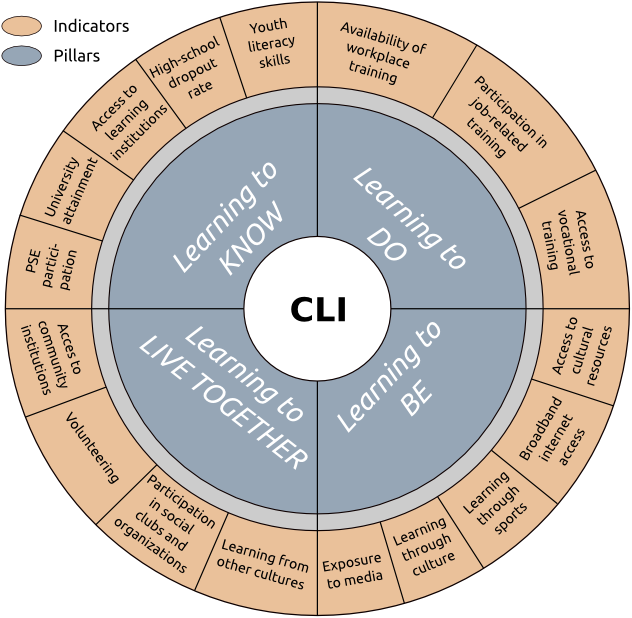
\includegraphics[width=0.8\textwidth]{CH3-F2-CLI}
\caption[The 2010 Composite Learning Index of Canada]{The 2010 Composite
Learning Index of Canada}
\label{fig:cli2010}
\end{figure}

In 2006 Canadian Council on Learning developed the 17 indicators and 26
specific measures (Figure \ref{fig:cli2010}) called Composite Learning Index
(CLI) that is used to calculate annual progress in \LLLs in the country
\citep{CanadianCouncilonLearning2011}. Using CLI, Canadian government expects to
draw attention to the benefits of \LLLs and demostrate learning opportunities
that occur outside of classroom settings. In August 2010 European Union adopted
this Index as European \LLLc Indicators (ELLI). Similar to CLI, ELLI were using
UNESCO approach of four pillars of learning: Learning to Know, Learning to Do,
Learning to Be, and Learning to Live Together \citep{ELLIDevelopmentTeam2010}.

\subsection{Components and Attributes of Lifelong Learning}
In terms of purposeful learning activities \LLLs consists of the following
components \citep{Longworth2003, Tuijnman2002}:

\begin{itemize}
  \item Formal learning -- institutionally graded, and hierarchically structured
system, often leads to qualification;
  \item Non-formal learning -- organized systematic educational activity
  external to formal education;
  \item Informal learning -- planned or not planned, but conscious learning from
the experience;
  \item Incidental learning -- not intentional, an accompaniment to everyday
  life, learning during the action.
\end{itemize} 

\begin{figure}[htb]
\centering
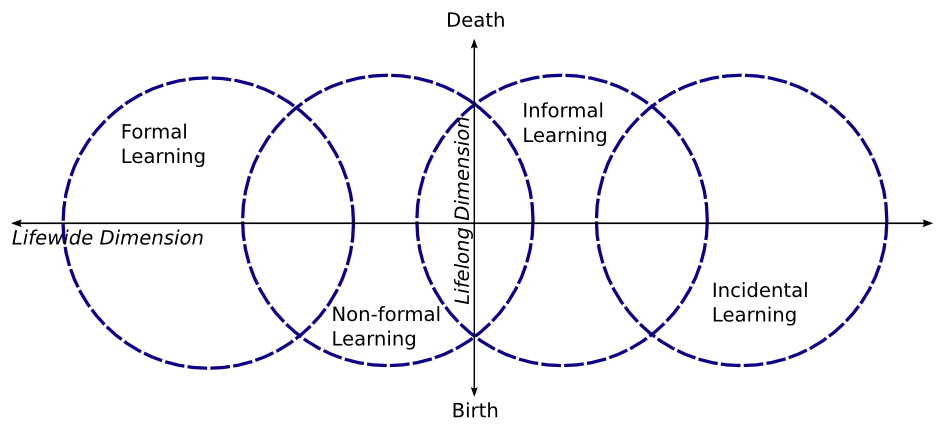
\includegraphics[width=0.8\textwidth]{CH3-F3-LLLFramework}
\caption[Framework for \LLLc]{Framework for \LLLc (based on
\citet[p.~11]{Divjak2004})}
\label{fig:lllfmwrk}
\end{figure}

Some researchers \citep{Longworth2003} recognize only two categories of lifelong
learning, formal and non-formal, leaving informal and incidental parts of it as
the elements of non-formal learning. Boshier \citeyearpar{Boshier2000} states
that the current reality is such that the formal and non-formal categories of
\LLLs are like ``two parallel railway lines. Both cross the landscape but never
touch'' (p. 11), explaining this way that formal setting have practically
nothing to do with non-formal.

From another perspective, \LLLs encompasses the elements of self-direction,
long-term and life-wide learning \citep{Schuetze2006}. Rubenson
\citeyearpar{Rubenson2002} called these 'three fundamental attributes of \LLLs':

\begin{itemize}
  \item Lifelong -- means everything from cradle to grave;
  \item Life-wide -- takes place outside the formal education system;
  \item Self-directed -- is guided by the learners themselves and does not
  limit itself to education.
\end{itemize} 

Weert and Kendall \citeyearpar{Kendall2004} gathered other essential
characteristics of \LLLsn:

\begin{itemize}
  \item Most of \LLLs occurs outside of classroom as is not triggered by
  textbooks;
  \item The driving force in \LLLs is self-motivation and active participation
  of learners;
  \item Lifelong learning involves interactions, groups, community learning and
  other social activities;
  \item Solving atrificial tasks does not matter in \LLLsn. Achievements in
  real-life situations measured by common standards are important;
  \item Lifelong learning is learner centred and aims for personal
  achievements;
  \item Lifelong learners should maintain their achievements portfolio.
\end{itemize} 

These characteristics describe \LLLs as demand-driven, flexible, social and
personal at the same time. Hereinafter, any further reference to \LLLs will be
made in terms of the concepts outlined in this section.

\section[\LLLc in Universities]{\LLLc in Universities\footnote{This section was
adopted from the section originally published as part of Chapter 8 ``The Role of
Institutions in Creating Student-Focused Virtual Learning Spaces with ePortfolio
Systems'' of the book ``Physical and Virtual Learning Spaces in Higher
Education: Concepts for the Modern Learning Environment". Full reference can be
found in Publications section.} }

\label{sec:uni}

As \LLLs consists of the concepts of 'life-long', 'life-wide' and 'self-
directed' learning, it has following significant implications. As already
mentioned above, 'life-long' means the full life span of an individual. From the
institutional view it starts when students are enrolled in the university and
finishes when they graduate. 'Life-wide' component of learning implies that
learning can and should occur not only as formal university study, as personal
and professional development takes place in many contexts. Attwell
\citeyearpar{Attwell2007} considers the fact that everyday non-formal types of
learning are not connected to institutional formal education to be the major
issue of modern learning, which can make students see their study at university
as ``something irrelevant to their identities'' (p. 4). For successful \LLLs,
progress of the achievements should be recorded and maintained over a long
period and across various sources, formal as well as non-formal \citep{Kay2008}.
A \LLLs environment needs to acknowledge this and allow learners to record and
reflect on experiences from all these contexts.

Over recent years the skills that provide \LLLs ability were identified, they
include: solving problems, critical thinking, utilizing technology, and
information literacy; working with others in teams, communication skills,
leadership and social interaction skills; self-management; collecting, analyzing
and organizing information; planning and organizing activities; cultural
awareness and understanding
\citep{Brooks2008,Heinrich2007,Otala1997,Pitman2009}. The importance of these
skills in addition to academic and subject knowledge has been increasingly
emphasized in the workplace and public policy
\citep{Morgan-Klein2007,Sutherland2006}. Individuals today need to continue to
update and upgrade their skills and knowledge even after completing formal
education in order to survive in the changing world. Otala
\citeyearpar{Otala1997} states that required flexibility and adaptability to
these rapid changes are gained through ``better developed learning skills and
the right attitudes that help individuals quickly and easily learn new things''
(p. 456). Therefore, current students need to ``possess something more than
skills which grow obsolete as technology advances'' \cite[p.~195]{Field2003}. 

Higher education institutions have responded to the need for \LLLs skills by
defining their own strategies to promote \LLLsn. Many institutions in Europe,
the United States, Australia and New Zealand now explicitly express the \LLLs
characteristics they strive for in their graduates \citep{Scanlon2006}.
Australian universities, such as Curtin University, have made policy
declarations committing to graduate attributes across their programmes
\citep{CurtinUniversity2006}. The College of Sciences of Massey University has
formulated a draft \LLLs policy \citep{MasseyUniversity2008} that expresses
values, support and expectations in regards to \LLLsn. Graduate profiles, naming
\LLLs skills such as critical thinking, effective communication, teamwork and
leadership have been established for many degree programme
\citep{Davies2003,McAlister2003}. The accreditation criteria for engineering
degrees now refer to and demand soft skills \citep{Aller2005,Muffo2001}. The
need for a holistic education and the development of students beyond technical
competency is requested \citep{Brakke2002,Davies2003,Dowling2006,Fallows2003,Grabowski2004,Hernon2006}.

In order to enact policy academics need to incorporate development opportunities
for these skills into their teaching and learning designs. While individual
academics succeed in doing so by using techniques such as group work, reflective
journals and authentic assessment \citep{Clarke2003,Lombardi2008}, universities
are far from achieving the required levels of \LLLs skills in their graduates
for the following reasons.

While graduate profiles express graduate attributes and \LLLs skills, the
individual courses making up the degrees have not been adjusted accordingly. One
consequence of this is that students are not presented with a coherent picture
across their courses and that it is too easy to disregard the messages given in
single courses. Some academics may lack awareness, skills and support to fully
incorporate the development of \LLLs skills into their teaching. Academics who
do not consciously practice their own \LLLs skills development will find it
difficult to lead and to inspire their students. Yet, students need guidance in
developing \LLLs skills \citep{Leone2019}, both to recognise their importance
and to acquire the knowledge 'how to' study \citep{Medel-Anonuevo2001}. The
currently dominant academic systems are in conflict with the characteristics of
\LLLs skills. Instead of supporting the needs of learning to be self-directed,
life-wide and lifelong, these systems are assessment-driven and focus on course
content and duration.

\section{Requirements for Successful \LLLc}
\label{sec:needs}
Based on considerations outlined earlier in this chapter, this section brings
together the requirements for provision of successful \LLLs support for
students. Although, no explicit set of requirements has been found, the
literature identifies a number of guidelines and recommendations that have to be
satisfied in order to achieve successful \LLLs support in universities. Some of
them have already been mentioned throughout this chapter.
 
\begin{itemize}
  \item Universities should provide support for all aspects of \LLLs (formal,
  informal, non-formal, incidental); 
  \item Students need guidance on various levels \citep{Leone2019};
  \item Lecturer should be an active facilitator and promote involving learning
experiences \citep{Leone2019}; 
  \item Learning materials should be organized in the way that would help
students learn how they learn \citep{Medel-Anonuevo2001};
  \item Communication and collaboration are essential parts of learning process
  \citep{Schaffert2008};
  \item Learning progress should be recorded from various sources and maintained
  over a long period of time \citep{Kay2008};
  \item Students need to be aware of their personal achievements
\citep{Schuetze2006};
  \item Students should develop understanding and confidence in their knowledge
  and be able to address higher-order skills (graduate attributes in university
  context) \citep{Hart1999};
  \item Students should be able to evaluate and reflect on their own performance
and learning progress \citep{Mourtos2003}.
\end{itemize} 

These theoretical recommendations will be used to guide further exploration of
 how \LLLs can be supported using thechical solutions available in universities.

\section{Summary} 

Following from the discussions in this chapter, it is important to emphasize
the next key points: \LLLs plays an important role in current global economics
and society; \LLLs skills have become a fundamental part of personal
development; governments and educational institutions, universities in
particular, are attempting to promote and support \LLLsn; at this stage, \LLLs
support provided in universities is not sufficient to satisfy the needs of
students as lifelong learners.

In order to support this argument, the next chapter will review the world of
learning spaces that are currently used in universities and outside of
educational sector to support various learning activities. The connection and
gap that exists between these systems from the \LLLs prespective will be
thoroughly explored.

\chapter{Review of Institutional and Open Learning Spaces \label{cha:systudy}}
%8250
In the previous chapter it was shown that many factors need to combine to fully
support lifelong learning at universities: changes in the way of thinking of
both students and lecturers, support at the department or institutional levels,
provision of training for staff, and personal motivation of learners. This
chapter looks at \LLLs support from another angle, specifically technical
support. It reviews the area of technology and systems available for supporting
various aspects of learning, and examines how availability of a suitable virtual
learning environment may provide the \LLLs support required by students in
universities.

There are several terms that need to be clarified when discussing virtual
systems, spaces or environments. In this chapter, in order to have a common
understanding of these terms, they will have the following meaning unless
specified otherwise:

\begin{description}
	\item[Open systems:] the systems which provide users with open access and allow
	them to contribute, manage, organize, edit, use, re-use, mashup, create or
	alter content of the system \citep{Fay2009}. Such systems might even allow to
	make changes to the actual programming code of the system. Examples of the open
	systems might include Wordpress, Blogger, MediaWiki, Unix, or to some extent
	Facebook and YouTube.
	\item[Closed systems:] the systems which allow users to use content as is, with
	minimal modification to the actual system or program \citep{Fay2009}. Such
	systems are usually proprietary or have a proprietary format of content. Access
	to the closed systems is can be restricted. Examples of closed systems
	might include electronic library catalogues, online banking systems, or
	conference proceedings database.
\end{description}

The virtual learning spaces of universities are dominated by Learning Management
Systems (LMS) supporting course-related work. LMS have been started as and
still are often closed systems that require user accounts and access permissions
to the learning space. These closed systems contrast to open learning spaces
provided by Web 2.0, and social networking tools in particular, which are
characterised by open access allowing individuals to participate under their own
direction in contributing information. Social networking includes sharing,
exchanging and reflecting which provides benefits for learning. 
 
To understand the barriers and issues of utilising closed and open learning
spaces within the university environment, this chapter first explores the
currently dominant LMS and then contrasts them with the Web 2.0 virtual social
spaces. Finally, it introduces an \ep~and \ep~systems as a potential solution
that can help to close the gap that exists between the institutional and
personal learning environments. \ep~characteristics as well as the strengths and
weaknesses of selected \ep~systems are reviewed. A possible way of mapping of
the features these systems provide against the \LLLs guidelines is discussed.
This chapter concludes with an analysis investigating whether currently \ep~as a
system is mature enough to be a part of the environment that provides
comprehensive support for \LLLsn.

\section{Learning Management Systems}
Higher education institutions, universities in particular, have fully embraced
computer systems to support teaching and learning. According to a survey
conducted by the OECD Centre for Educational Research and Innovation
encompassing universities in 13 countries 89\% of responding universities were
using LMS institution-wide \citep{OECD2005}. Since then, the American Society
for Training and Development published the results of their 2009
\textit{Learning Circuits} survey according to which 91\% of their respondents
are using some kind of LMS in their organization or institution
\citep{Ellis2009}. Further indications of uptake can be seen when visiting
institutional websites, looking at user statistics provided by system suppliers
such as Moodle\footnote{\url{http://moodle.org/sites} (Accessed April 16, 2012)}
or Sakai\footnote{\url{http://sakaiproject.org/community-home} (Accessed April
16, 2012)}, or by following discussions in the academic literature \citep{Browne2006,Collis2004}.

According to Chapman \citeyearpar{Chapman2009}, there is no common definition of
a Learning Management System. A comprehensive description of LMS provided by
Watson \citeyearpar{Watson2007} states that it is a technology that can handle
all aspects of the learning process such as: delivering and managing learning
content; assessing learning of individuals and groups; tracking the progress
towards meeting learning goals; and collecting and presenting data for
controlling the learning process in institution or organization through virtual
classroom or instructor-led courses.

The systems are referred to as Virtual Learning Environments, Course Management
Systems or Learning Management Systems (LMS), the term used in this thesis. A
number of on-line information and communication tools are usually integrated in
such an environment into a single virtual location \citep{Morgan-Klein2007}. It
provides users with access to teaching and learning materials, such as lecture
slides or exercises. A virtual space within the LMS is shared by staff and
students of a particular course. This space forms a platform for course
discussions and facilitates assessment, both via on-line testing and for
submission and return of assignments.

The use of LMS in universities is characterised by a strong institutional focus
\citep{Siemens2004}. Access to the LMS depends on current enrolment with the
institution and is organised around course structures. This means students have
access to only the courses they are enrolled in or cohort based courses (e.g.
doctoral students community) and only for the duration of these courses. The
learning spaces for the different courses a student is enrolled in are separate.
LMS is based on a hierarchy of user access rights. The lecturer in charge
determines the tool-set for their course and sets the parameters that define the
involvement of the students. The lecturer has access to all information stored
for their course in the LMS, leaving no or only very limited private space for
the student. The content and use of the LMS is focused fully on the course
requirements. As a course-focused virtual learning space, LMS make a huge
contribution to the delivery of both face-to-face and distance courses in
today's universities.

Looking at all described above characteristics of the LMS, it becomes obvious
that this kind of system cannot provide required level of support for \LLLsn.
One of the reasons for this is that being managed and controlled by the
university, the LMS can only be used for formal education \citep{Venable2011}.
As a result, non-formal, informal and incidental types of learning stay outside
of institutional focus which also means that \textit{life-wide} attribute of
\LLLs is not supported. Another reason is that in the majority of the LMS,
access stops when a course finishes. This means that the LMS cannot provide
support for learning that goes outside of the time-span of the university study
and therefore cannot support \textit{life-long} attribute of learning. The last
reason lies in the \textit{self-directed} attribute of \LLLsn. As was described
earlier, LMS has a strict hierarchy of user access rights as well as control
over content, tool-set and involvement of the learners. Such conditions are
less likely to encourage users to take charge of their learning, but rather to
follow the predefined structure of their study curriculum. Due to all these
reasons, the answer to \LLLs support problem has to be sought outside of the
domain of controlled institutional environments, like LMS.

\section{Web 2.0 and Social Virtual Spaces}
Outside the higher education sector, in the open Internet domain, the Web 2.0
social networking tools have been firmly established. Tools are available for
the sharing of images, text messages, photos and video clips. Individuals can
communicate with others in synchronous and asynchronous forms, and in
access-protected as well as open formats. Individuals can consume information on
the widest possible range of topics and can as well contribute. Web 2.0 is
characterised by open access, availability to anyone who has an Internet
connection, and with the level and kind of participation determined solely by
the individual. With freedom comes responsibility, and the responsibilities for
taking up opportunities as well as for \textit{safe} conduct in the Web 2.0
space lie with the individual.

\begin{figure}[htb]
\centering
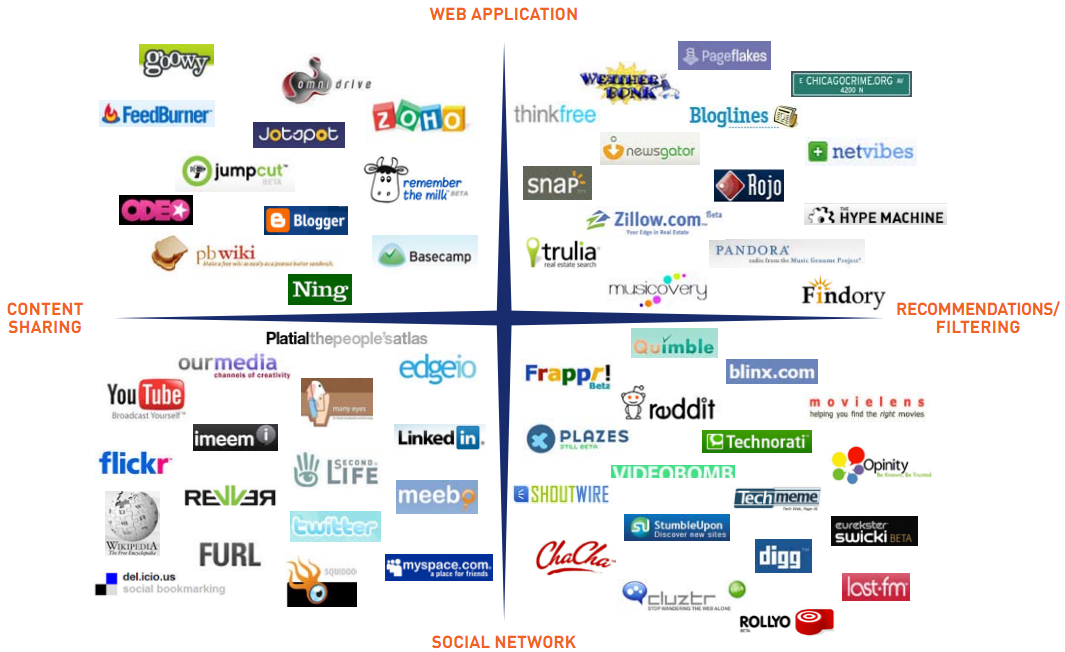
\includegraphics[width=1\textwidth]{CH4-F0-WEB20}
\caption[Web 2.0 Landscape]{Web 2.0 Landscape \citep{Dawson2007}}
%http://www.rossdawsonblog.com/Web2_Framework.pdf
\label{fig:web20l}
\end{figure}

Although there is no official classification of Web 2.0 resources, they can be
categorised as shown in Figure \ref{fig:web20l} by grouping these resources
according to their primary purpose. While this classification is not very
important for the context of this thesis, the figure illustrates the large
variety of Web 2.0 resources available online. Particularly this figure captures
only 62 Web 2.0 companies and applications considered to be prominent by
\citet{Dawson2007}. The actual number of such resources is much bigger. For
example, the largest Web 2.0 directory,
Go2Web20\footnote{\url{http://www.go2web20.net} (Accessed April 16, 2012)},
accounts for more then 3000 active resources and services, and this number grows every day showing the high
popularity of Web 2.0.

Based on statistics and publications on the Internet (as can be found by
searching for the keywords \textit{Internet statistics}, \textit{Web 2.0 statistics}, and \textit{Web 2.0
resources popularity}\footnote{As of February 2012}), the most popular Web 2.0
tools, services and resources are the ones that allow:

\begin{itemize}
  \item Create and publish information (e.g. blogs) 
  \item Collaborate with others (e.g. wikis)
  \item Network and build community (e.g. forums, social networking sites)
  \item Share personal stories with the world (e.g. podcasts)
\end{itemize}

These Web 2.0 tools promote a \textit{culture of participation}
\citep{Shelly2011} which might explain their attractiveness to the users. For
example, wikis encourage users to collaborate on creating, organizing, and
publishing information while discussing content and sharing knowledge. Whereas
wikis have become a popular tool for collaboration, blogs have been primarily
used by the individuals for various purposes. Blogs give the users an
opportunity for self-expression and sharing experience as well as promoting
their businesses or professional expertise. Another widely used way of sharing
personal stories with the world is podcasts. Such popular resources as YouTube
and iTunes allow users to upload and broadcast media files, both audio and
video. Social networking sites (e.g. Facebook, Google+, LinkedIn, MySpace) are
aimed to connect people who have common interests and goals. They give a high
level of interaction between users, a sense of community, and shared emotional
connection \citep{Zhan2010}. A notion of public opinion is present through the
commenting feature which the majority of the above mentioned Web 2.0 tools have.
In comments users can give feedback, discuss ideas, and share their view of the
topics of interest.

Web 2.0 plays an important role in today's society and is used for social and
commercial purposes. Examples from a variety of areas show the popularity and
impact of Web 2.0: virtual sports leagues attract millions of participants
\citep{Holahan2006}; politicians use blogs and podcasts in fighting for votes
\citep{Capell2006}; business models are changing, trying to adopt Web 2.0
characteristics \citep{Wirtz2010}; communication with customers is used to
increase revenue \citep{Havenstein2007}; communication pathways in research
communities are changing \citep{Ashling2007}; Web 2.0 portals are used in health
care to increase access to and enrich the quality of the information available
\citep{Gorlitz2010,Metzger2011}; video-blogging facilitates new ways of sharing
\citep{LibraryTechnologyReports2007}; the music industry is being transformed
\citep{Holahan2007}; genealogy research has become accessible to the public
\citep{MacMillan2007}; the tourism industry is adopting Web 2.0 technologies to
enhance customers' travel information and simplify access to the booking engines
\citep{Leung2011}.

Certainly, not all uses of Web 2.0 are linked to learning, especially when
thinking of the university context. But, in light of the \LLLs skills expected
from today's higher education graduates, the potential of Web 2.0 for supporting
learning becomes obvious \citep{Tian2011}. This potential is confirmed by
research studies that investigate the links between the two areas: Churchill
\citeyearpar{Churchill2009} examines the use of blogs in support of learning;
Wheeler, Yeomans and Wheeler \citeyearpar{Wheeler2008} look at student-generated
content using wikis; Boulos and Wheeler \citeyearpar{Boulos2007} investigate Web
2.0 tools for social communication in a learning context; Klamma and his team
\citeyearpar{Klamma2007} analyse a potential use of social software for
collaboration and informal learning. Yet, when designing education that
integrates Web 2.0 technologies the skill levels of students have to be
considered. While it is widely assumed that today's student generation is
Internet savvy, it has to be acknowledged that quite a number of students have
limited Web 2.0 skills. They are either not familiar with the technologies, or
have only basic level skills \citep{Kennedy2008,Hosein2010,Jones2010}.

\section{Gap Between Learning Environments}
Students in universities have access to both environments, the institutionally
controlled LMS and the participatory managed Web 2.0 resources and services. On
the whole, these two virtual worlds remain separate, both in the students' and
the institutions' minds, with a distinction being made between \textit{serious
learning} and \textit{play} \citep{Freire2008}. Many students cannot transfer
their technology skills employed in a social Web 2.0 context into academic
learning, which is both a motivational and a skill transfer issue
\citep{Katz2005}. The information technology sections of universities draw a
clear line between institutionally provided, controlled and supported LMS
services and the \textit{wild west} of the Web \citep{Havenstein2007a}. While
they cannot effectively restrict access to Web 2.0 tools, they can deny
institutional support and responsibility for quality of service. Educational
researchers and individual academics have identified the potential of social
networking tools for teaching and learning. This has led to the incorporation of
open access Web 2.0 tools into some courses at universities, as has been
illustrated earlier in this chapter.

In response to the popularity of Web 2.0 tools and their potential for learning,
LMS system providers have started to integrate social networking functionality
into their systems (as can be found in functional specifications of system
vendors). Discussion forums, blogs and wikis have been added to the tool-sets of
LMS. Yet, the important Web 2.0 characteristic of open access has been removed
as these tools have been bound into the institutional LMS framework. Access is
linked to course enrolment and under institutional control. Student-generated
content is accessible to the lecturers in charge and tool use is directed by
relevance to the respective course. The value for teaching and learning remains,
but learning is limited to the boundaries of course content and purpose
\citep{Mott2010}.

Facebook and Blackboard LMS can serve as an example that the gap between
these environments is wide and not easily bridged. An integrated application
using the Facebook social networking platform was included into the Blackboard
Learn software. Blackboard Inc. believed that such an approach would enable
students to stay connected, not only inside their classroom, but also outside
\citep{BlackboardInc.2009}. However, reviewing users' feedback on the Web (as
can be found by searching for the keywords \textit{Blackboard},
\textit{Facebook} and \textit{integration}) shows that this integration approach
was not accepted by the learner community. Users were concerned about
application security and the privacy of information stored in this social
networking environment. A number of students hesitated conducting their social
communication in such close proximity to their classroom work. 

Considerations outlined in this section bring up a need for a virtual space that
has to meet the requirements for successful \LLLs (based on Chapter
\ref{cha:litrev} recommendations) and facilitate the development of \LLLs
skills. This space has to be integrated into university environment and
accepted by student learners. It has to bridge institutional and personal
learning. The virtual space has to be safe, secure and provide students with a
long-term access. It should also facilitate both formal and informal learning
and allow for social networking and for collaboration. Such a space needs to put
students in charge of their learning and offer them privacy for exploration,
while still allowing for guidance from the lecturers. It should allow students
to continue learning informally even upon completing the formal courses (and
losing access to the LMS artifacts). This space has to provide a long-term
accessible, safe repository for storing artifacts demonstrating achievements. It
needs to be a \textit{professional} space that remains uncluttered from purely
social communication.

Taking into account all these requirements, the next section introduces \ep~as a
part of a university's learning environment that has the potential to provide
support for \LLLsn.

\section{ePortfolio}
For a long time physical portfolios have been used by artists as presentation
tools to collect, organize and showcase their artwork. The aim was to convince
potential customers of the artists' competence. Starting from two decades ago,
portfolios were adopted by educators to assess the quality of teaching
\citep{VanTartwijkJ.2004}. Since then portfolios have been used for many
different purposes and as a consequence portfolio types such as showcase,
development and assessment have been defined.
 
Electronic portfolios or ePortfolios are a digital representation of physical
portfolios. The EDUCAUSE National Learning Infrastructure Initiative
(NLII)\footnote{\url{http://www.educause.edu} (Accessed April 16, 2012)} (cited
by \citealp{IMSGlobalLearningConsortium2005}) defines ePortfolio as:

\longquote{ePortfolio is a collection of authentic and diverse evidence, drawn
from a larger archive, that represents what a person or organization has learned
over time, on which the person or organization has reflected, designed for
presentation to one or more audiences for a particular rhetorical purpose.}

\subsection{Characteristics of Portfolios and ePortfolio Systems}
\label{sec:charep}
The term portfolio is used in many different ways. As was already mentioned, an
important distinction can be made along the lines of the portfolio's purposes,
namely for development, showcase, assessment or competences
\citep{VanTartwijkJ.2004}.

Development portfolios or repositories support the learning and development of a
learner over a period of time. They contain material and artifacts related to
learning, reflections and feedback. It is important that the material stored in
these repositories is private to the learner. It is up to the learner to decide
when and what to share with whom. The learner needs to reflect on the material
collected and on his/her development in relationship to criteria or skills. The
giving and receiving of feedback are important aspects of the learning processes
around development portfolios.

Showcase portfolios tend to display examples of a learner's best work. These
presentations contain reflection and supporting evidence. They are composed for
a specific purpose and audience, e.g. a review committee, potential employer or
sponsor \citep{Lorenzo2005}.

Portfolios are often linked to assessment. The type of portfolio and type of
assessment have to be carefully adjusted to each other. Assessment portfolios
demonstrate learner's competencies and skills in well-defined areas. They can be
used for both formative and summative assessment. For formative assessment the
learner documents work and reflects on it, the assessor provides feedback that
assists the learner in future development. Summative assessment requires
predefined criteria of what is to be assessed allowing the learner to organize
work examples according to these criteria. In the design of the assessment
approach one has to be very careful to specify clearly what is to be assessed:
subject specific work, reflections, \LLLs skills, or presentation.

Portfolios for competences combine elements of both development and showcase
portfolios and are, to a certain degree, linked to assessment. In professional
areas, like health services, teacher education or engineering, the accreditation
of graduates and the continuing accreditation of professionals are often linked
to the demonstration of competencies \citep{IPENZ2007,Sullivan2004,Boyatzis2008}.
Portfolios have proven to be excellent tools for this process. The candidate
collects evidence, reflects on their practice and might invite feedback, all
processes covered by portfolio approaches. The accreditation occurs based on the
information provided in the portfolio.

Despite these variations, there are several key processes included in most if
not all portfolio work \citep{Malloff2010, Heinrich2012}, as displayed in
Figure \ref{fig:ep}.

\begin{figure}[hb]
\centering
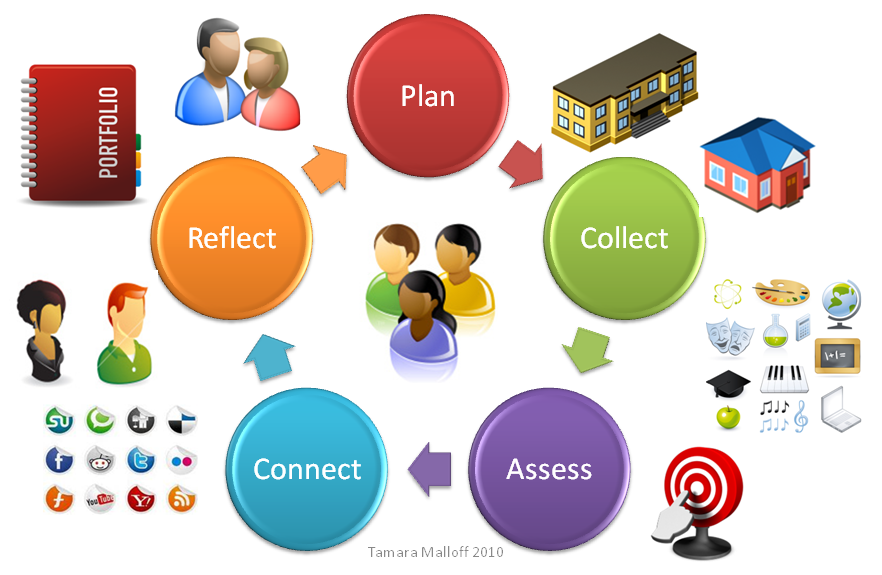
\includegraphics[height=0.47\textwidth]{CH4-F1-EP}
\caption{ePortfolio key processes}
%http://www.flickr.com/photos/kootenayleadership
\label{fig:ep}
\end{figure}

Similarly, Cambridge \citeyearpar{Cambridge2010} emphasized the importance of
the following activities in portfolio process:

\begin{itemize}
  \item Capture -- collecting/gathering information and evidence from various
  sources;
  \item Management -- aggregating captured evidence, sorting, indexing, ensuring
  accessibility over time;
  \item Reflection -- making sense of evidence, understanding own experience and
  achievements;
  \item Composition -- linking up the components together and making them
  available to others;
  \item Analysis -- understanding if additional evidence is needed, reflecting
  on feedback, keeping up dialogue with others.
\end{itemize}
 
While portfolio work can be conducted without the help of electronic systems,
such systems assist with many tasks around document collection, recording of
information, sorting through data and communicating with others. According to
Tosun and Baris's \citeyearpar{Tosun2011} research, \ep~compared to portfolio
has valuable extra features such as: a wider context and serving different
groups; archiving; cooperation and reorganization; publication and link building.
Many systems, from general Web tools to specialised applications, can be used to
support portfolio work. A comprehensive overview can be found at Helen Barrett's
ePortfolio web-site \citep{Barrett2008}. 

Using the specialized \ep~systems has its benefits over the non-specialized
approach. One of the benefits is that the specialized systems have clearly
defined centralized access control to the resources. For example, when a user
who is employing a wide range of different Web tools for \ep~work wants to share
their \ep~with others, they needs to make sure that all the artifacts in this
portfolio have the same access level and the reviewers will not come across the
``access denied'' items. In addition to centralized access control, the
specialized \ep~systems have a centralized repository which makes selecting,
aggregating and showcasing examples and artifacts easier and less time
consuming. For evaluation and feedback purposes, the specialized approach is
better for managing shared resources where the artifacts have potentially to be
locked so that changes cannot be made during the assessment time. From the
technical support perspective, the specialized systems are easier to maintain
and ensure that all users have the same high quality of services. For all these
reasons, this thesis is going to focus on systems specialised for portfolio
work.

\ep~systems are centred around the individual and their needs. They provide the
individual with a space for storing documents of any electronic format. In this
space the user creates a repository of artifacts related to all aspects of their
learning and professional development. There are tools for reflection, commonly
in form of blogs. In contrast to open Web 2.0 systems, access to both files and
reflections is by default set to the individual. Unlike in the LMS, there is no
hierarchy between users in which one higher-level user could see the work of a
lower-level user. The individual can select to share their work with others and
has full control over whom to share with and for which period of time. 

\ep~systems provide easy to use tools for constructing presentations that
combine artifacts and reflections and that can voluntarily be shared with others
or removed from public access at any time. The systems allow each individual to
form groups and identify partners for exchange. To a varying degree the
\ep~systems incorporate guidance towards reflection and self-directed learning.
\ep~systems provide a set of features that in combination are well suited to
support \LLLsn.

Each of the above mentioned features looked at separately can be found in other
computer systems or Web 2.0 tools. For example, blogs can be used for
reflection, computers' hard drives with all their disk and folder structure can
be suitable for a portfolio repository, email can serve as sharing and giving
feedback method, etc. However, the combination of these features within one
system is what makes \ep~systems so valuable.

\subsection[ePortfolio Systems Overview]{ePortfolio Systems
Overview\footnote{The \ep~systems in this section will appear in alphabetical
order.}} 
The following sections explore the features and functionality of various
\ep~systems. These specific systems were chosen for their level of success in
learning communities and current development status. Four proprietary
(PebblePad, BlackBoard \ep, Desire2Learn, eFolio) and two open-source (Mahara,
ELGG) systems are reviewed and analysed. Where possible, proprietary systems
were reviewed by accessing demonstration web sites. When demonstration web
sites were not available, the systems were reviewed by analysing user or
administrator documentation, video demonstrations, attending demonstration
seminars, and external reviews. If not specified otherwise, any material in
the systems overview can be referred back to the developer's official web site.

It is important to note here that this section is not aiming to find the best
system, but rather to evaluate \ep~systems that are currently available and
successful. Examining strengths and weaknesses of these systems can provide a
better foundation for understanding and development of an \ep~aided environment
that can provide comprehensive support for \LLLsn.

\subsubsection{BlackBoard ePortfolio}
In 2006, a popular LMS provider
BlackBoard\footnote{\url{http://www.blackboard.com} (Accessed April 16, 2012)}
developed an \ep~toolkit the most recent release of which is currently a part of BlackBoard Learn 9.1.
This \ep~system is designed as an add-on to the LMS environment and cannot be
used as a stand-alone product. On one hand, it means that all users must have
BlackBoard LMS account to be able to access \ep. On the other hand, it gives
some advantages which other \ep~systems might lack, such as single sign-on with
LMS, direct import of graded materials from Blackboard courses and links to
course goals and objectives.

BlackBoard \ep~is available in Basic and Personal Portfolio versions. Basic
Portfolio has an \ep~set-up wizard for learners who need guidance. However, it
is largely dependent on functionality available in the LMS. Without activation
of various features, the repository might be restricted to text and hyper-links
only. Personal Portfolio provides more flexibility and functionality. Therefore,
this version will be reviewed further as BlackBoard \ep~(Figure \ref{fig:bbep}).

\begin{figure}[htb]
\centering 
\setlength\fboxsep{0pt}
\setlength\fboxrule{0.5pt}
\fbox{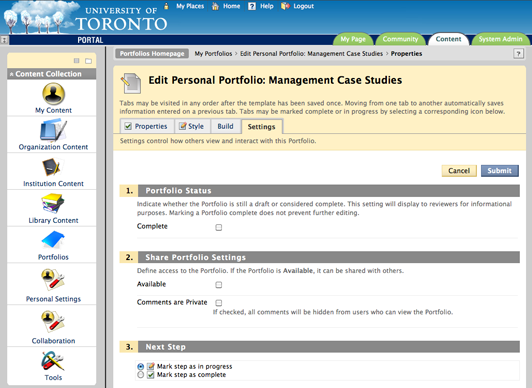
\includegraphics[width=0.9\textwidth]{CH4-F6-BB}}
\caption[BlackBoard ePortfolio example]{BlackBoard ePortfolio example
\citep{UniversityofTorontoScarborough2010}}
\label{fig:bbep}
\end{figure}

In the system, ePortfolio owners have control over the content, access, layout
and style of their portfolio. ePortfolios can be created from available
templates predefined by an administrator or a lecturer, or they can be created
from scratch. A variety of video, audio and text file types is supported as well
as an HTML editor for creating pages. Reflections are facilitated in the form of
blogs or threaded topics. Content is separated from portfolios which allows
reuse of the artifacts. It has been reported that because of this separation
artifact management is not intuitive and might be too complex for students for
effective use of the tools \citep{Clark2009}. In addition, portfolios can be
linked to learning objectives defined by lecturers, administrators or learners
themselves.

When necessary, BlackBoard \ep~can be shared with people inside the
institutional community through system username, groups and courses as well as
outside -- via email or creating a guest account which is by default active for
30 days. However, availability of these sharing options is set up by system
administrator who can allow or restrict any of these options. Depending on
access level, users can leave their feedback in the form of comments. Comments
cannot be attached to individual artifacts and are stored within single pages of
\ep. BlackBoard \ep~system has a basic reporting system where users can enable
tracking, and gather basic data about views of their portfolios. At the
completion of studies \ep~can be downloaded and saved as HTML in a ZIP archive.

Overall, BlackBoard \ep~is good for creating portfolio of student course or
program work and for linking to a course of study
\citep{UniversityofTorontoScarborough2010}. 

According to \citet{Sweat-Guy2007}, the cost of 12 months license for
BlackBoard \ep~in 2006-2007 was 20,900USD per institution which did not include
the cost of prior purchase and adoption of LMS. To date, no information was
found on current development status and future releases.

\subsubsection{Desire2Learn}
Desire2Learn\footnote{\url{http://www.desire2learn.com} (Accessed April 16,
2012)} \ep~is a proprietary \ep~system developed by Desire2Learn Incorporated. It can be deployed as a
standalone application or as a part of a Desire2Learn Learning Environment. As a
result of close working relationship of the developing company with Microsoft,
this \ep~system, as well as all Desire2Learn software, is built on Microsoft
technologies, such as SQL Server and Windows Server \citep{AAEEBL2011a}.

Most artifacts can be uploaded to the system from external resources. Some of
them, such as HTML files, can be created within the environment. This also
includes creating audio recordings which is a unique functionality compared to
other \ep~systems. Currently, Desire2Learn developers are looking into adding
support for creating of video records.

There is a standard range of functionalities associated with artifacts in this
ePortfolio system: they can be grouped, shared with others, commented on,
assessed directly or submitted as an assignment. Assessment results, such as
grades, competencies or quiz details, can be saved as \ep~artifacts as well.

\begin{figure}[htb]
\centering
\setlength\fboxsep{0pt}
\setlength\fboxrule{0.5pt}
\fbox{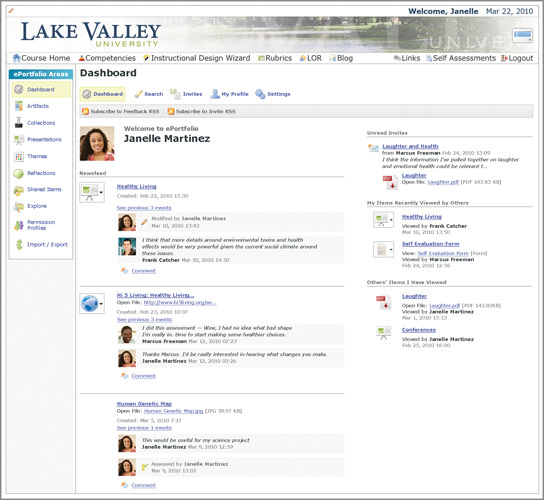
\includegraphics[width=0.9\textwidth]{CH4-F7-D2L}}
\caption[Desire2Learn ePortfolio example]{Desire2Learn ePortfolio example
\citep{Desire2LearnIncorporated2011}}
\label{fig:d2ep} 
\end{figure}

In addition to individual artifacts, other types of items in the \ep~system are
collections, presentations, reflections and forms. Collections are used to group
artifacts and can be created manually or automatically based on a defined tag
set. Forms provide a way of developing artifacts with standard field types. This
can be used for creating templates for evaluations, resumes, or self-evaluation.
Presentations are personal web sites that present a set of artifacts in an
organized way allowing users to choose theme, set up layout and manage content
(Figure \ref{fig:d2ep}). Reflections are a separate form of the artifacts. They
can be associated with artifacts or presentations and can be a part of
collection or presentation.

Feedback can be applied to individual artifacts, collections, reflections or
entire presentations. If needed, evaluators can review all comments made by
peers. Users can add assessment rubrics to artifacts that require specific
type of evaluation. More comprehensive assessment features are available via
integration with other Desire2Learn LMS tools. 

Desire2Learn \ep~has reporting capabilities for administrators and teachers
which support tracking usage and accessing detailed information on competency
achievement by students. Minor reporting is available to users in form of
presentations access logs.

Any part or an entire \ep~contents can be imported or exported using either XML,
or HTML format. XML is a native format of the system and allows the import of
\ep~to another Desire2Learn \ep~system instance.

No estimate cost of the Desire2Learn \ep~was discovered as vendors do not
disclose pricing information, explaining that each case is unique to each
institution.
 
\subsubsection{eFolio}

The eFolio\footnote{\url{http://www.avenetefolio.com} (Accessed April 16, 2012)}
system is a software service hosted and maintained by Avenet Web Solutions. Developed in 2001
together with the University of Minnesota, eFolio currently has a large user
base, the biggest of which are
eFolioMinnesota\footnote{\url{http://www.efoliominnesota.com} (Accessed April
16, 2012)} (over 60,000 active users) and
eFolioWorld\footnote{\url{http://www.efolioworld.com} (Accessed April 16, 2012)} (over 34,000 active users) \citep{AAEEBL2011}. Although eFolio is a hosted service, it
is still possible to get self-hosted solutions for very large implementations.

Every account in eFolio can have multiple portfolios which are organized as
sites. When users start creating a site, they can use a wizard under the ``To
Do" category for filling the pages with the relevant content. The latest version
of the system has a drag and drop site management interface which makes it easy to
create sites and pages. eFolio comes with a number of build-in display and style
formats. However, according to the comments \citep{AAEEBL2011}, the system
does not provide as much page layout flexibility as some users would expect.

Everything saved in eFolio is located in the ``My Content'' category. Currently,
its standard storage capacity is 50MB per user, but this limit can be
negotiated. My Content groups items by data types such as artifacts, courses
taken, goals, images, URLs, employment, etc. As well, users can add or create
the items on the fly while building their sites. Users can set up content
properties and formatting, add other content related to the item and write
multiple reflections.

All sites are by default private, but can be set to public once finished.
Under-age user sites are always private by default and cannot be made public.
Alternatively, owners can invite a specific person to review their site. Access
to the web site is granted through creating visitors. Each visitor gets an email
with login details if the site is private or site URL if it is public. Even
users who already have accounts in the system get a visitor account for each
specific site access. Visitors can leave feedback to any item with feedback
properties set up. Depending on these properties, feedback can be in the form of
Likert scale, question/answer or free-form text.

\begin{figure}[htb]
\centering
\setlength\fboxsep{0pt}
\setlength\fboxrule{0.5pt}
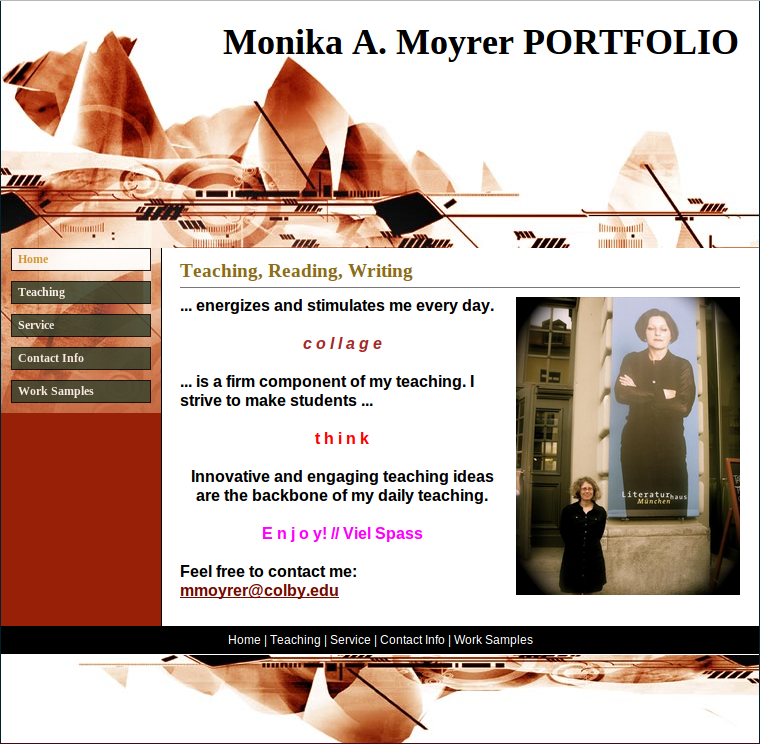
\includegraphics[width=0.87\textwidth]{CH4-F8-eFolio}
\caption[eFolio system example]{eFolio system example \citep{EFolioMinnesota2011}}
\label{fig:efolio}
\end{figure}

eFolio does not provide collaboration functionality and all web sites in the
system are personal (Figure \ref{fig:efolio}). For assessment purposes eFolio
has questionnaires of various types which students can use to address assessment
criteria.

eFolio supports the IMS ePortfolio standard \citep{AAEEBL2011} which allows
users to import/export their ePortfolio content. The system can be integrated
with the Moodle LMS. However, no detailed information was found on what kind of
integration this is.

After graduating or leaving a sponsoring institution, users can continue
using their eFolio for an annual fee of 15USD. Prices for institutions depend
on numbers of users, and can range between 15USD - 4USD per user
\citep{AAEEBL2011}.

\subsubsection{ELGG}
ELGG\footnote{\url{http://elgg.org} (Accessed April 16, 2012)} is an open source
social networking and social publishing platform started in 2004 and released under the GNU
General Public License
v2\footnote{\url{http://www.gnu.org/licenses/gpl-2.0.html} (Accessed April 16,
2012)}. It was originally aimed at higher education, but is currently used in many contexts from business
to sport. Developers of ELGG call it a \textit{social engine to empower social
environment}.

Features available in the standard platform installation include user management
and administration, social networking components (like friends list and ``the
wire''), blogging, message board, file repository, private messaging, pages, and
bookmarks. Additional components can be installed by administrator as plugins
and can be used within the entire system.

Most the end-user functionality comes from plugins which can be loaded into the
system. This review examines a standard installation. ELGG is supported by an
extensive community which has contributed a large number of plugins. In general,
most of these plugins are aimed at supporting social networking.

Unlike other ePortfolio systems, ELGG has a quite limited choice of permissions.
Artifacts in the system can be either private/public, or shared with friends
or logged-in users. There is no way of having multiple permission settings or
user-to-user permissions for artifacts.

In ELGG, each account has a profile page (Figure \ref{fig:elgg}) which links to
all available artifacts created by the user through adding or removing widgets.
Except for the profile page, there is no standard way of aggregating artifacts
for presentation. The profile page is as well the main option for showcasing as
users cannot have multiple ePortfolios.

\begin{figure}[htb]
\centering
\setlength\fboxsep{0pt}
\setlength\fboxrule{0.5pt}
\fbox{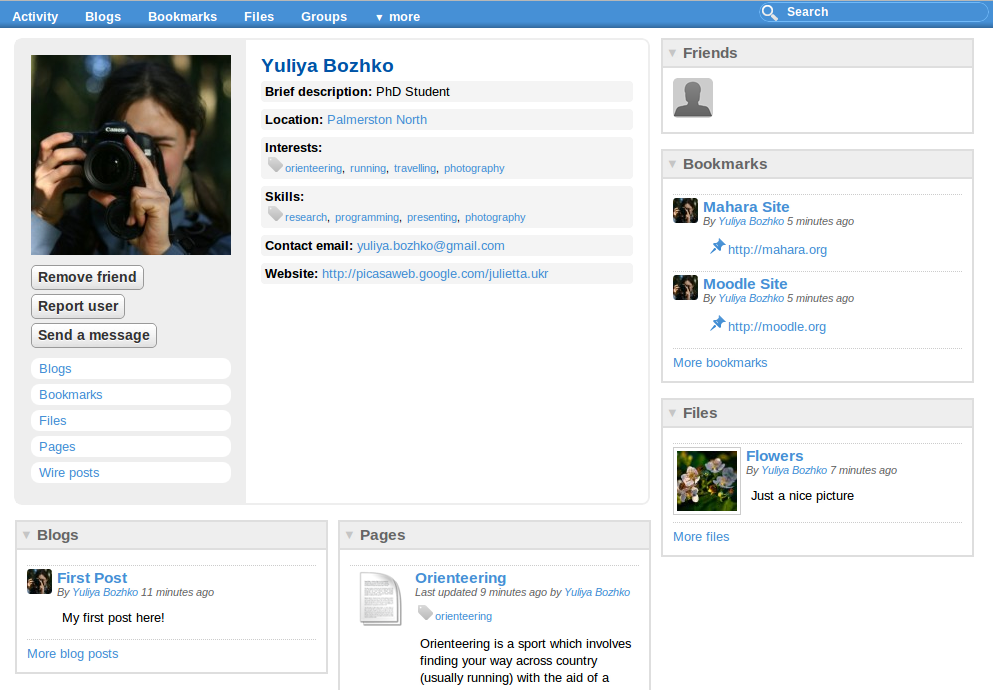
\includegraphics[width=0.9\textwidth]{CH4-F5-ELGG}}
\caption{ELGG 1.8 example}
\label{fig:elgg}
\end{figure}

Similarly to some other \ep~systems, ELGG has groups for collaboration. Groups
have the same system components (e.g. blogs, pages, files) as single profiles,
and these options can be set up or removed at any time.

ELGG has no reporting system for users which would show a number of page
visits, file downloads, etc. However, minor reporting functionality is available
for administrative purposes.

In 2007, interoperability between ELGG and the open source LMS Moodle was
established for single sign-on and courses integration. However, since Moodle
1.9 there is no news on plugin updates. Information has been found on the
Internet about a proprietary plugin being developed for ELGG-Moodle integration,
although no up-to-date documentation is currently available that would describe
this plugin.
 
\subsubsection{Mahara}
Mahara\footnote{\url{http://mahara.org} (Accessed April 16, 2012)} is an open
source \ep~system started by a group of education academics at Massey University in 2006 funded by the New
Zealand Tertiary Education Commission \citep{Brown2007}. The system is a
standalone application and does not require any kind of LMS or other system
installed. Its modular and extensible architecture resembles the architecture of
Moodle LMS. This can be explained by the fact that developer community of Mahara
is deeply involved in the Moodle community. The system is claimed to be highly
\textit{pluggable} which allows adding various Web 2.0 web services and
establish interoperability with other systems \citep{MaharaGovernanceGroup2011}.

Mahara functionality includes a number of standard \ep~features like file
repository, reflection tools in form of blogs, presentation and sharing tools as
well as elements of social networking like friends lists, forums, message board
and e-mail. Mahara has an internal r\'{e}sum\'{e} builder which allows users to
create their digital CV with various information options. Sharing is done
through pages which are called \textit{views} (Figure \ref{fig:maharaep}). Users can
create single views or collections of views and fill them with artifacts from
their \ep~repository. Views can be created from scratch as well as from a
template developed by another user.

\begin{figure}[htb]
\centering
\setlength\fboxsep{0pt}
\setlength\fboxrule{0.5pt}
\fbox{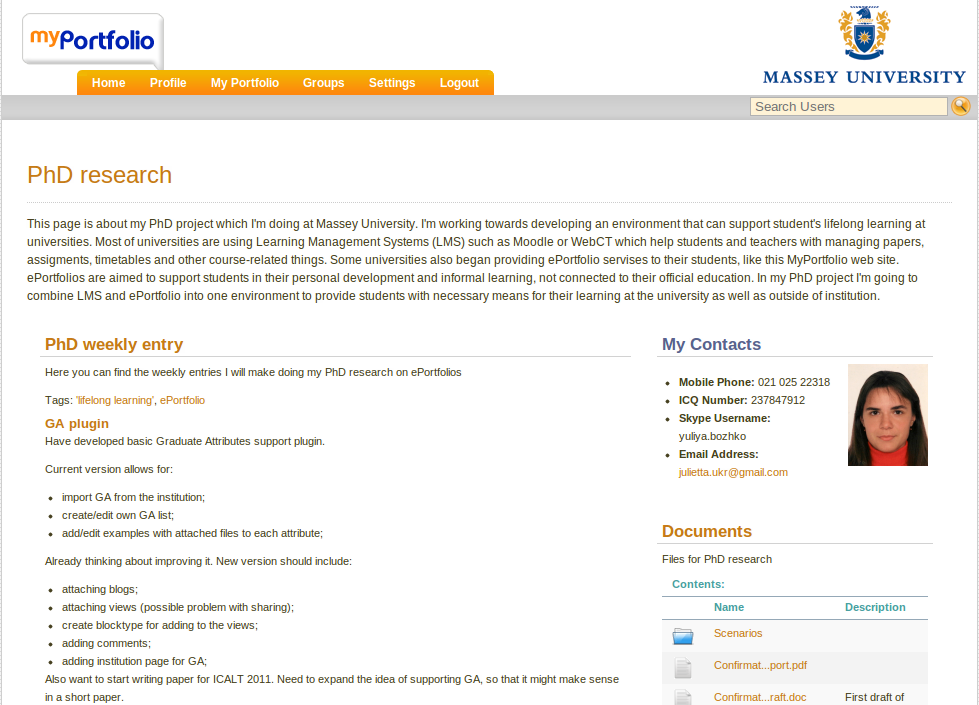
\includegraphics[width=0.95\textwidth]{CH4-F4-Mahara}}
\caption{Mahara ePortfolio 1.3 example}
\label{fig:maharaep}
\end{figure}

A group portfolio is available for collaboration purposes. Compared to personal
accounts, groups have functionality limited to creating and maintaining pages
(views), forums and file repository.

As it became popular in \ep~systems throughout the recent years
\citep{Waters2009}, Mahara comes with a user-to-user permissions control. Users
can set up three levels of access to parts of their \ep s (private, individual
and public) which defines what items and information others can see. Currently
the Mahara system does allow sharing views with others or making them public,
but giving feedback is restricted to registered users.

Mahara supports a complete LEAP2A interoperability
\citep{MaharaGovernanceGroup2011} which allows the import of portfolio content
to Mahara and export to another \ep~system, provided that this interoperability
standard is implemented on the other side. In addition, export in form of static
HTML pages is supported.

The latest version of Mahara supports single sign-on with Moodle, which means
that users can log on to both systems using only one account. Unofficial plugins
developed by the community allow for submitting views as assignments to Moodle.
However, this functionality is not included in official release. The road-map of
Moodle 2.0 included a repository plugin for Mahara that would allow direct
export of artifacts from LMS to \ep. Meanwhile, Moodle 2.1.1 release still does
not support this functionality.

\subsubsection{PebblePad}

PebblePad\footnote{\url{http://www.pebblepad.co.uk}} is a proprietary web-based
\ep~system. However, its designers tend to call it not just an \ep~system, but
Personal Learning System that can be used in a variety of learning contexts
\citep{PebbleLearningLtd2010}. The system is popular and primarily used in the
UK Higher Education sector and has been involved in a number of JISC funded
ePortfolio research projects including such projects as 
ePistle\footnote{\url{http://jisc.ac.uk/whatwedo/programmes/edistributed/epistle}
(Accessed April 16, 2012)} and
File-Pass\footnote{\url{http://jisc.ac.uk/whatwedo/programmes/edistributed/filepass} (Accessed April 16, 2012)}.

According to the PebblePad technical specification, the back-end of the system
requires Windows and SQL Servers to run. The front-end uses Flash, which can
create a challenge for the web application's accessibility, usability and
performance. To function, Flash-based applications require a plugin which in
turn might cause many standard browser features not to perform as the user would
expect or may even cause a browser crash. Flash applications do not work on many
mobile and portable devices. In addition, because Flash applications are
compiled into binary files, screen readers used on web sites that support the
sight impaired cannot read them which results in poor accessibility.

PebblePad has a customizable user interface (Figure \ref{fig:ppep}) which
includes user-defined size and style of text and background colours.
Institutions can have their own interface that fits in with the institutional
branding.

\begin{figure}[htb]
\centering
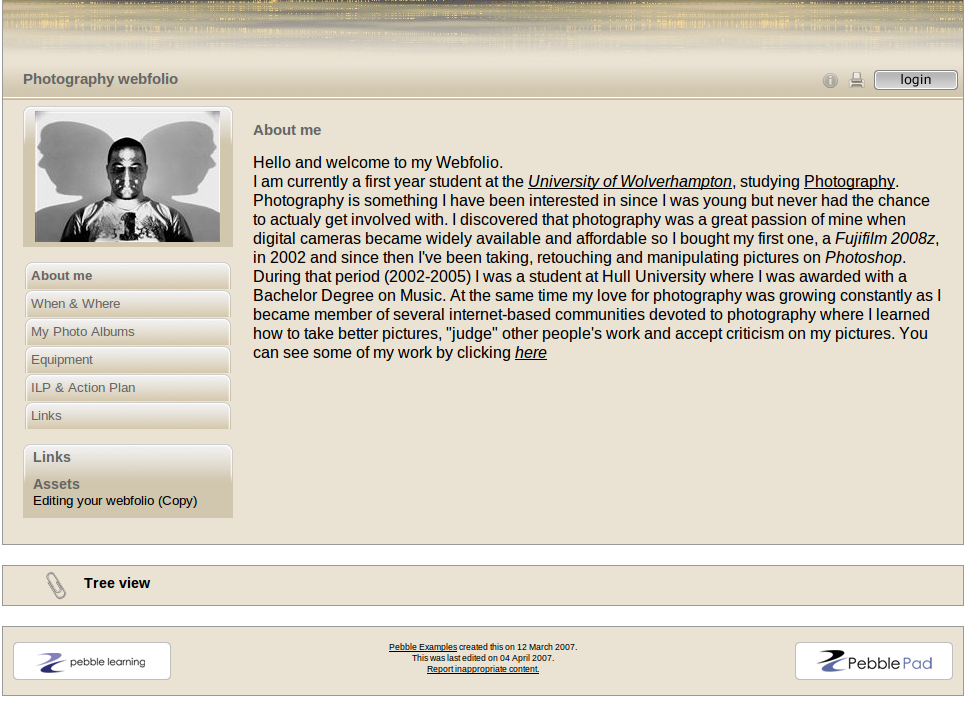
\includegraphics[width=0.9\textwidth]{CH4-F3-PebblePad}
\caption[PebblePad \ep~system example]{PebblePad \ep~system example
\citep{PebbleLearningLtd}}
\label{fig:ppep}
\end{figure}

Items stored in the PebblePad repository are called assets. There are thirteen
asset types that are subdivided into three core types, namely: uploaded files,
single assets and aggregating assets. Creation of some assets can be guided by
step-by-step wizard. Assets can be shared with others, inside or outside of an
institution, for a certain period of time through user-defined permissions. If a
person, who needs to see an asset, is not a part of the PebblePad community, a
temporary username and password will be automatically created allowing them to
view a shared asset. Assets allow for setting up a wide range of permissions,
which can include commenting and copying rights, collaboration and re-sharing
of a shared asset with a third party.

However, despite these features, working with assets in PebblePad has its
disadvantages. The way the system's repository is structured, asset tracking and
finding in PebblePad is noted to be not user-friendly \citep{Overton2009}. Due
to poor asset management, users can end up deleting files and breaking links
between assets, or forgetting to update the hyperlinks of the changed assets,
which results in missing files for someone who is viewing the asset. Users
cannot upload files larger than 10MB.

PebblePad has an interface with the Moodle LMS that allows \ep~users to have
single sign-on with LMS and also export items from Moodle to their ePortfolio.
The system supports Leap2a and IMS eP as well as import from any RSS or Atom
compliant system. According to the vendor's website, as at the middle of 2011,
the price of PebblePad adoption ranged from 14,95GBP per year for individual
accounts hosted by the company to 1GBP per user per year for the largest
customers hosting the system themselves. After graduation from the sponsoring
institution, students can get a free 12-month personal account managed by Pebble
Learning.

\subsubsection{Discussion}
The overview of the \ep~systems showed that they have relatively standard set of
features. All systems provide support for the key \ep~processes of collecting,
selecting, reflecting, planning and connecting as described in Section
\ref{sec:charep}. Collecting is usually done through gathering various files and
creating records in the systems. After information capturing is finished, user
can sort artifacts selecting the ones that can be used for intended purpose.
Reflection in the majority of the \ep~systems is supported through personal
blogs. Some systems (eFolio, PebblePad) also provide reflection options linked
directly to the individual artifacts. Planning is implemented in the form of
personal learning objectives or learning plans, although not all \ep~systems
have this feature. Connecting of artifacts is largely achieved through web pages
or other internal aggregation methods. All reviewed \ep~systems allow meaningful
collections of artifacts to be shared for feedback and assessment purposes.

Apart from common functionality, some of the \ep~systems have unique features
not present in the majority of other systems. Among these are:
\begin{itemize}
  \item Creating audio recordings within the \ep~environment (Desire2Learn)
  \item Individual items can have multiple reflections (eFolio)
  \item Social networking features (e.g., friends lists, message board, etc.)
  (ELGG, Mahara)
  \item Threaded topics for reflection (BlackBoard \ep)
  \item Initial set-up wizard (BlackBoard \ep, eFolio)
  \item Pluggable interface (ELGG, Mahara)
  \item Sharing of individual artifacts (eFolio, PebblePad)
\end{itemize}

\begin{sidewaystable} \scriptsize
\centering
	\caption{Mapping \ep~systems' features against \LLLs guidelines}
	\begin{tabular}{|c|p{3.25cm}|p{3.25cm}|p{3.25cm}|p{3.25cm}|p{3.25cm}|p{3.25cm}|}
	\hline
	 \multicolumn{1}{|c|}{} &
     \multicolumn{1}{c|}{\textbf{BlackBoard ePortfolio}} & 
     \multicolumn{1}{c|}{\textbf{Desire2Learn}} & 
     \multicolumn{1}{c|}{\textbf{eFolio}} & 
     \multicolumn{1}{c|}{\textbf{ELGG}} & 
     \multicolumn{1}{c|}{\textbf{Mahara}} & 
     \multicolumn{1}{c|}{\textbf{PebblePad}} \\ \hline
	\textbf{G1} & 
	Combination of \ep~and LMS supports all types of learning & 
	Combination of \ep~and LMS supports all types of learning & 
	Potential integration with Moodle LMS can cover support for all types of
	learning \textit{(No reliable information found)} & Potential single sign-on
	with Moodle LMS can cover support for all types of learning \textit{(No
	reliable information found)} & Integration with Moodle LMS covers support for
	all types of learning & Integration with Moodle LMS covers support for all
	types of learning \\ \hline \textbf{G2} & 
	-- Initial guidance through \ep~set-up wizard; \newline -- Guidance through
	 course goals and objectives; \newline -- Feedback in form of comments on
	web pages & -- Feedback on various types of artifacts; \newline -- Guidance
	through predefine competences in LMS; \newline -- Templates can be used as
	guidance & -- Feedback on various types of artifacts; \newline -- ``Getting
	started" Wizard for initial set-up & 
	Feedback on web pages and individual artifacts & 
	Feedback on web pages and artifacts on web pages; \newline -- Templates of web
	pages can be used as guidance & 
	Feedback on assets can be provided as guidance for students \\ \hline 
	\textbf{G3} & 
	-- Lecturers can define learning objectives; \newline -- Lecturers can provide
	feedback on shared resources & 
	-- Lecturers can define competences in LMS; \newline -- Lecturers can
	provide feedback and evaluate; \newline -- Lecturers can create templates for
	evaluations & 
	-- Lecturers can provide feedback on shared resources; \newline -- Lecturers
	can create templates to map competencies & 
	-- Lecturers can set up questionnaires; \newline -- Lecturers can provide
	feedback & 
	-- Lecturers can provide feedback on shared resources; \newline -- Lecturer
	can create templates of web pages & 
	Lecturers can provide feedback on shared assets	\\	\hline 
	\textbf{G4} & \textit{No information found} & \textit{No information found} &
	\textit{No information found} & \textit{No information found} & 
	\textit{No information found} & \textit{No information found} \\ \hline 
	\textbf{G5} & 
	\textit{No information found on collaboration} \newline -- Communication is
	in form of comments or through message center & 
	-- Collaboration through sharing; \newline -- Enhanced communication through
	LMS features & 
	\textit {No support for collaborative activities} \newline Integrated
	communication tools & 
	-- Groups are used for collaboration; \newline --	Communication is in 
	the form of comments, message board and internal message system & 
	-- Groups are used for collaboration; \newline -- Communication is
	in the form of comments, wall messages and internal message system & 
	-- Collaborative work with assets; \newline -- Communication is
	in the form of comments; \newline -- Assets re-sharing \\
	\hline 
	\textbf{G6} & 
	Data and grades export from LMS to \ep & 
	Data and grades export from LMS to \ep & 
	\textit{No information found} & 
	\textit{No data integration with external sources or LMS} & 
	Data export from LMS to \ep & 
	Data export from LMS to \ep \\ \hline
	\textbf{G7} & 
	-- Users can define learning objectives; \newline -- Users can
	associate artifacts with learning objectives & 
	-- Achievements can be recorded in form of presentations; \newline -- Users can
	set up personalized learning plans & 
	Mapping of specific competencies and learning outcomes into individual
	portfolios & 
	No specialized way or recording achievements. Blogs and pages can be used for
	this purpose & 
	-- Achievements are described as a part of user profile; \newline -- Users can
	create goals in form of plans & 
	Achievements can be recorded through the assets ``achievements''
	and ``experiences''	\\ \hline 
	\textbf{G8} & 
	Addressing high-order skills through defined by lecturers learning
	objectives / course goals & 
	Addressing high-order skills through assessment rubrics or integration with LMS
	& 
	Addressing high-order skills is done in form of web pages or tied to
	institutional rubrics & 
	Addressing high-order skills is done in form of web pages & 
	Addressing high-order skills is done in form of web pages & 
	Addressing high-order skills can be done in form of web pages or assets \\
	\hline 
	\textbf{G9} & 
	Reflections are in form of blogs and threaded topics & 
	-- Forms can be used for self-evaluation; \newline -- Reflections are a
	separate form of artifacts & 
	Individual items can have multiple reflections & 
	Reflection in the form of blogs & 
	Reflection in the form of blogs & 
	-- Reflection through wizard when creating assets; \newline -- Reflection in
	the form of blogs \\ \hline
	\end{tabular}
\label{tab:ep2map} 
\end{sidewaystable} 

Reviewing the \ep~systems from the \LLLs perspective requires looking further
than the key \ep~processes and activities. Suitability and ability of the
systems to provide support for \LLLs should be evaluated against the guidelines
and recommendations discovered in the literature (Section \ref{sec:needs}). Table
\ref{tab:ep2map} shows possible mapping of these recommendations to the features
of the reviewed \ep~systems. 

Exploration of these features from the \LLLs perspective showed that not all
guidelines are followed or supported by the \ep~systems. Particularly, no
information was found on the \ep~systems helping students to understand how they
learn and develop their skills through better organized learning materials.
However, while rigorous analysis has been attempted, a number of reasons have
hindered this analysis and suggest caution when looking at the findings.
Firstly, in some cases no reliable information was found to make unambiguous
conclusion. Secondly, the majority of proprietary systems were reviewed relying
on the sources of information other than first-hand experience of the researcher
which might have influence their trustworthiness. Finally, the guidelines
provided in the literature were not formal requirements and therefore their
assessment was largely done using analogical reasoning. Due to these issues, a
further exploration of the \ep~systems from the \LLLs perspective is required,
and the next section provides additional reasons for this.

\subsection{\ep~Systems in Light of Lifelong Learning}

Considering that the expectation around \ep~systems is that these systems
support \LLLsn, the question is whether they are doing it effectively in light
of the recommendations identified in the literature. Due to the fact that the
literature provides only highly conceptual recommendations, it is difficult to
translate these into formal requirements. Therefore, assessment whether these
recommendations are met by the features implemented in the systems turns into a
challenging task. 

The previous section described an attempt to address this problem trying to map
the recommendations against the features of the reviewed \ep~systems. However,
due to the highly conceptual level of these recommendations, the results of this
analysis should not be considered complete and final. As was explained earlier,
common sense and personal experience had to be followed to perform this
analytical mapping. To solve this problem, bringing the recommendations to the
practical level is the next important step towards a better understanding of
what is expected from the environment that can support \LLLsn. One can argue
that the majority of these recommendations cannot be addressed by just providing
an improved system \citep{Schaffert2008}. However, from another perspective, a
better system might aid to supporting various important aspects of learning that
usually stay outside of focus of many learning environments.

Although no prior research was found that would look at the \ep~systems from the
\LLLs perspective, there are a number of issues known among the \ep~community
that might be relevant to \LLLs support. For example, current \ep~systems have
difficulty helping students to link abstract knowledge to practical experience
which is an important part of understanding one's personal progress and
achievements \citep{Chou2009}. Interoperability between different \ep~systems as
well as other learning systems is quite poor despite the existing standards
\citep{Clark2011}. Assuming that \ep s are lifelong, they are supposed to cope
with large amounts of data \citep{Butler2010}. However, practice shows that
current systems can barely offer efficient methods for managing data
repositories to users who have been using them extensively for just a couple of
years. There are also issues of ethics, privacy and intellectual property where
\ep~users need to decide who owns the data and how it can be used
\citep{Challis2005}.

The problems mentioned here are just some examples that are not likely to draw a
complete picture. To get a deeper insight into \ep~issues and understand what
improvements are required for \ep~systems to fulfil the promise of efficient
\LLLs support, a deeper analysis of the area is required.

\section{Summary}

Based on the deliberations outlined in this chapter, additional conceptual
requirements can be considered along with the recommendations for successful
\LLLs support, such as:

\begin{itemize}
	\item A good virtual learning environment should facilitate the development of
	\LLLs skills;
	\item It should fit the university needs;
	\item It should fit the learners' needs and be accepted by students. 
	\item It should create a bridge between institutional and personal learning.
\end{itemize}

\ep~system seems to fit well into this picture. It brings a balance into the
world of learning environments, and has potential of closing the gap that exists
between LMS and Web 2.0. As was discussed earlier, LMS cannot provide the
required level of support for \LLLs as it is focused primarily at supporting
formal education. While Web 2.0 tools have the potential to do so, providing
quality of service for these tools in institutional settings is not feasible.

Reviewing \ep~systems showed that the systems currently available world-wide
offer a range of opportunities for \LLLsn. Each system comes with commonly
valuable functionality that promises support for important aspects of learning.
However, are they mature enough to be a part of the environment that provides
comprehensive support for \LLLsn? The previous section discussed that current
\ep~systems might still lack some elements important for \LLLsn. To support this
hypothesis, the next chapter will explore the needs for \LLLs supported by
\ep~systems based on the major stakeholders perspective. University students and
lecturers have been interviewed to get their insight on the requirements and to
understand whether these comply with the literature review findings.

\chapter{Stakeholders Requirements for \LLLc Support in Universities
\label{cha:model}}

\section{Lecturers' Perspective on \LLLc Support}
\subsection{Participants Profile}
\subsection{Methodology}
\subsection{Results}

\section{Students' Perspective on \LLLc Support}
\subsection{Participants Profile}
\subsection{Methodology}
\subsection{Results}

\section{Requirements Elicitation}

\section{Summary} 
\chapter{Prototype -- Development and Implementation\label{cha:prototype}}
%5020
This chapter presents design and implementation decisions for the \ep~aided
environment that provides support for \LLLs in universities. By the term
\textit{environment} this chapter describes a generic set-up of two
interconnected systems such as an \ep~system and LMS. For the development and
evaluation purposes, in this research, Mahara \ep~system was used as an
\ep~system and Moodle\footnote{\url{http://moodle.org}} was used as a LMS.

Previous chapters (Chapters \ref{cha:litrev} and \ref{cha:systudy}) identified
recommendations and needs for successful \LLLs support. With the help of the
major stakeholders, Chapter \ref{cha:model} took these highly conceptual
requirements to the practical level of the system features. Now, in this
chapter, development of these features using open-source \ep~system Mahara as a
basic platform for implementation is described.

This chapter starts with briefly discussing the overall architecture of the
environment and development toolkit. Then, each implemented component is
presented with its relation to the requested features and \LLLs recommendations
from the literature.

\section{Architecture}

Figure \ref{fig:arch} shows the overall architecture of the environment which
consists of two main components: institutionally controlled LMS and an external,
but institutionally supported \ep~system. The systems are connected in terms of
data exchange and users account management. LMS provides resources for formal
learning along with its outcomes which can be transferred to \ep~system. Being
hosted outside of institutional barrier, an \ep~system provides students with
private space for personal development and informal learning.

\begin{figure}[htp]
\centering
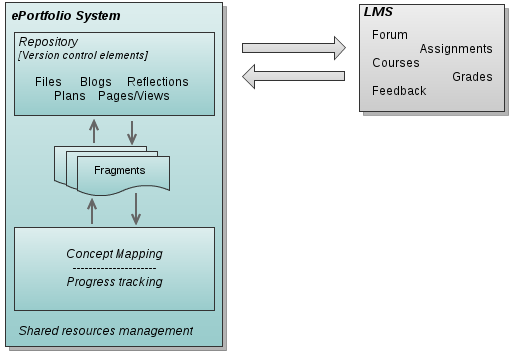
\includegraphics[width=0.9\textwidth]{CH6-F1-Architecture}
\caption{Environment architecture}
\label{fig:arch}
\end{figure}

In this project, the main implementations were carried out in the \ep~system
environment, Mahara. Due to cost vs benefit issues, features that involved LMS
environment, Moodle, were not considered for development. 

Benefit was analysed based on how high the interview participants had ranked
their requirements for \LLLs support. According to this, LMS aspects of system
support had not been identified as highly important in \LLLs context. 

The cost was measured by referring to the LMS developing communities that had
\ep~and LMS integration on their road-maps. For example, based on the issue
MDL-14591\footnote{\url{http://tracker.moodle.org/browse/MDL-14591} (Accessed
April 16, 2012)} on the Moodle LMS issue tracking system, it took one developer
from the development team, who probably had already been familiar with the
environment and its APIs, more than two years to develop an \ep~API that would
support single sign-on and enable simple data export/import functionality. To
date, this functionality still has a large number of unresolved issues and bugs
that require fixing (as can be seen from searching ``portfolio'' in Moodle Issue
Navigator\footnote{\url{http://tracker.moodle.org/secure/IssueNavigator.jspa}
(Accessed April 16, 2012)}).

As another example, based on discussions from ``Moodle and Elgg in Education''
group\footnote{\url{http://community.elgg.org/pg/groups/1057}
(Accessed April 16, 2012)} of Elgg community, more than 100 days were spent on development of a proprietary
plugin that would allow single sign-on and getting user statistics from Moodle
to Elgg.

Therefore, it can be concluded that investment into time and resources for the
development of the features that would allow integration between the systems
would exceed the benefit that would be gained from them by the users.

For these reasons, guidelines (G1 and G6) and features, that would have involved
modifications of Moodle LMS, were not realized by implementations and are not to
be discussed further in this chapter. However, for completeness, LMS is still
included in overall architecture as a system that supports formal learning in
universities.
 
Features identified through the interviews with the stakeholders were grouped
(based on groups described in Table \ref{tab:req}) and developed in the
following components and modules:

\begin{itemize}
  \item Version control -- for addressing the issues of guidance, facilitation
  and communication for \LLLsn;
  \item Artifacts' fragments extraction -- for better communication of specific
  part of \ep~and organizing learning materials;
  \item Concept mapping -- for linking abstract concepts to practical skills,
  managing \ep~knowledge, supporting reflection and developing awareness of
  personal learning achievements;
  \item Timeline based progress tracking -- for showcasing personal learning
  achievements and evaluation of progress towards learning goals;
  \item Shared resources management -- for addressing the issues of guidance
  and facilitation from non-institutional audiences, providing learners with
  better control over shared resources.
\end{itemize}

These components are discussed in detail further in this chapter.

Each component provided working functionality sufficient to demonstrate the
general concept. Some non-functional requirements, described in Chapter
\ref{cha:model}, were not taken into account during implementation as they did
not alter the prototype's essential functionality \citep{Robertson2006}. For
example, making fully visually appealing user interface was out of scope of these
implementations.

\section{Development Toolkit}

Using Mahara \ep~system as a base system defined technologies that were employed
in development phase. Development and prototype systems were installed on
LAMP\footnote{\url{http://en.wikipedia.org/wiki/LAMP_(software_bundle)}
(Accessed April 16, 2012)} software bundle for Linux which included Apache HTTP Server, MySQL database
server and PHP. These were the basic components for building a general purpose
web server.

Development environment consisted of the
Eclipse Platform with PHP Development
Tools\footnote{\url{http://eclipse.org/pdt} (Accessed April 16, 2012)}. A public
GitHub repository\footnote{\url{https://github.com/ybozhko/phd-mahara} (Accessed
April 16, 2012)} was used for code version control during development and
between the prototype iterations.

Following standards, libraries, and external packages were used during
implementation:

\begin{itemize}

\item HTML5\footnote{\url{http://www.w3.org/TR/html5/} (Accessed April 16,
2012)} + CSS\footnote{\url{http://www.w3.org/TR/CSS/} (Accessed April 16, 2012)}
-- standards combined with JavaScript used for drawing diagrams that represent concept maps, developing a
dynamic timeline and accessing fragments of media (audio/video);

\item jQuery\footnote{\url{http://jquery.com} (Accessed April 16, 2012)} -- a
JavaScript library that simplifies HTML document traversing, event handling, animating, and Ajax
interactions for rapid web development;

\item jQuery UI\footnote{\url{http://jqueryui.com} (Accessed April 16, 2012)} --
a JavaScript library built on top of the jQuery for development of highly interactive web applications;

\item jCrop v0.9.9\footnote{\url{http://deepliquid.com/content/Jcrop.html}
(Accessed April 16, 2012)} -- jQuery Image Cropping Plugin used in artifacts fragments (Section
\ref{sec:frag});

\item Graphic JavaScript Tree with
Layout\footnote{\url{http://www.codeproject.com/Articles/16192/Graphic-JavaScript-Tree-with-Layout}
(Accessed April 16, 2012)} -- a library that allows drawing dynamic concept maps. This library was
significantly modified to meet the needs of the project.
\end{itemize}

Prototype functionality was tested mainly in Google
Chrome\footnote{\url{http://www.google.com/chrome} (Accessed April 16, 2012)}
v14.0 and Mozilla Firefox\footnote{\url{http://www.firefox.com} (Accessed April
16, 2012)} v4.0 web browsers. Other web browsers (e.g. Microsoft Internet
Explorer\footnote{\url{http://www.microsoft.com} (Accessed April 16, 2012)})
that did not provide native support for HTML5 elements such as Canvas, required for concept map layout, and
embedded video/audio, used in artifact's fragments, were not used in testing.

\section{Implementations}

Components added to the standard Mahara \ep~installation were expected to
address the requirements developed by the stakeholders and derived from the
literature review. In most cases, the suggestions from stakeholders, when they
provided their own vision of what kind of features could have been implemented
to solve particular problems, were used during development. In other cases,
where the stakeholders could not propose any suitable solution, it was necessary
to refer to other domains and analyse solutions to similar problems. In this
case, most suitable, as well as feasible for development, approach was adopted.

Table \ref{tab:implement} matches implemented components to the guidelines they
support and the requested features. Guidelines and feature identifiers used in
this table were described in Sections \ref{sec:needs} and \ref{sec:elicit},
respectively.

\begin{table}[htb]
  \setlength{\abovecaptionskip}{0pt}
  \caption{Matrix of implemented \ep~system components}
  \begin{center} \small
    \begin{tabular}{| c || p{2cm} | p{2cm} | p{2cm} | p{2cm} | p{2cm} |}
    \hline
     \multicolumn{1}{|c||}{} &
     \multicolumn{5}{c|}{\textbf{Implemented components}} \\ \cline{2-6}
     \textbf{Guidelines} & 
     \textit{Version \newline control \newline Section \ref{sec:version}} & 
     \textit{Concept mapping \newline Section \ref{sec:mapping}} & 
     \textit{Artifacts' fragments \newline Section \ref{sec:frag}} & 
     \textit{Progress tracking \newline Section \ref{sec:timeline}} & 
     \textit{Managing \newline sharing \newline Section \ref{sec:sharing}} \\
     \hline \hline
     \rowcolor[gray]{.8} G1 & & & & & \\ \hline
     G2 & F7.3 & & & F3.1 & F6.3\\ \hline
     G3 & F7.3 & & & & F6.3 \\ \hline
     G4 & & F1.1, F1.2 & F1.2 & & \\ \hline
     G5 & F3.2, F3.3, \newline F3.4 & & F3.4 & & F3.5, F3.6 \\ \hline
     \rowcolor[gray]{.8} G6 & & & & & \\ \hline
     G7 & & F2.1 & & F2.1, F2.2, \newline F2.3 & \\ \hline
     G8 & & F5.1, F5.2, \newline F5.3, F5.4, \newline F5.5, F5.6 & & & \\ \hline
     G9 & & F6.1 & F1.3 & F2.4, F2.5 & \\ \hline
    \end{tabular}
  \end{center}
  \label{tab:implement}
\end{table}

\FloatBarrier

Table \ref{tab:implement} also shows that implementations are covering at least
partially each of the guidelines. Complete lists of the requirements for each
component in the form of user stories are described in the relevant sections of
Appendix \ref{app:specification}. Detailed screenshots of the interface can be
found in Appendix \ref{cha:appscreen}.

\subsection{Version Control Elements}
\label{sec:version}

Version control adopted in this prototype resembles functionality of standard
revision control systems (such as Git\footnote{\url{http://git-scm.com}
(Accessed April 16, 2012)},
Subversion\footnote{\url{http://subversion.apache.org} (Accessed April 16,
2012)}, or Concurrent Versions
System\footnote{\url{http://savannah.nongnu.org/projects/cvs} (Accessed April
16, 2012)}) that allow management of changes in the documents, source code, and
other types information stored in files.

Creating and keeping versions of the shareable resources was suggested by the
stakeholders as a way of communicating changes made to the \ep~items and
responding to the comments and feedback. According to the systems review in
Chapter \ref{cha:systudy}, conventional functionality of the \ep~systems does not
support multiple versions of repository items or web pages making it difficult
to track changes being made. Normally, when learners get feedback on the shared
part of their \ep, they would just apply changes according to this feedback
making it nearly impossible for others to compare what was actually altered.
This results in a mismatch because feedback still refers to the old version of
shared \ep~while content is already renewed. Being able to take snapshots of
various \ep~parts is a simple solution requested by the stakeholders to address
this problem.

This feature was easy to fit into the system and straightforward to implement.
As every record in \ep~has its own time-stamp, all that was required was to
create a new copy of the current record, allow users to make changes and,
after changes are saved, present the new record to users in a way that would
allow tracing back to the previous versions.

A simple revision control implemented in the prototype supported \textit{parent}
$\to$ \textit{child} relationship between versions (Figure \ref{fig:version}),
but did not support versions branching as in complex revision control systems.
This made it possible to bring work with versions to intuitive level for less
computer-savvy learners.

\begin{figure}[htb]
\centering
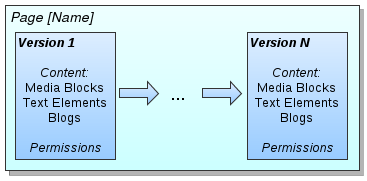
\includegraphics[width=0.7\textwidth]{CH6-F2-Version}
\caption{Page version control}
\label{fig:version}
\end{figure}

Creating a new version of an item is triggered by users on demand and is not
done automatically every time user alters or saves the item. This allows users to
control what they want to save and when.

As can be seen from the requirements in Table \ref{tab:req1}, this feature was
implemented for the \ep~pages. It was considered sufficient to demonstrate the
general concept as \ep~pages could be shared with others, and experience of
using this feature can be easily transferred to other shareable resources.

The component does not perform an automated difference analysis between versions
because pages can incorporate both textual and block elements that would make it
technically difficult and time consuming to implement this kind of analysis.
Therefore, analysing the difference between versions was left for users.
 
Adopting version control elements in \ep~system was expected to provide support
for communication and feedback-response cycle between students and lecturers, as
well as between students and audience outside of institutional environment.

\subsection{Concept Mapping Module}
\label{sec:mapping}
Addressing the challenges of \ep~knowledge management\footnote{In this thesis,
the \ep~knowledge management is referred to in terms of creating knowledge,
sharing it, managing and organizing it in \ep~space.} and development of
graduate attributes was a complex problem which required a creative approach and
no clearly suggested solution from the stakeholders. While looking at the other
areas for potential solution, it was discovered that qualitative data analysis
and knowledge visualization using concept mapping tool have properties suitable
for \ep~domain. Like \ep~work, qualitative data analysis is characterised by
rich data sets, opening the possibility of borrowing well established
techniques. Concept maps had potential as a supporting tool for organizing these
data sets into concepts and visualising them in a way that could be understood
by relevant audiences.

This section describes how bringing these two techniques together helped to
develop a solution for the problems outlined earlier.

\subsubsection{Parallels to qualitative research}

An \ep~can be called a container whose content needs to be organized, with
students not always knowing which items to select and where the items they put
in their \ep~should go. Students start their \ep~work by collecting \textit{raw}
data available from formal learning and outside activities and transforming it
into information that they decide to put into their \ep. After working with and
reflecting on this information students arrive at knowledge. However, sometimes
there is just too much data for students to cope with efficiently as they might
be initially lacking organizing skills. In this case, an \ep~system could
provide supporting solutions to help students manage their data.

A parallel with qualitative data analysis can be drawn here where researchers
either develop new theories from data, moving from specific observations to
general concepts and theories (inductive approach), or they try to check if
their data map against the theories that are already known and understood
(deductive approach) \citep{Strauss2008,Patton2002}. An assumption here is that
analyzing one's own learning process takes similar steps as qualitative data
analysis: small bits, specific data that learners are collecting, contribute to
the bigger picture of knowledge development. 

The difference is that the learner developing their \ep~is not aware of the
existing theories yet. These theories are the concept structures that exist in
the understanding of society, institution and employers. However, these must be
eventually understood and \textit{made their own} by the learner. Like the
qualitative researcher, the learner needs to immerse themselves in their data
and to come to an understanding of the kind of material they should be
collecting in their \ep~and the concepts that express their learning goals. They
need to find (and to a certain degree construct by exposing themselves to
learning opportunities) evidence in their data to show that they conform to
these concepts.

In qualitative research, a number of techniques are available to the researcher
in managing, analyzing and interpreting their data, such as coding, grouping,
generating categories and themes, rearranging and sorting \citep{Marshall2010}.
To support these techniques, specialized qualitative data analysis software
(QDAS), like
NVivo\footnote{\url{http://www.qsrinternational.com/products_nvivo.aspx}
(Accessed April 16, 2012)} and MAXQDA\footnote{\url{http://www.maxqda.com}
(Accessed April 16, 2012)}, has been developed which largely allows coding,
linking and mapping unstructured information. Although, QDAS could provide
students with necessary functionality for data analysis, it cannot substitute
the role of an \ep~system in the learning process. Reasons for that are outlined
in Table \ref{tab:qdas}.

\begin{table}[htb]
  \setlength{\abovecaptionskip}{0pt}
  \caption{Conceptual difference between QDAS and \ep~system}
  \begin{center}
    \begin{tabular}{| p{6.5cm} | p{6.5cm} |}
    \hline
     \multicolumn{1}{|c|}{\textbf{QDAS}} &
     \multicolumn{1}{c|}{\textbf{\ep~system}} \\
     \hline
     Do not share the analysis data & Showcase parts of the \ep~content to
     others \\ \hline 
     Only intermediate steps/data are contained, the research findings are
     written and communicated outside the system & Reflections, pages and data
     are apart of the \ep \\ \hline 
     Produce a report as an end point of the research  & Does not have an end
     point; data is constantly evolving; old concepts are changing and new are
     emerging with changing understanding of these concepts \\ \hline
    \end{tabular}
  \end{center}
  \label{tab:qdas}
\end{table}

However, the strength of QDAS is in how it allows to work closely with data.
Researchers \textit{label} data with codes, not just in order to connect these
labels later, but as an opportunity to \textit{dive} into their data by
re-reading, listening or watching it over and over again. This strength is
important for students as they need to revisit their material as their
understanding of concepts grows.

Currently, the majority of \ep~systems allow tagging their content with
user-defined tags. However, according to the results of interviews with
students, tagging does not provide necessary meaning to the \ep~data,
cannot show relations between concepts and does not allow building a flexible
structure. To address this problem, concept mapping was introduced into
\ep~environment to help students to be able use the same techniques available in
qualitative data analysis to manage unstructured data and develop learning
concepts in their \ep.

\subsubsection{Concept maps}

\citet{Mcaleese1998} formally defines a concept map as a directed acyclic graph
that consists of a set of Concept Labels and a non-empty set of Relationships
between Concepts. Putting it simply, concept maps are graphical representation
of the hierarchy of knowledge concepts and connections between them
\citep{Novak2008}.

Concept maps fit well with the qualitative data analysis techniques, outlined in
the previous section, as they are dynamic, process-oriented and give learners an
opportunity to engage in the learning process \citep{Mcaleese1998} which is
important for \LLLs \citep{Schuetze2006,Divjak2004}. Maps are created over time
by the learner who is engaged in a process of reflection, collecting and
selecting appropriate examples of their work. With concept maps, learners can
interpret their personal knowledge and map this knowledge and individual
examples against the existing theories. The hierarchical nature of the concept
map allows for organizing concepts from the high level abstract concept to the
more specific concepts. This property can be used by students for managing and
structuring data in their \ep s. 

In addition to the conclusions drawing from comparison with qualitative data
analysis, support for utilizing concept maps also comes from the literature.
While describing future directions for \ep~technology, Cambridge
\citeyearpar{Cambridge2010} suggested that visualization in the form of concept
maps could be a potential way of generating reflections.

QDAS already offers tools similar to concept maps in form of textual hierarchies
of nodes/terms/labels/concepts or as diagrams that show relations between
labels. Adding concept maps functionality to an \ep~system might make it
possible to borrow well established techniques of qualitative data analysis and
help students, who are analyzing their learning, to formally do what QDAS
already does informally. 

Concept maps have been already successfully used to in education to communicate
complex ideas, assess understanding of learning objectives, elicit knowledge and
provide conceptual frame for learning \citep{Novak2010}. A complete review of
the concept maps is beyond the scope of this thesis. For detailed examples and
evaluation of effectiveness of this tool refer to The Institute for Human and
Machine Cognition research group report \citep{Canas2003}.

\subsubsection{Component implementation}

The component (Figure \ref{fig:mapping}), presented in this section, adopts the
idea of concept maps in terms of developing or understanding concepts and
relations between them. Following qualitative data analysis techniques, students
create their own codes for the concepts which later form a concept map. Students
can also be provided with a map structure predefined by universities as a set of
Graduate Attributes in form of abstract concepts. Going thought the program of
study, students can learn to understand these concepts and recognize the
valuable examples of their work in the learning process.

\begin{figure}[htb]
\centering
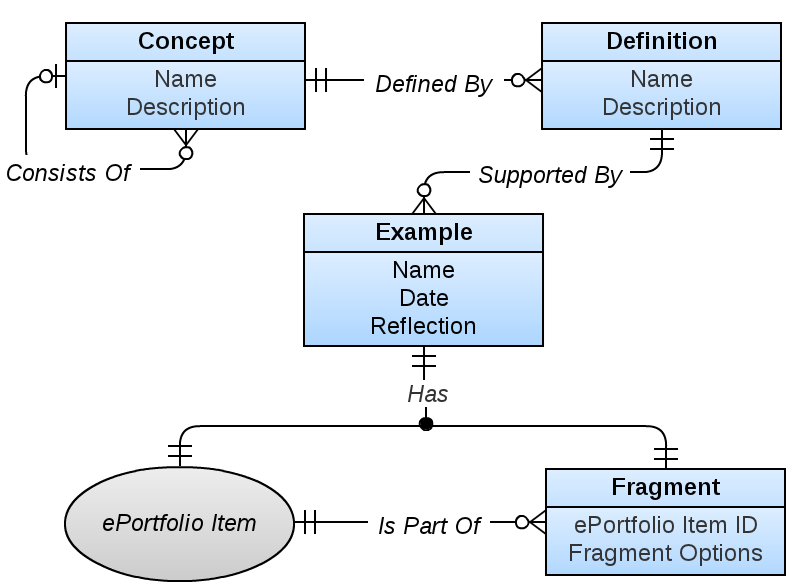
\includegraphics[width=0.7\textwidth]{CH6-F3-Mapping}
\caption{ER diagram of the concept mapping elements}
\label{fig:mapping}
\end{figure}

Using a \textit{tree} is considered to be the commonly used and natural way
of visualizing hierarchical data \citep{Gorg2007,Holten2006}. Trees are more
visually appealing, easier to master, and since trees are hierarchical, they are
better understood by many people. According to \citet{LeGrand2006}, they are
also easier to interpret than graphs. Therefore, instead of implementing a
complete directed acyclic graph structure, as described in the previous section,
concept mapping in this component was simplified to a tree-like structure and
did not provide cross-linking between the concepts.

Each map starts with an abstract core or key concept followed by optional
supporting sub-concepts. Hierarchy of the concepts can go as far as required by
learners starting from highly abstract concepts and going to very specific ones.
As shown on Figure \ref{fig:mapping}, students can provide definitions for the
concepts, which gives them descriptions from learners' point of view. As it was
noticed from the interviews with the stakeholders, often students do not
understand the meaning of the concepts offered by the university in the graduate
profiles or attributes. In this case, being able to provide own definitions to
the concepts, might help learners to express their own understanding and
communicate it to others.

Examples chosen by students for the concepts and definitions represent their
personal experiences and achievements. These examples are the fragments of
items, or entire items, from the \ep~repository. A detailed description of this
feature can be found in Section \ref{sec:frag}.

\begin{figure}[htb]
\centering
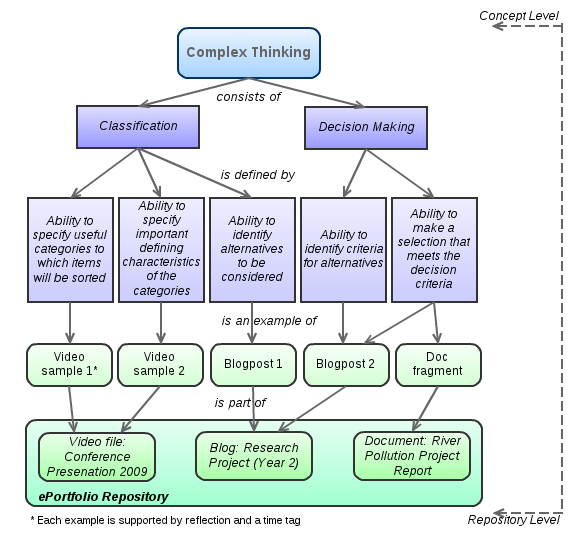
\includegraphics[height=0.5\textheight]{CH6-F4-Map-Example}
\caption{Concept mapping framework applied to the example}
\label{fig:mapex} 
\end{figure}

An \ep~concepts structure can be represented as shown in Figure \ref{fig:mapex}.
Data for the example was taken from the examples offered by \citet{Marzano1993}
on how to assess \LLLs standards.

Due to the dynamic nature of learning process, this kind of structure might
never be complete. It is constantly changing as students deepen their
understanding and potentially find more suitable evidence to underpin their
development.

\FloatBarrier

The expectations are that this approach would allow students to:
\begin{itemize}
  \setlength{\parskip}{0pt}
  \setlength{\parsep}{0pt}
  \setlength{\itemsep}{2pt}
  \item Manage and structure large amounts of information in their \ep:
  students will be able to organize and navigate through the information, find
  relations between the content and the concepts and see the data in their
  \ep~from various perspectives: from an item belonging to different
  structures; from a concept containing multiple evidences; and from items and
  concepts attached to a timeline (Section \ref{sec:timeline});

\item Share their progress/development map with others for feedback or
evaluation: students will be able to create specific structures for various
purposes to show to the audience specific parts of their \ep~(for example,
share with a potential employer communication and writing skills developed over
the last year at university);

\item Access and address institutional graduate attributes: by providing
students with a concept map of the graduate attributes (maybe even already
supported by the institutional definitions), universities would be able to
help students to understand the skills requirements of their study area and look
at their study program from the \LLLs perspective;

\item Develop a flexible structure for self-directed learning: students are
provided with all operations necessary to make their structures flexible such as
creating new concepts, removing or merging existing ones, creating links between
structure fragments and taking snippets of \ep~items as examples (Section
\ref{sec:frag});

\item Facilitate setting up learning/development goals and expressing students
visions of their knowledge: constructing their own concepts and definitions
might encourage students to think of what skills are important to them, how they
understand these skills and how it links to their learning outcomes.
\end{itemize}


\subsection{Artifacts' Fragments Extraction}
\label{sec:frag}

Artifact's fragments extraction was developed as a part of the concept mapping
module. This feature allows selecting \ep~artifact's fragments and using
them as example in definitions of the concepts described in the previous
section.

The idea behind this feature was to allow students to share specific parts of
\ep~artifacts linked to the conceptual level of their learning. Because
extracting a fragment is a part of creating an example to the concepts, each
fragment has to be supported by the student's reflection. Reflection should
explain what is so special about this example, or how it addresses some specific
concept which it refers to. It is expected to help students understand that
their \ep~space is not a place for \textit{dumping} all possible items. Each
element of an \ep~is an important example of their personal and professional
development carefully selected to showcase learning progress.

When learners create a fragment as a part of an example, they can link it
directly to the concepts that already exist in their \ep. In case learners do
not know where this example belongs to in the hierarchy of concepts, they can
leave it as a free fragment and use later.

To demonstrate this feature, the following artifact fragments were implemented:

\begin{itemize}
  \item Image: JPEG, PNG, GIF -- by selecting of a part of an image;
  \item Video: OGV, MP4, 3GP, WEBM -- by specifying start and end time of a
  fragment;
  \item Text: TXT -- by selecting a text fragment;
  \item Blog -- by selecting one or more blogposts;
  \item Bookmark: URL of the resources on the Internet -- no selection is
  required.
\end{itemize} 

Figure \ref{fig:frag} shows the way of extracting fragments for various
\ep~artifacts.

\begin{figure}[h!]
\centering
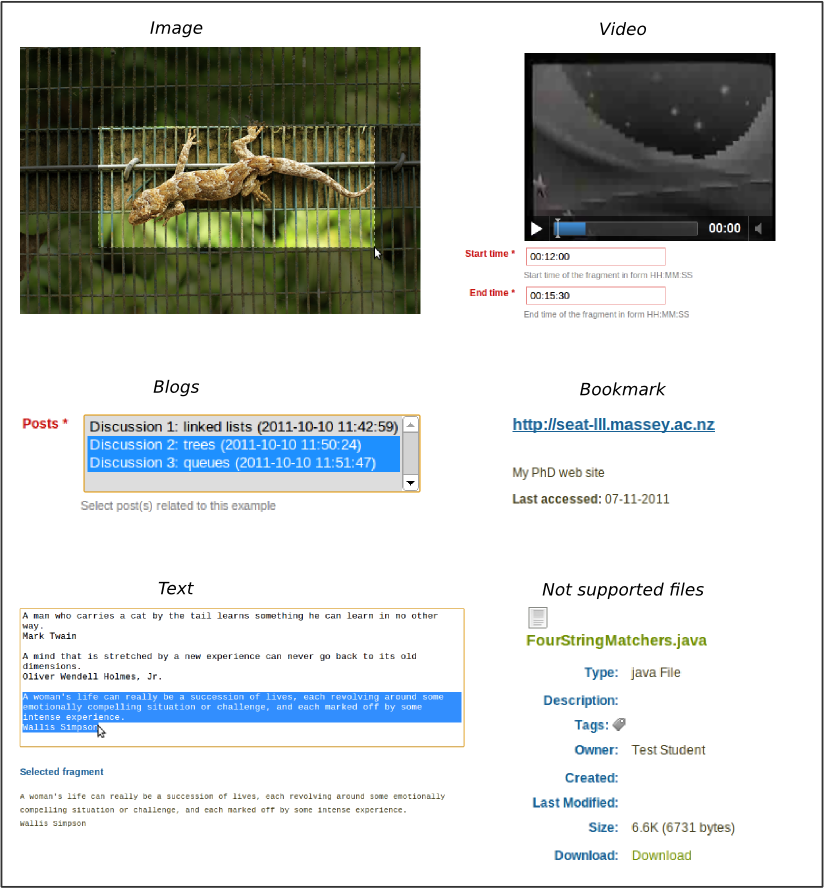
\includegraphics[width=0.99\textwidth]{CH6-F5-Fragments}
\caption{Artifact's fragment extraction}
\label{fig:frag}
\end{figure}

\FloatBarrier

At this stage, fragments of textual files support only TXT files because
popular, but proprietary formats as PDF or DOC do not allow selecting fragments.
Although it is possible to access specific fragments of PDF documents through
fragment identifiers, it is not possible to extract the fragment and restrain
access to this fragment only.

Files that do not support fragments extraction allow attaching an entire
artifact for download. Each extracted fragment can be as well accompanied with a
link to the item in case learners would want to allow its download.

Using fragments of artifacts can be useful for a number of reasons:
\begin{itemize}
  \item it allows to draw attention to a specific part of artifacts (like part
  of a picture, or fragment of a video);
  \item it allows the presentation of different parts of artifacts to different
  audiences;
  \item it helps to avoid files duplication;
  \item it saves user's time that otherwise would be spent on cropping images,
  videos, or textual files;
  \item it can help to solve some ethics issues (for example, students studying
  to become teachers are not allowed to show the faces of children they teach at
  schools, but they still have to demonstrate their competencies of teaching).
\end{itemize}

From the perspective of this component evolving Media Fragments 1.0
specification \citep{MediaGroup2011} becomes very useful as it describes the
ways of extracting temporal and spatial media fragments using Uniform Resource
Identifiers (URI). Once it is finished (as planned for December 2011 -- January
2012), this specification could be adopted in the \ep~system for improved
fragments description and extraction.

\subsection{Learning Progress Tracking}
\label{sec:timeline}

Timeline representation of learning progress was developed in conjunction with
concept mapping component. It is used to present the data from the concept map
in chronological order.

Timelines are used in various areas, such as education, history, natural
sciences, software development and project management, for presenting and often
visualizing a progression of related events. This valuable property of a
timeline to show progression was used in the prototype development to bring a
sense of change over time to the learners analysing their personal or professional
development.

Timelines in the prototype are generated automatically and do not require
user's input. Each example described in the previous section is accompanied with
a \textit{time tags} whether is it taken from the properties of the artifact as
creation date or added as a customary selected date. These time tags of the
examples allow any concept map to be transformed into a timeline, as shown on
Figure \ref{fig:timeline}. Each entry on the timeline is an example from the
concept maps.

\begin{figure}[htb]
\centering 
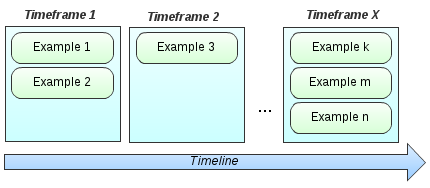
\includegraphics[width=0.75\textwidth]{CH6-F6-Timeline}
\caption{Timeline structure}
\label{fig:timeline}
\end{figure}

Standard representation of the timeline uses a linear time scale available in
two options, i.e., month and year. In addition to the standard representation,
users can create their own time scales with the custom time frames (e.g., BA
year 1, BA year 2). In custom time frames, users need to specify start and end
date of the frame. Examples are then grouped and visualised under a specific
time frame based on their time tags. 

Users can navigate through any part of the timeline by clicking on the bar
labeled with time frames. Clicking on the entry brings up a window with the
details of the example: title, reflection and concept it belongs to.

Information on the timeline can be filtered based on the concepts hierarchy of
the map. This can be used to see the progress towards development of some
specific concept(s), changes in feedback and improvements of the examples.

Adoption of this component is expected to provide support for tracking personal
progress in various areas and aspects. Generating timelines could add a temporal
dimension to students progress analysis: they would be able to see how their
skills evidence changed with time, how feedback received from the others
reflects their growing understanding, what achievements they have made and what
concepts require more input. It could also help to showcase the progress for
evaluation or share it with others for feedback purpose.

\subsection{Shared Resources Management}
\label{sec:sharing}

To be able to share the parts of \ep~in a way required by the stakeholders was
another important aspect of \LLLs support that needed improvements. As was shown
in the previous chapters, current \ep~systems already provide extensive list of
sharing options: by email, secret URL, temporary accounts, etc. However,
managing shared resources was missing from the features provided by these systems.

The following improvements were implemented in this area to provide a better
control over shared resources:

\begin{itemize}
  \item Saving sharing/access history: every time a page or a concept map is
  shared with others a record is created in the user access log. This allows the
  user to review when a part of \ep~was shared and with whom; 
  \item Easy re-share through access history: Saving access history made it
  possible to re-share resources with the same audience once their access
  expires;
  \item Notifications on access expiry for system users and resources shared by
  email: if set up by a learner, when access to the shared resources is close to
  the expiry date, the system sends notification to people on the access list;
  \item Control over level of feedback provided: bringing concept mapping with
  its hierarchy of concepts and examples into \ep, opened opportunity to give
  learners control over level of feedback they expect to get. In concept maps,
  learners can choose what kind of feedback they want, whether it is feedback on
  overall map structure, individual examples or a group of examples related to a
  concept. From lecturers' perspective, it allows them to attach their feedback
  to the elements of a concept map which means that they can focus on specific
  aspects as well as on the general picture.
\end{itemize}

Better control over shared resources has potential to bring more confidence to
learners, support dialog between interested parties, improve quality of
feedback, and facilitate its provision in a timely manner.

\section{Prototype Iterations and User Tests}
 
Before formal evaluation was undertaken, implemented functionality had been
reviewed by users. Overall, despite time and resources constraints of the
project two prototype iterations were possible. Each iteration produced a
workable version of the implemented features. At the end of each iteration, the
functional prototype was presented to a student and a lecturer selected from the
participants of the requirements elicitation phase who had agreed to continue
their participation in this research.

Each feedback session included up to an hour demonstration and discussion of the
implemented functionality. Users were encouraged to give their ideas about
additional improvements and provide their thoughts on possible drawbacks of
presented implementations.

Feedback between iterations was very useful as it facilitated further discussion
with the stakeholders and helped to get more information on potential
improvements. Users were generally satisfied with the improvements and made
largely positive comments. However, several issues were noticed. Most notably,
users mentioned that they would have difficulties using the system on their
own without comprehensive instructions. Some features not common for web
interfaces, like right-click context menu in concept mapping, might confuse
novice users. It was decided that starting tips on the web-pages could be an
additional help to the beginners who are not familiar with the system.

All discovered issues were addressed in the later versions of the prototype
in preparation for the formal evaluation stage.

\section{Summary}

This chapter presented design and implementation of additions and improvements
of the \ep~system based on the needs of the stakeholders and \LLLs success
guidelines discovered in the literature. A set of features was introduced to
the standard \ep~installation with the aim to address various aspects of \LLLs
support in universities. These features are expected to support understanding,
development an showcasing of \LLLs skills, learning progress tracking,
management of \ep~content and knowledge, communication between students and
lecturers, and better control over access to the \ep~resources.

From this stage, to understand whether new implementations meet the needs of
the stakeholders, a formal evaluation has to be undertaken. The next chapter
looks at the improved \ep~system prototype from the perspective of lecturers
and students with various levels of experience.
 
\chapter{Evaluation\label{cha:evaluation}}
%10500
Throughout this thesis the requirements, design and prototype implementation of
the \ep~system that can support \LLLs has been discussed. This chapter focuses
on the evaluation of this research and its contributions based on three studies.
The studies were designed to look into the specific aspects of \LLLs support and
understand how well developed features satisfy the requirements identified
earlier by the lecturers and students. 

The number of studies represents perspectives of all of the stakeholders that
have been involved in this research earlier, i.e., lecturers and students.
Reason for this was to ensure that all of the perspectives are being captured as
\textit{different stakeholders often have different perspectives}
\citep[p.~111]{Hevner2010}. In addition, the evaluation from the students'
perspective has been split into two studies as the requirements elicitation
stage discovered that the perception of \LLLs depends on the maturity of
students. Therefore, it was decided to use different evaluation approaches for
each group of students.

The first section of this chapter describes the approaches and data collection
methods used in the evaluation stage. Further, each of the three studies is
presented with the detailed participants profile description, exercise protocol
followed by the study, artifacts collected and the results of data analysis.
Each study section ends with conclusions that look into recommended improvements
to the \ep~system prototype and its processes.

\section{Design Overview}
As this chapter aims to evaluate this research and its contributions, the
relevant research question and its sub-questions are restated here:

\textit{How does the extended environment meet the needs of the stakeholders in
university teaching and learning contexts?}
\textit{\begin{itemize}
  \item How can lecturers use new features to provide students with their
  guidance and help them to understand \LLLs skills?
  \item How can students address \LLLs skills using new features?
  \item How can new features help students track their learning progress, manage
  \ep~knowledge and organize content, demonstrate and share their
  achievements with others?
\end{itemize}}

To answer these questions, three studies were carried out independently from
each other. The results were used to evaluate the developed prototype from three
different perspectives: lecturers, mature students and less experienced
students. Each study followed its own exercise protocol described in the related
sections. Detailed design of each study can be found further in this chapter in
Sections \ref{sec:one}, \ref{sec:two}, and \ref{sec:three} respectively.

Data collection for analysis was performed using both quantitative and
qualitative methods to support the principles of multiple sources and multiple
perspectives of data advocated by many researchers
\citep{Yin2009,Maimbo2005,Marshall2010}. The following techniques were used over
the course of all studies:

\begin{itemize}
  \item Behavior observations made by the researcher during all studies.
  \item Observation data in form of digital photographs taken during the group
  experiments.
  \item Audio recordings of the face-to-face interviews collected to facilitate
  more thorough interview analysis.
  \item Open-ended questions asking for participants opinion on the features and
  tools used in the studies.
  \item Close-ended questions that required participants' evaluation based on
  ten point scale, from \textit{not useful at all} to \textit{highly useful}, 
  included in exit questionnaire.
  \item Physical artifacts in form of paper records made by participants of the
  group experiment.
  \item Digital artifacts in form of electronic records in the \ep~system made
  by participants of the group experiment and case studies.
  \item System logs demonstrating \ep~system use by case study participants.
  \item Additional evidence, comments and opinions collected by the researcher
  through informal discussions that would help to support analysis and
  conclusions.
\end{itemize}

Audio recordings as well as digital photographs were collected with the
permission of the participants and performed without interrupting the process of
each study. More detailed description of data collection methods for each study
can be found in the relevant sections this chapter and associated appendices. 

\section{Evaluation Limitations}

It is important to remind here that in the context of this thesis, it is
impossible to fully evaluate \LLLsn. Ideal evaluation would include providing
students with a technical support solution developed in course of this project
and monitoring their activity through the years of studying at the university.
However, this approach appears to be not feasible due to the nature and scale of
this research project, its time and resources constraints. No existing
evaluation design has been found that would suggest an acceptable approach.
Therefore, the evaluation stage in this project followed its own design that
attempted to explore and analyse the implementations from the perspective of
the \LLLs stakeholders.

\section{Ethical Considerations}

Similarly to the earlier stage of the requirements elicitation, the Massey
University Ethics Approval process was followed for the evaluation studies of
this research. Analysis of the evaluation design with the Human Ethics Chair
concluded that none of the three studies required full ethical approval.
Therefore, a ``Low Risk Notification" was submitted to the Massey University's
Low Risk Database.

Ethics documentation, such as the Ethics Approval Letter, student information
sheets and participant consent forms, used for this research project stage, can
be found in Appendix \ref{cha:app5}.

\section{Study One. Exploratory Evaluation by Lecturers}
\label{sec:one}

To achieve the ultimate goal of this research project to develop a system that
can provide support for \LLLs in universities, it is important that learning
facilitators, e.g. lecturers, could successfully utilize improved technology to
help and guide students in their learning journey. Therefore, this study
explores the prototype implementations from the lecturers' perspective to
understand whether their initial requirements were met.

\subsection{Goals}

The goal for this study was:

\smallquote{To find out whether lecturers can use new features to provide
students with their guidance and support, and help them to understand \LLLs
skills.}

To support achievement of this goal, the main objectives were:

\begin{itemize}
  \item To evaluate whether new features can provide better communication
  opportunities between lecturers and students;
  \item To determine how lecturers can use new features to help students
  understand the link between \LLLs skills and their university degree study;
  \item To explore how lecturers can utilize new features in the classroom to
  guide students through development of \LLLs skills. 
\end{itemize}

\subsection{Research Protocol}

This study was an exploratory study that used a demonstration and participants
interviews as a research evaluation approach. According to \citet{Peffers2008},
\textit{demonstration} is normally used to show that idea works and precedes a
more \textit{formal} evaluation. In this research project, demonstration was
included into the overall evaluation design. The expectation was that in
combination with the participant interviews, followed after each demonstration,
it would provide a valuable insight into the lecturers' perspective on the
prototype features.

For the purpose of this study, six one-on-one interviews and one small group
discussion were organized with the participants. Group discussion was undertaken
during the annual staff meeting and involved three participants.

This study did not follow a strictly defined research protocol as the directions
of the meeting discussions were based on the outcomes of the semi-structured
conversations with the participants. Each meeting started with the brief
introduction of the research and the purpose of the demonstrations undertaken.
To guide the course of the study, the researcher initially had a set of topics
to cover in the presentation and demonstrate the prototype functionality with
the examples of how it could be potentially adopted in the learning environment.
The discussion topics were based on the implemented features described in detail
earlier in Chapter \ref{cha:prototype}.

Each of the topics was presented to the participants in the following order:

\begin{itemize}
  \item the problem addressed in the topic;
  \item an implementation suggested to solve the problem;
  \item a step-by-step demonstration of how this implementation works in the
  \ep~system;
  \item expected/intended use of the feature in the classroom;
  \item where possible, examples of use in the \ep~system.
\end{itemize}

After the demonstrations, the participants were asked to assess the prototype
features based on their personal and professional experience. From their
perspective they evaluated whether the presented scenarios of use were realistic
and what challenges they could see in the suggested ways of using the features.

The lecturers were then asked to suggest how they would use new features and how
they would apply the methods these features incorporate with their students. At
the end of the topic discussion, the participants were offered to recommend the
potential improvements.

All interviews were audio recorded and transcribed for the purpose of more
thorough analysis. Direct citations in the results section (Section
\ref{sec:study1results}) were taken from the interviews transcripts.

\subsection{Participant Profiles}

This study used a number of techniques to identify suitable participants.
Initially, each of the lecturer-participants of the previous stage of
identifying requirements for \LLLs supported by \ep~systems was offered to take
part in the evaluation of the prototype implementations at the later stages of
this research. Three lecturers expressed interest in continuing their
participation in the project.

The rest of the participants were recruited using snowball sampling strategy
which had already been employed earlier in this research. This strategy relied on
recommendations of the existing participants having knowledge of the suitable
candidates who would potentially be interested in this research. Based on
criteria of being a lecturer or having previous lecturing experience, and
also having experience of using an \ep~system with the students, six other
participant were identified from the suggested candidates.

Overall, the data was gathered from nine participants, all lecturers at
various schools and colleges of Massey University. Table \ref{tab:study1part}
shows demographics of the participants:

\begin{table}[htb]
\setlength{\abovecaptionskip}{0pt}
\caption{Demographics of the Study One participants (n = 9)}
  \begin{center}
    \begin{tabular}{| l | c |}
    \hline
     \multicolumn{1}{|c|}{\textbf{University Structure}} &
     \multicolumn{1}{c|}{\textbf{Number}} \\ \hline
		College of Science: & \\ 
		-- School of Engineering and Advanced Technology & 1 \\
		-- Institute of Veterinary, Animal and Biomedical Sciences & 1 \\
		-- Institute of Food, Nutrition and Human Health & 1 \\ \hline
		College of Education: & \\ 
		-- School of Curriculum and Pedagogy & 2 \\
		-- School of Educational Studies &  3 \\ \hline
		Centre for Teaching and Learning & 1 \\ \hline
	\end{tabular}
  \end{center}
\label{tab:study1part}
\end{table}

One of the participants was a program coordinator for a Bachelor degree program
and had a particular interested in how the prototype functionality can be used
with the university graduate attributes and \LLLs skills.

The lecturers from the College of Education had the most experience of using
portfolios or \ep s with their students. The reason for this was that every
potential teacher in New Zealand had to meet the requirements developed by the
New Zealand Teachers Council in form of Graduating Teacher
Standards\footnote{\url{http://www.teacherscouncil.govt.nz/te/gts/}}. These
standards closely resemble university graduate attributes and \LLLs skills.
Teaching portfolio has to be created by students as a proof that they meet these
standards. The College of Education lecturers were at the earlier stages of
adoption of the institutionally supported \ep~system for these purposes and
therefore were highly interested in giving their feedback on the prototype
implementations.

A representative of the Centre for Teaching and Learning was considered a
suitable participants as they had previous teaching experience, both at school
and at university, and at that time was assisting adoption of the new learning
technologies, \ep~systems in particular, in the university courses.

Each participant was approached by an invitation email to take part in this
research and evaluate the developed features in a face-to-face meeting with the
researcher.

\subsection{Results}
\label{sec:study1results}

In general, feedback given by the lecturers based on the demonstrations was
positive.

Concept mapping \ep~module with all adjacent to it features such as
artifact's fragment extraction, timeline progress tracking and sharing
opportunities raised the most interest among the lecturers.

Some lecturers looked that the demonstrated features from the assessment
perspective. Version control in the \ep~system was found useful for giving
better feedback to student and tracking their responses as well as progress.
Concept maps was called a tool for more rigorous assessment of students'
understanding of the concepts they have learnt. Some of the lecturers had been
using mapping techniques for assessment of their students' knowledge before and
said that having the tools that could support concept mapping in the \ep~system
would be very useful.

From another perspective, as was described by the lecturers, students might
be interested in using the new concept mapping tools for two reasons: to
communicate what they have learnt to somebody else or to try to make sense of
the things that they are learning at the moment.

One lecturer said that they liked concept mapping module in particular for its
potential to provide support for both horizontal and vertical integration of
knowledge and skills. Integrating the knowledge of their study degree as well as 
bringing together the things that students learn from other subjects is very
important:

\shortquote{What I like about this tool is that at the end students should be
able to clearly see how everything is built towards them achieving these
[graduate] attributes or not.}

However, stepping away from discussion of implementations, another participant
noticed that the problem with the new tools might be that students are less
likely to use them \textit{``for their own good''}. Therefore, an element of
assessment might be required at first. In this case, it becomes an exercise that
needs to be completed which is not the same thing as using system on learner's
own motivation.

Two of the participants mentioned that, before making any serious decision
whether the demonstrated features are feasible for use with students, they would
like to hear their opinion on these features:

\shortquote{I can see some opportunities for what we are trying to do in the
future. I definitely see potential. However, to be sure, I would be interested
in the students try to use these tools and tell us how they see it.}

The group meeting with three lecturers from College of Education had the most
active discussion of the implementations compared to one-on-one interviews
with other participants. These lecturers just finished their first trial with
the students where they were using an institutional \ep~system for creating
students' teaching profile. As a result, they had most recent experience with
students using an \ep~system to support \LLLsn.

According to the feedback given, the following are the attributes of the
implementations that the participants of the group meeting liked most of all:

\begin{itemize}
  \item Visual nature of concept mapping;
  \item Simplicity of making complex things;
  \item Challenge of conceptual understanding;
  \item Authentic evidence that students meet the outcomes;
  \item Opportunity for various levels of feedback;
  \item Ability to draw attention to the specific elements with fragment
  extraction;
  \item Ability to see students' progress towards learning goals.
\end{itemize}

Along with the positive features, a number of potential challenges were noted:

\begin{itemize}
  \item Not only students, but lecturers as well require training on how to
  use new systems and new features in their classroom:
  \shortquote{Teachers need training too. We used to think that teachers know
  everything and know how to bring new technology to their classroom. But in
  reality, they don't.}
  
  \item Students need assistance throughout the process of learning the
  \ep~system: 
  \shortquote{We have all sorts of students and not all of them are on good
  terms with technology. Some struggle with such simple things as writing a
  blog or creating a web page, even when they have all the instructions
  required. If you want this system to be accepted by students, they need to be
  sure that help is always out there for them.}
  
  \item Curriculum should be adjusted to support \LLLsn:
  \shortquote{Our challenge is to develop the notion of \LLLs ability and what
  it means for that to be a good practicing [engineer, lawyer, doctor]. And we
  need to embed it early on, because they [students] don't know the notion at
  the moment.}
\end{itemize}

It is also important to mention that after the formal part, five out of nine
participants asked when they could expect to see the demonstrated features in
the official release of the \ep~system that they had been using in the
university and expressed willingness to include these into their work with
students. Arguably, this can be considered as an indicator of value and
usefulness of the developed features recognized by the participants during the
demonstration.

\subsection{Conclusions}

Overall, the outcomes of Study One were very useful and provided a valuable
first-hand evidence reaffirming that the lecturers were satisfied with the
developed features and their requirements of the earlier project stage
implemented in the prototype had been met.

Although, no potential improvements were recommended by the participants, a
number of challenges of using prototype feature to support \LLLs were
identified: need for training of lecturers, providing support for students, and
adjusting study programs to develop the notion of \LLLs ability.

Based on discussions during the demonstrations and the interviews with
participants afterwards, it can be concluded that the prototype features were
well accepted and raised a high interest among the lecturers. However, it can be
also seen that at that stage one of the important things for the lecturers was
to ensure that students themselves see these features as positive which
required further evaluations of the prototype.

\section{Study Two. Group Experiment -- \LLLc Skills Development and
Demonstration}
\label{sec:two}

This study investigates students perception of the concept mapping tools as a
part of the \ep~system in terms of constructing and sharing knowledge,
understanding and demonstrating achievements, and linking practical experiences
to the conceptual skills.

\subsection{Goals}
The goal for this study was:

\smallquote{To find out whether undergraduate students find concept mapping embedded
into the \ep~system helpful in terms of addressing graduate attributes, learning
objectives, and \LLLs skills and tracking their progress in learning.}

To support achievement of this goal, the main objectives were:

\begin{itemize}
  \item Determine whether concept mapping embedded into the \ep~system provides
  students with a suitable tool for addressing graduate attributes and \LLLs
  skills;
  \item Investigate whether the process of development of concept maps
  influences students' understanding of personal learning achievements and
  skills that they learn during degree program study;
  \item Determine whether concept mapping embedded into the \ep~system can be
  successfully used to demonstrate personal achievements and skills;
  \item Analyse how useful students' consider concept mapping methods as a part
  of the \ep~system.
\end{itemize}

\subsection{Research Protocol}

To ensure a better control over the experiment settings, it was conducted with
the small groups of students at a time (35 participants in total). All groups
followed the similar process outlined in Study Protocol in Appendix
\ref{cha:app6} with up to two hours for the entire experiment to complete. Time
of completion might have varied between groups due to the differences of the 
participants' previous experiences. For example, some of the students did not
require explanation of \LLLs concepts or tutorial on how to construct the
concept maps.

Work with each group of students began with an introduction to the research,
activities to be performed and an explanation of participants' rights.
Ethics documents, such as the information sheet and the consent form, were then
distributed. Signed consent forms to participate in the experiment had been
collected before any other activities and exercises were started.

The introduction included a brief overview of the research project, a
presentation on \LLLs concepts, demonstration of the \ep~system and examples of
use. Concept mapping as a method of constructing knowledge was discussed in
detail.

After the introduction part, each participant was provided with a pen and a
sheet of paper to work with the first exercise, examples of institutional
attributes and courses learning objectives, examples of concept maps, unique
access account to the prototype \ep~system, user manual for the \ep~system
concept mapping tool and artifacts fragments extraction, and exit questionnaire
sheet.

Second part of the experiment consisted of two exercises: the first one
performed on paper and the second one performed using the prototype \ep~system
tools. Between the exercises, students were given a demonstration of the
prototype functionality that allowed to construct concept maps in the \ep~system
and attach examples from the \ep~repository to the concepts. After the
demonstration, students proceeded to the second exercise. 

At the end of the experiment, all participants were asked to complete the exit
questionnaire to collect their evaluations and opinions on the tools and methods
they had just used.

Although, working independently during the experiment was highly encouraged,
students were allowed to do exercises in pairs or groups up to three students.
In case they were working in pairs, students still had to complete the exit
questionnaire independently.

\begin{figure}[htb]
\centering
\includegraphics[width=1\textwidth]{CH7-F7-Settings}
\caption{Experiment settings}
\label{fig:settings}
\end{figure}

Figure \ref{fig:settings} shows the settings in which the experiment was
performed. Standard university computer classrooms were used for the experiment.
Participants did not have allocated places which allowed them to choose more
comfortable settings for the duration of the experiment. The researcher was
available at any time during the experiment for assistance.

\subsection{Participant Profiles}

As was already mentioned in the previous section, thirty five students from
various undergraduate and graduate programs at Massey University agreed to
participate in this experiment. Table \ref{tab:degree} shows the wide range of
degree programs the students were enrolled in.

\begin{table}[htb]
\setlength{\abovecaptionskip}{0pt}
  \caption{Degree programs of the Study Two participants (n = 35)}
  \begin{center}
    \begin{tabular}{| l | c |}
    \hline
     \multicolumn{1}{|c|}{\textbf{Degree Program}} &
     \multicolumn{1}{c|}{\textbf{Number}} \\
     \hline
     Bachelor of Engineering & 2 \\ \hline
     Bachelor of Health Science & 1 \\ \hline
     Bachelor of Science & 3 \\ \hline
     Bachelor of Veterinary Science & 7 \\ \hline
     Graduate Diploma in Secondary Teaching & 14 \\ \hline
     Graduate Diploma in Primary Teaching & 7 \\ \hline
     Bachelor of Information Sciences & 1 \\ \hline
    \end{tabular}
  \end{center}
  \label{tab:degree}
\end{table}

All participants were volunteers recruited through the announcements in the
classroom of various courses in College of Education and College of Science or
through the poster invitation distributed through the lecturers at Massey
University.

As shown in Figure \ref{fig:demograph}, participants' age ranged largely from
twenty to thirty years which was expected as this experiment aimed at studying
undergraduate students. Gender distribution was relatively equal with fifteen
male and twenty female participants.

\begin{figure}[htb]
\centering
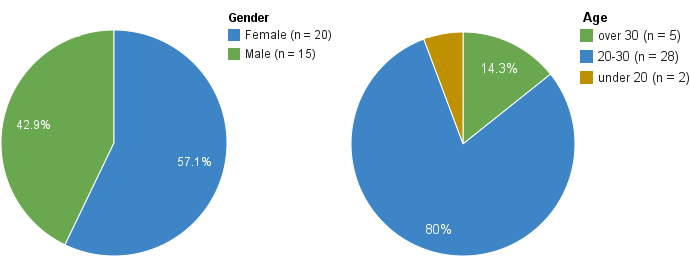
\includegraphics[width=1\textwidth]{CH7-F5-Demographics}
\caption{Participant demographics (n = 35)}
\label{fig:demograph}
\end{figure}

Twenty seven students reported that they were familiar with the concepts
of \LLLs before taking part in this experiment. However, only thirteen of these
twenty seven students said that they were familiar with the term
\textit{graduate attributes}. They were primarily Teaching Graduate Diploma
students form the College of Education. As was discovered during the informal
post-experiment discussion, this might be explained by the fact that College of
Education of Massey University uses term \textit{teaching profile} instead of
\textit{graduate attributes} to describe \LLLs skills and competences of the
degree program.

In the background section, twenty nine students said that they knew about
\textit{\ep} prior to the experiment. Seven of these students reported using an
\ep~system to demonstrate their \LLLsn. They were Veterinary Science students
who had \ep~work included into their degree program curriculum.

\subsection{Activities and Artifacts}

Figure \ref{fig:procedure} provides an overview of the experiment procedure and
the activities or tasks performed by the participants for each part, based on
the above described study protocol.

\begin{figure}[htb]
\centering
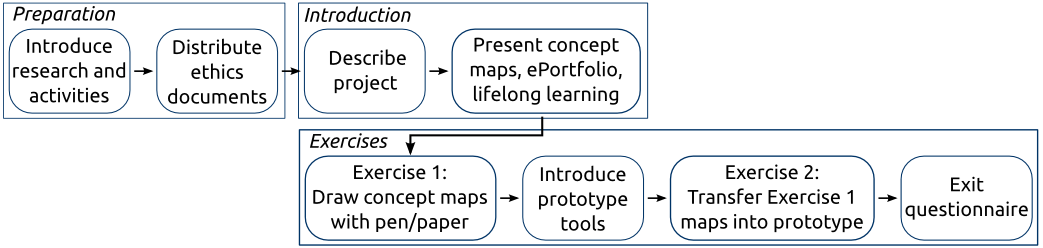
\includegraphics[width=1\textwidth]{CH7-F8-Activities}
\caption{Experiment procedure}
\label{fig:procedure}
\end{figure}

\FloatBarrier

Length of the presentations and information content of the introduction part
varied depending on the participants' experience.

List of the artifacts used by the students in this experiment was following:

\begin{itemize}
  \item Ethics documents: a) information sheet, and b) consent form;
  \item Pen and paper for the first concept mapping exercise;
  \item Examples of the institutional graduate attributes and courses learning
  objectives taken from the Massey University web-site;
  \item Examples of concept maps in the \ep~system created by the researcher;
  \item Instruction sheet with the unique access account to the \ep~system;
  \item User manual for the \ep~system concept mapping tool;
  \item User manual for artifacts fragments extraction;
  \item The exit questionnaire.
\end{itemize} 

Appendix \ref{cha:app6} provides samples of the documents used in the
experiment, such as the poster invitation to participate in this experiment,
study protocol followed, the exit questionnaire and the responses to it (Section
\ref{sec:responses}).

\subsection{Data Analysis and Results}

The data collected during this evaluation were based on exit questionnaire
results, observations and system records. These are described in the related
subsections of this section.

\subsubsection{Observed Behaviour}

Based on observations, the most difficult for students was the very beginning of
each of the exercises. In the informal discussion after the experiment, some
of the students admitted that having a blank sheet of paper or an empty
\ep~system account in front of them as they started was rather intimidating. At
first, students expected to be told what to draw and which concepts to include
into their diagrams. After a short explanation that there were no right or wrong
concept maps that could represent their own learning experience or skills, the
process of working with concept maps moved on.

All students were able to complete exercises in allocated time. Students, new to
the concept mapping, followed the techniques presented in the introduction
tutorial on how to build the maps. This included deciding the main message or
the key concept of their map followed by identifying the related concepts. When
this was done, they tried to organize the concepts into maps (Figure
\ref{fig:study2maps}, a).

% TODO: photo of the concept maps on paper
\begin{figure}[htb]
\centering

\includegraphics[width=1\textwidth]{CH7-F12-Map-Photo}
\caption{Concept map drawing examples by the students}
\label{fig:study2maps}
\end{figure}

More experienced students preferred to follow their own established procedure of
creating concept maps. Some of them did not spend time making a list of the
concepts, but were adding concepts straight to the maps making corrections when
necessary (Figure \ref{fig:study2maps}, b).

Due to the lack of information about previous experiences of the participants,
in some cases groups consisted of students with very different knowledge of the
discussed concepts. The problem with this situation was that while the students
with no experience required assistance, more experienced participants tended to
jump ahead of the group in doing exercises, following manual on their own and
not waiting for the demonstration of the evaluated functionality of the
prototype. At this stage, it is not possible to analyse whether this had any
influence on the results of the evaluation, as the demonstration which those
students would have followed, had the same information content as the user
manual on the prototype functionality. Therefore, it possible to assume here
that all participants worked under the same conditions.

\subsubsection{Exit Questionnaire Results}
The exit questionnaire responses were the major data collection source for the
user feedback and evaluation. The questionnaire consisted of two parts: Section
A (background information) and Section B (evaluation). The responses on Section
A have already been described in Participants Profile Section for this study. This
section will focus on the responses on Section B of the questionnaire. 

In the evaluation part of their exit questionnaire the participants were asked
various primarily open-ended questions aimed at understanding what kind of
experience they had working with the prototype and getting their feedback on the
tools and methods used during the experiment. Following the questions, the
students described their impression of using new \ep~features, considered the
impact that these features might have on their personal learning and while
addressing graduate attributes, indicated most and least favored elements in the
implementations, provided their measure of usefulness based on ten point scale
and suggested potential areas for the improvements.

In general, the responses were very positive. Comments made by the participants
during the exercises showed that they enjoyed the work with concept mapping
tools in the \ep~system. 

Based on the responses to the Section B of the exit questionnaire, students
found \ep~concept mapping to be a valuable experience. According to their
comments, the tools and methods that were used during the experiment helped
them to think about bigger picture of their learning, 

\shortquote{Most of all I like that it allows me to can see bigger picture of
my learning and developement.}

make links between the concepts they have learnt at the university, 
\shortquote{I think that being able to layout concepts in a clear structure like
you can here with definitions and examples would help to cement an understanding
of the significance of what a student has learnt in a specific subject and how
it links to other subjects.}

think how these concepts contribute to the skills development, 
\shortquote{It helps to bring in to focus the actual results of studies.
Graphical representation is much easier to recognize and it helps to sort the
ideas. Helps to think about skills over marks.}

and organize their previous experience in a structured way that could be shared
with others.
\shortquote{Would be excellent for creating interactive CV which could be useful
for self-reflection and future employers.}

In the informal conversation after the experiment, a number of students asked
for permission to keep the \ep~system login information they have been provided
with for the time of the study in order to use it later on their own. Although,
these students have not been rejected in the system access, they were warned
that the \ep~system prototype was going to be fully supported only for the
duration of the research project. From the perspective of the research
evaluation, this expression of interest can be considered an additional measure
of success of the tools used by the students.

Table \ref{tab:study2summary} summarizes the overall participants experience of
using concept mapping in the \ep~system. The number in brackets indicates the
number of participants who mentioned these features in their responses. In
some cases one student could name more that one feature they liked or not
mention anything at all.

\begin{table}[htb] \small
\setlength{\abovecaptionskip}{0pt}
  \caption{Participants' feedback on the concept mapping in the \ep~system }
  \begin{center}
    \begin{tabular}{| p{6.5cm} | p{6.5cm} |}
    \hline
     \multicolumn{1}{|c|}{\textbf{Most favoured part/feature}} &
     \multicolumn{1}{c|}{\textbf{Least favoured part/feature}} \\
     \hline
     Ease of use (11) & Complicated to add examples (6) \\ \hline
     Extracting fragments (7) & Might be time consuming (6) \\ \hline
     Visual representation of knowledge (7) & Might be difficult without initial help (4) \\ \hline
     Link between concepts and experience (5) & Restricted maps formatting (2) \\ \hline 
     Sharing of development (4) & Restricted examples format (1) \\ \hline
     Tracking progress (4) & Learning system is complex (1) \\ \hline
     Shows bigger picture (3) &  \\ \hline
     Targeted reflection (2) & \\ \hline
     Gets the thinking process going (1) & \\ \hline
    \end{tabular}
  \end{center}
  \label{tab:study2summary}
\end{table}

Additional examples of responses to the Section B of the exit questionnaire can
be found in Section \ref{sec:responses} of Appendix \ref{cha:app6}.

At the end of the exit questionnaire, the participants were asked to evaluate
usefulness of the used tools based on ten point scale where ten points
represented \textit{highly useful} score and one point represented \textit{not
useful at all} score. Chart \ref{fig:overall} shows the overall scores based on
participants responses.

\begin{figure}[htb]
\centering
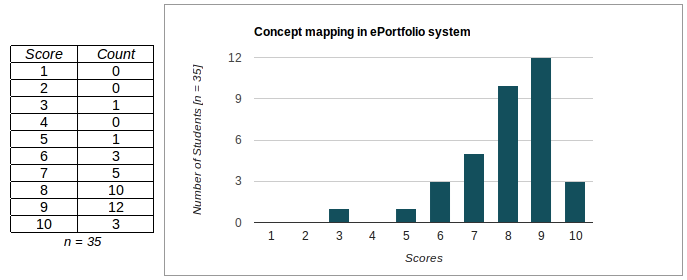
\includegraphics[width=1\textwidth]{CH7-F1-Chart}
\caption{Overall views on usefulness of the used tools and methods}
\label{fig:overall}
\end{figure}

The questions that can be asked here is whether participants' previous
experience with either \ep s systems or familiarity with the \LLLs concepts
influenced the perception of usefulness of the concept mapping tool as a part of
the \ep~system.

For this purpose, the results were split into three groups (Figure
\ref{fig:groups}) based on the differences in participants' experience
reported in the background section (Section A) of the exit questionnaire:

\begin{figure}[htb]
\centering
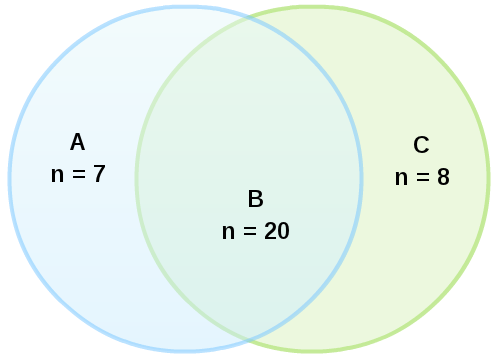
\includegraphics[width=0.6\textwidth]{CH7-F6-Groups}
\caption{Experiment groups based on student profiles}
\label{fig:groups}
\end{figure}

\FloatBarrier

\textit{Group A} represents participants who were familiar with the concepts of
\LLLs prior to the experiment. \textit{Group C} consists of students who have
not been using any kind of \ep~system to demonstrate their \LLLs prior to the
experiment. \textit{Group B} represents an intersection of groups A and C and
therefore consists of students familiar with \LLLsn, but who have not been using
\ep~systems. In this case, \textit{Group A} also represents students who
have used an \ep~system for \LLLs purposes prior to the experiment. Variable
\textit{n} represents a number of participants in each group respectively.

According to such distribution of the participants into groups, the views on
usefulness of the \ep~system concept mapping tools were following:

\begin{figure}[htb]
\centering
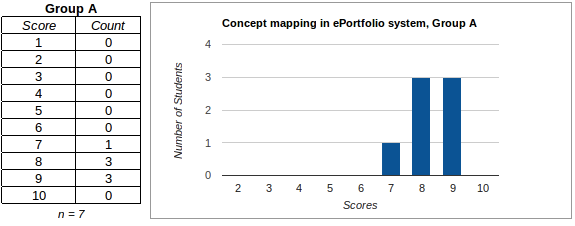
\includegraphics[width=1\textwidth]{CH7-F2-Chart-GA}
\caption{Group A views on usefulness of the used tools and methods}
\label{fig:group1}
\end{figure}

\begin{figure}[htb]
\centering
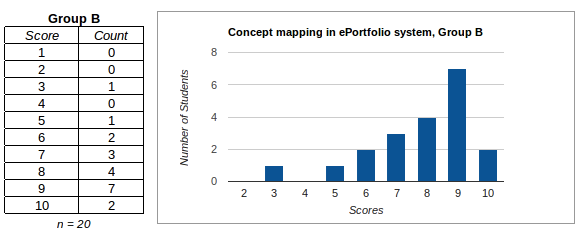
\includegraphics[width=1\textwidth]{CH7-F3-Chart-GB}
\caption{Group B views on usefulness of the used tools and methods}
\label{fig:group2}
\end{figure}

The student from Group B (Figure \ref{fig:group2}) who gave three points to the
usefulness score of the used tools decided not to justify their choice by the
exit questionnaire responses. The only comment they left was \textit{``You can't
quite do what you want with it''} without an overall experience description,
recommended improvements, or description of the least favoured parts.

\begin{figure}[htb]
\centering
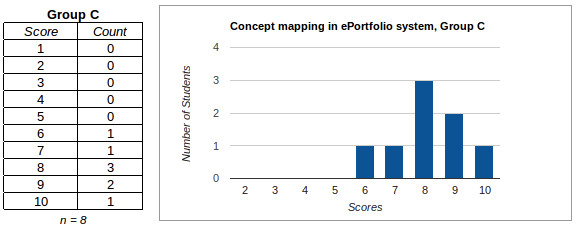
\includegraphics[width=1\textwidth]{CH7-F4-Chart-GC}
\caption{Group C views on usefulness of the used tools and methods}
\label{fig:group3}
\end{figure}

\FloatBarrier

In general, it can be seen that participants of all groups gave high scores as a
measure of usefulness of the concept mapping tools in the \ep~system they had
used. It can be also concluded that the previous experience with the overall
concepts did not have substantial influence on the score distribution. However,
it must be noticed that Group B (Figure \ref{fig:group2}) has a significantly
larger number of students compared to Groups A (Figure \ref{fig:group1}) and C
(Figure \ref{fig:group3}). Nevertheless, the conclusion drawn from this analysis
can be that the novice users find the tools and methods that had been used
during the experiment the same useful as the students familiar with either one
or both concepts of \LLLs and \ep s.

\subsubsection{Concept Maps Created by Students in the \ep~System}

As was requested by the exercise task, the majority of students transferred
their hand drawn concept maps to the \ep~system prototype. A small number of
concepts had the examples attached to them that would demonstrate students'
experience of the related concepts. Due to the fact that the participants had
not been expected to bring any examples with them to the study, they were asked
to think about what examples they would include and create empty files or short
blog posts for these. As was explained to the students, understanding and
evaluation of the general concept rather than content they create was in focus
of this study.

Figure \ref{fig:stdmap} demonstrates the examples of the graduate attributes
maps created by the students using the prototype concept mapping feature during
the experiment. On average, the concept maps developed by the participants were
too large to be includes as a full size illustration. Therefore, this figure
shows the small fragments of such concept maps.

\begin{figure}[htb]
\centering
\setlength\fboxsep{0pt}
\setlength\fboxrule{0.5pt}
\subfigure[Example 1]{
\fbox{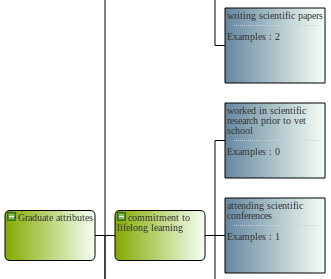
\includegraphics[width=0.47\textwidth]{CH7-F10-ExampleStud1}}
\label{fig:subfig1}
}
\subfigure[Example 2]{
\fbox{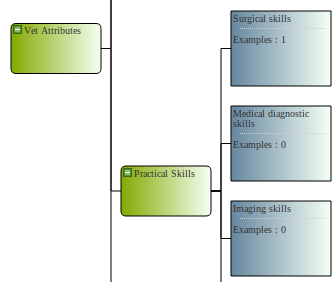
\includegraphics[width=0.47\textwidth]{CH7-F10-ExampleStud2}}
\label{fig:subfig2}
}
\caption{Fragments of the concept maps created by the participants}
\label{fig:stdmap}
\end{figure}

\FloatBarrier

Figure \ref{fig:stdmap2} illustrates an example provided by one of the
participants for the concept they had created.

\begin{figure}[htb]
\centering
\setlength\fboxsep{0pt}
\setlength\fboxrule{0.5pt}
\fbox{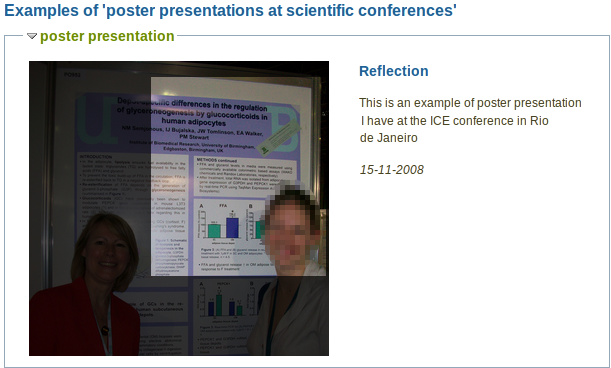
\includegraphics[width=0.8\textwidth]{CH7-F10-ExampleStud3}}
\caption{A concept example provided by one of the participants}
\label{fig:stdmap2}
\end{figure}

Section \ref{sec:examples1} of Appendix \ref{cha:app6} provides more complete
examples of the concept maps created by the students using \ep~tools during the
experiment.

\subsection{Conclusions}

Overall, it can be concluded that the fundamental goal of this study to
evaluate whether the students find prototype tools helpful was accomplished. It
showed that students perception of the concept mapping as a part of the
\ep~system was positive and it provided a suitable means of addressing graduate
attributes and \LLLs skills.

Students who have had prior experience with using the \ep~system to demonstrate
their \LLLs skills said that concept mapping was a great idea and worked better
for them than the \ep~tools they had used before.

Although, usability was not in focus of the prototype requirements, a large
number of students noticed that concept mapping was easy and straightforward to
use. In contrast, extracting fragments of the artifacts and adding them as
examples to the concepts was more complicated and less intuitive task and
required detailed instructions. However, a common agreement among the
participants was that with proper training and experience all tasks can be
easily performed on daily basis.

A problem with the participants testing software rather than evaluating the
overall method and its concepts was expected to be a potential threat to
validity of the outcomes of this study. For this reason, in the introduction
part of the experiment it was emphasized that the participants were going to use
prototype version of functionality and therefore should not pay attention to
the flaws of the user interface, but focus on the process and an overall idea.
Unfortunately, it was impossible to avoid the responses that indicated that
participants were looking at the software and its functionality instead trying
to understand what stands behind it. This could be seen in such comments like
\textit{``Date format on the page is not right for New Zealand''}, \textit{``I
would like to have a choice of color boxes''}, or \textit{``Bigger, more
approachable toolbar would be nice''}. However, there were no more than four
responses similar to these for each question. These responses can be considered
useful in further improvements of the prototype features user interface.

Among the improvements suggested by the participants were:

\begin{itemize}
  \item Simplification of the process of linking examples to the concepts;
  \item Improved maps formatting and reorganizing options for higher
  flexibility of the concepts and better delivery of owners message;
  \item Video tutorial and more detailed instructions on using concept mapping
  tools to ensure that even novice users can start on their own without external
  help;
  \item Options of linking items outside of the \ep~repository to bring other
  sources of learning to the \ep~system;
  \item More examples of the concept maps for students with various profiles --
  resembles the need of providing the students with a model \ep~example.
\end{itemize}

These recommendations can be used to design further improvements to the process
and the overall concept to ensure that they are accepted by the students with
diverse level of experience.
 
\section{Study Three. System Validation by Experienced Students}
\label{sec:three}

The third study in the series of evaluation studies for this research project
investigates whether the prototype features can be successfully employed by the
mature students to provide support for their \LLLs while not being guided by the
lecturer or institutional requirements. This evaluation consists of a series of
case studies which explore the processes and methods used in the \ep~system
prototype with postgraduate students to determine their opinion.

Case studies are commonly used as evaluation method \citep{Yin2012}. The role of
a \textit{case} in the classic case studies is usually played by individuals
\citep{Yin2009}. However, the unit of analysis can be any entity other than a
single individual: case studies can be done about events, programs, processes,
organizations, etc \citep{Yin2009,Patton2002}. The unit of analysis for these
case studies was a prototype of the \ep~system that provided support for \LLLs
in universities.

\subsection{Goals}

The goal for this study was:

\shortquote{To investigate how new features can help students track their
learning progress, manage \ep~knowledge and content, demonstrate and share their
achievements with others.}

To support achievement of this goal, the main objectives were:

\begin{itemize}
  \item To investigate how useful the students find the prototype features for
  the purposes they have been created for;
  \item To explore what are advantages and disadvantages of the implementations
  compared to the other \ep~features which the students have used before;
  \item To demonstrate how the new features can be used by the students for:
  \begin{itemize}
    \item developing understanding of their personal and professional 
    development;
    \item effectively managing their \ep~knowledge and content;
    \item sharing their achievements with others;
    \item communication and getting feedback;
    \item tracking own learning progress; 
  \end{itemize}
\end{itemize}

\subsection{The Case Studies and Participant Profiles}

This study was of exploratory nature and used a multiple case study approach as
an instrument of the evaluation. Although, case studies are known for their poor
generalisation (external validity) \citep{Stake1995}, this problem can be
addressed using the strategies described further in this section.

People, places and times are identified by \citet{Trochim2001} as three major
threats to external validity. To overcome these threats and improve external
validity, he suggests to do the study in \textit{a variety of places, with
different people, and at different times} [p.~43]. Due to the unit of analysis
being a prototype system, place for the case studies in this research was not
relevant. 

On the other hand, time of the case studies would potentially matter as each of
the participants was a student and therefore might have depended on the
university semester schedule. In case of Study Three, all participants were
postgraduate students who had their own research project schedule independent of
the university semester. Therefore, due to no major schedule constraints for
participating in this study, time of conducting the study was considered not
relevant as well. 

This study used a mixture of sampling methods to identify the suitable
participants. First, a criterion sampling method was applied which identified
potential cases who met the general criteria of being a postgraduate mature
student and being familiar with the concepts of \LLLs and \ep.

Then, a \textit{maximum variation (heterogeneity) cases} strategy of purposeful
sampling \citep{Flyvbjerg2006,Patton2002} was applied to narrow down the sample
to three cases. According to this strategy, cases have to be different in at
least one dimension (e.g., experience with using \ep~system, participant's age,
area or program of study) to gather information about influence of various
circumstances on processes and outcomes of the case study. This strategy also
follows the recommendation of \citet{Stake1995} according to which researchers
should try to keep balance between the uniqueness and the ordinariness in the
process of case selection.

In summary, the three case studies were carried out with the mature students who
varied in the areas of study and had different experience of using \ep~systems.

\begin{table}[htb] \small
\setlength{\abovecaptionskip}{0pt}
\caption{Study Three participants profile (n = 3)}
\begin{center}
	\begin{tabular} {| p{3.5cm} | c | c | c |}
	 \hline
	 \multicolumn{1}{|c|}{\textbf{Characteristics}} &
     \multicolumn{1}{c|}{\textbf{Participant One}} & 
     \multicolumn{1}{c|}{\textbf{Participant Two}} & 
     \multicolumn{1}{c|}{\textbf{Participant Three}} \\ \hline
	    Native English speaker & yes & yes & no \\ \hline
	    Age & over 30 & 20-30 & over 30 \\ \hline
	    Degree of study & Masters & PhD & PhD \\ \hline
	    Area of study & Arts & Computer Science & Education \\ \hline
	    Aware of \LLLs & yes & yes & yes \\ \hline
	    Self-rated \ep~use experience (1-10) & 8 & 6 & 8 \\ \hline
	    \multirow{3}{4cm}{Specialized \ep~systems used before}  & 
	    \multirow{3}{*}{MyPortfolio} & \multirow{3}{*}{OSP}  & OSP \\ 
	    & & & The Johns Hopkins DP \\ \hline 
	    \multirow{4}{4cm}{Purpose of previous \ep~use} & Assessment & Research
	    project & Personal development \\ 
	    & C.V. & C.V. & Research project \\ 
	    & Repository & Personal progress & \\
	    & Teaching Aid & & \\ \hline 
	    Currently maintaining \ep & yes & yes & no, but would like to \\
	    \hline
	\end{tabular}
\end{center}
\label{tab:study3part}
\end{table}

Table \ref{tab:study3part} shows the background characteristics of the three
participants. As can be seen, together these characteristics were different
from each other enough to address the issues of poor generalization property of
the case studies as recommended by \citet{Flyvbjerg2006}. At the time of the
evaluation, all three participants were pursuing postgraduate study degrees in
various areas. Apart from being familiar with the \LLLs concepts, this was the
only common characteristics between all three participants.

A self-rated experience of using \ep~systems was relatively similar through all
cases with two participants rating themselves as experienced and one rating as
above average based on scale from one to ten.

Participant One had the longest experience of continually using \ep~system for
various purposes: evidence of personal and professional development, repository
of artifacts, and assessment. As well, they had experience of training others to
use the \ep~system to demonstrate their professional development. At the time of
study, Participant One reported maintaining both personal and professional \ep.

Participant Two with above average experience of using the \ep~systems reported
that they had started using a specialized \ep~system a while back before the
study, but due to personal preferences had returned to their own ways of 
maintaining \ep~through the personal web-site. According to their opinion, this
option provided them with more flexibility and independence from the
institutionally supported, but also limited environments.

Participant Three, while having been actively involved with the \ep~systems
development in their past research carrier, was not maintaining personal \ep~at
the time of evaluation due to the lack of time. As they explained during the
discussion, it was also partly because they could not find a suitable \ep~system
which would provide high-quality free services.

\subsection{Research Protocol}

The study was split into two sessions held in separate meetings with each of
the participants. The main strategy for this study was to give the participants
access to the \ep~prototype environment for a certain period of time so that
they could try the new features on their own and in their own time.

The first session was an introductory meeting and was conducted to familiarize
the participants with the environment they were going to evaluate. Before
starting any study activity, each participant was provided with the information
sheet which stated their rights and the consent form to sign in case they agree
to participate under the conditions outlined in the information sheet. None of
the students had objections to the study conditions.

After all ethics arrangements were finished, the researcher gave a brief
presentation on the research project and the aim of the study. Participants were
demonstrated each implemented feature that was in focus of the evaluation,
explained its purpose and given the examples of potential use. Unlike in the
experiment of the Study Two, in this study, the participants did not have
exercises to complete or tasks to follow. Instead, they were given freedom to
choose what activities to perform given a set of prototype features to evaluate.
Each of the students had an access to the user manual for the features they were
trying out. 

For the evaluation time, the \ep~system prototype was available 24 hours a day
and could be accessed from outside of the university network. This was done so
that the students could work with the system from home and did not depend on
being in the university. To access the features of the system, each student had
to create their personal account which they had to use till the end of the
evaluation period.

All participants were told that the researcher would regularly check on their
progress. As well, they were suggested to contact the researcher any time they
required assistance or when they were ready to discuss the implementations they
had used.

All students were given time to work with the \ep~system prototype until the end
of the calendar year when the evaluation stage was scheduled to finish. This
arrangement would have given each of the participants on average four months of
trial period. Participants Two and Three contacted the researched in less than
one months to schedule the second meeting. Participant One took one and a half
months get back to the researcher with their feedback.

The second session was a discussion meeting organized with each of the
participants after they had finished their evaluations of the prototype. During
the meeting they discussed the ways they employed the new features and how
helpful these features were for the purpose. One of the participants showed
what they had done and during the demonstration pointed out the problems they
had while working with the system. Where possible, each student was asked to
describe advantages and disadvantages of the new features compared to the
\ep~features they had used before. Lastly, they were offered to recommend any
future improvements.

Discussion with each participant took on average 90 minutes and was audio
recorded for the purposes of transcribing and analysis. At the end of the
meeting, the participants were asked to complete a background questionnaire and
provide any other comments that might be valuable for the research evaluations.

According to the participants' requests, they retained their access to the
prototype system after the meeting for the duration of this research project.

The research protocol, examples of potential questions for the discussions, the
background questionnaire, and all other documents related to the Study Three can
be found in Appendix \ref{cha:app7}.

\subsection{Data Analysis and Results}

Each of the case studies utilized multiple sources for data collection:
background questionnaires, semi-structured as well informal discussions, records
made by the participants in the \ep~system, uploaded artifacts, and system logs.

While the participants had access to the evaluated \ep~system, it was possible
to track their system usage: how many times they logged into the system, what
resources they uploaded, and what kind of records they created. However, this
information did not provide the evidence of how long was spent by each of the
participants working with the evaluated features. In this case, the researcher
had to rely on what the participants said at the second meeting.

Based on the system logs, Table \ref{tab:study3stats} shows statistics of the
\ep~system usage by the participants:

\begin{table}[htb] \small
\setlength{\abovecaptionskip}{0pt}
\caption{The prototype usage statistics}
\begin{center}
	\begin{tabular} {| p{3.5cm} | c | c | c |}
	 \hline
	 \multicolumn{1}{|c|}{} &
     \multicolumn{1}{c|}{\textbf{Participant One}} & 
     \multicolumn{1}{c|}{\textbf{Participant Two}} & 
     \multicolumn{1}{c|}{\textbf{Participant Three}} \\ \hline
	    Length of access\footnotemark[1] & 37 days & 7 days & 15 days \\ \hline 
	    No. of logins & 4 & 6 & 5 \\ \hline 
	    No. of records created & 29 & 58 & 23 \\ \hline
	    No. of files uploaded & 8 & 6 & 4 \\ \hline
	\end{tabular}
\end{center}
\label{tab:study3stats}
\end{table}
\footnotetext[1]{Calculated based on the difference between account registration
date and last access date}

During the second session, the researcher discussed system usage log information
with the participants. According on their opinion, all participants considered
that they had had sufficient time to explore the features. 

In general, according to their feedback, all participants viewed the prototype
implementations positively. At the end of the meeting, one of the students said:
\textit{``I've seen a lot of interesting ideas in this system and I would like
to see them moving to the new version of the \ep~system.''}. This can be
interpreted as one of the indicators of success of the \ep~system prototype with
the representatives of the mature student audience.

To take a closer look at the results of the evaluations, each feature is
described further in this section as it was discussed with the students during
the meeting. Direct quotes were taken from the audio recordings transcripts.
Examples of the features usage are the snapshots from the students' system
account.

\subsubsection{Concept Mapping Module}

Participant One called the concept map module as \textit{a really good visual
way to navigate around the entire \ep.} One of the drawbacks of concept mapping
as described by Participant One was that they found it difficult or almost
impossible to make complex concept maps. However, this limitation was due to the
prototype level of implementations rather than shortcomings of the underlying
concept. Participant One liked the idea of concept mapping as a part of the
\ep~system. Although, they said that it should be expected that, as the users
become more confident with the system, they would want to build more complex
links between concepts which is not possible at the moment.

Participant One admitted that they used the concept mapping feature and other
features that were connected to it more than they used anything else in the
prototype. They considered the idea of using concept maps for content and
knowledge management as very promising, but it should be taken to another more
complex level:

\shortquote{Participant One: An interesting idea would be to to be able to
aggregate anything that is added to \ep~by\ldots let's say, tags. For example, I
tag the blog post with this concept tag, and next time I open concept map, I can
see it linked to that concept. I really would like the concept maps to
practically build themselves.}

When the researcher noticed that in this case the idea of meaningful linking of
items in the \ep~system might be lost, Participant One agreed that there should
be a balance between the things that are done automatically and the things that
user would have to do manually.

\begin{figure}[htb]
\centering
\setlength\fboxsep{0pt}
\setlength\fboxrule{0.5pt}
\fbox{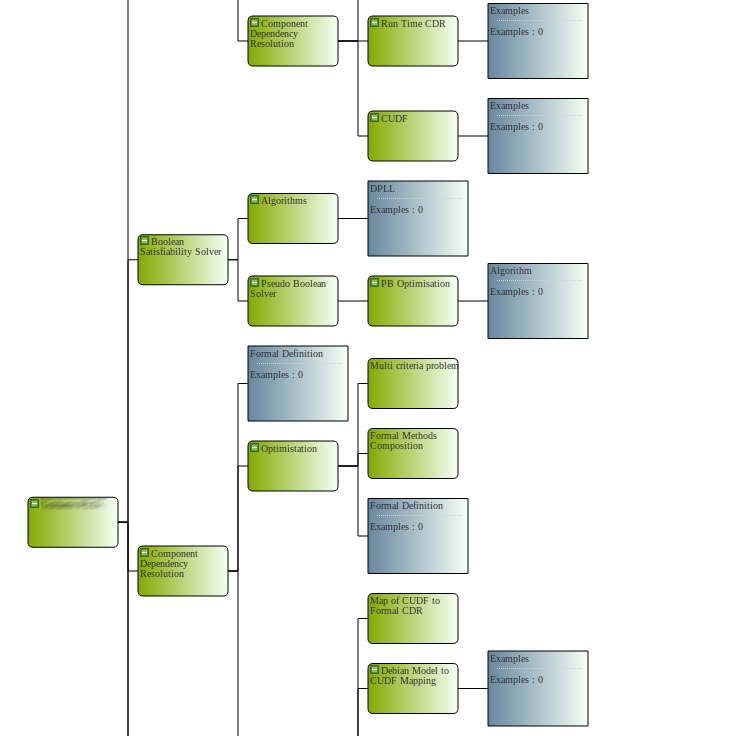
\includegraphics[width=0.9\textwidth]{CH7-F9-Example1}}
\caption{A fragment of a complex concept map created by Participant Two}
\label{fig:p2map}
\end{figure}

As shown on Figure \ref{fig:p2map}, Participant Two used concept mapping to
organize knowledge accumulated and concepts learnt during their PhD studies.
They said that using the tool for this purpose helped them to understand what
has been already done and what would still have to be done in the future.

Participant Two who had prior experience of using rubrics matrix in another
\ep~system as a way of addressing \LLLs skills said that they found the concept
mapping in this \ep~system as much more intuitive knowledge visualization tool
and a tool for demonstration of understanding and achieving objectives.

Participant Two said that \ep~concept mapping was an \textit{excellent tool},
though it required some further improvements of visual personalization. The main
benefit of the feature for Participant Two was in organising and connecting the
various threads that had been learnt. 

\shortquote{Participant Two: It helps to organise and also display the current
progress and review different ideas easily. I feel if the graduate attributes
were there and the students gave examples of these attributes, it would make it
easier to see why certain things were learnt.}

Participant Three found that the idea of adding concept maps to the \ep~system
was \textit{very nice}. They had the long-term prior experience of using concept
mapping technique as a teaching aid at school. Participant Three thought that
linking concepts was particularly good principle in \ep~when learners could
create connection between things they had done.

Participant Three also said that concept maps were user-friendly and their
layout was as well easy for reading. However, similarly to Participant Two, they
suggested that concept maps need more formatting options. While it was not a
major improvement, it would add another level of personalization:

\shortquote{Participant Three: There is a lot of visual learning going on
nowadays. Different learners have different ways of seeing things and being able
to change\ldots shape things according to their views is important if we want to
have an \ep~that is really personal.}

Among the suggestions for improvements to formatting of the concept maps
named by Participant Three were:
\begin{itemize}
  \item Adding labels to the links between concepts;
  \item Color choice for concepts;
  \item Change of orientation of the maps;
  \item Concepts sorting within the maps;
  \item Reorganizing the concepts inside the map.
\end{itemize}

To justify these suggestions, Participant Three explained:

\shortquote{Participant Three: Although, I think the best way to read maps is
when they are laid out like in the prototype, sometimes people just want to try
out how it would look like another way. It might be useful to have an option of
organizing concepts in the maps in their own way.}

Overall, from the feedback given by all participants it can be concluded that
concept mapping as a part of the \ep~system was accepted as a valuable tool to
organizing \ep~knowledge, navigating through the \ep~concepts, demonstrating
achievements of learning objectives, and evaluating of personal learning
progress.

\subsubsection{Artifacts' Fragments Extraction}

Being an Art's student highly involved in design and visual arts, Participant
One was particularly interested in this feature. They said that it would be an
easy way of emphasizing fragments of a visual work and drawing attention of
others to the particular elements of the displayed artifact.

\shortquote{Participant One: The idea of fragments is really interesting. I
haven't seen it in the \ep~systems before.}

Participant Two liked the idea of fragments in terms of viewing a single
document from different perspectives to see what concepts had been learnt. They
said that this feature could be used for splitting up artifacts into different
examples to be presented in the concept map.

From the perspective of their professional field, Participant Two understood the
difficulties of marking up or selecting fragments of the documents that had
proprietary format. However, they said that there could be an choice for users
to open a document as a plain text file for fragment selection. Users generally
know whether their document can be opened in plan text format. This would be
very useful for the students in technical areas, such as Participant's Two,
where a lot of skills are demonstrated in programming and code samples.

Participant Three said that fragments of the artifacts might have a potential
value of communicating ideas more clearly between a learner and a teacher.
From this perspective, selecting an exact part of a picture or limiting a long
video to just a number of time frames allows to be more specific about the
things that students might want to share.

Compared to other \ep~systems, Participant Three liked that reflection could be
directly attached to a potential evidence of any concept from a concept map.
They said that it should be useful for students to be able to explain what and
why they added to their \ep.

It can be concluded that all three participants understood the general principle
of working with this feature. Each of them saw the various ways of applying it
together with the other prototype features in the \ep~system for better
reflection, sharing and emphasizing elements of one's learning that contribute
to the bigger picture of personal development.

\subsubsection{Learning Progress Tracking}

Each of the participants had a common view that timeline-based progress tracking
feature was useful for discovering gaps in their learning and demonstrating
improvements towards achievement of their learning goals. For example,
Participant one said:

\shortquote{Participant One: The timeline is really useful actually in the way
that I can get a really quick look at my progress and re-factor my gaps.}

\begin{figure}[htb]
\centering
\setlength\fboxsep{0pt}
\setlength\fboxrule{0.5pt}
\fbox{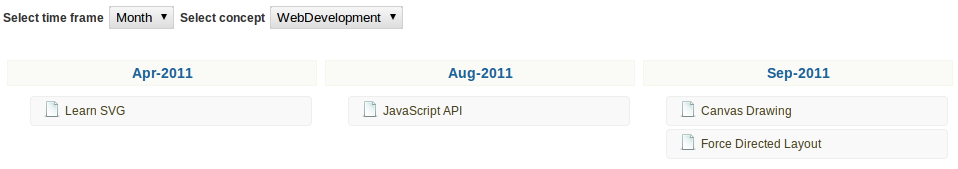
\includegraphics[width=1\textwidth]{CH7-F11-Example3}}
\caption{Progress tracking example by Participant Two}
\label{fig:p2timeline}
\end{figure}

Figure \ref{fig:p2timeline} shows one of the examples of using progress tracking
feature provided by Participant Two. According to them, the timeline
functionality was an \textit{excellent way of viewing progress} which allowed to
see achievements of the past and learning potential for the future:

\shortquote{Participant Two: It enables the view of what I have done and then I
can also see areas for improvement.}

Participant Two did not like the way custom time-frames were supposed to be
created by the users. They found the implementations to be confusing and not
straightforward, although the overall idea looked interesting to them. They
suggested that this part would either require more detailed explanation to the
learners who are just starting to use the \ep~system or considerable changes to
the way custom timelines and time-frames are created.

Participant Three thought that together with the concept mapping tools timeline
provided another perspective on learning. According to their opinion, if used
properly, these features could be a very powerful tool for lecturers to perform
assessment.

\shortquote{Participant Three: In the concept map, someone can see how I
understand the knowledge concepts, while in timeline I can easily show what I
have actually done to address these concepts [\ldots] If I was teaching now, I
would definitely use it with my students.}

Participant One noticed that this feature did not require any manual input from
the users. Although, timeline representation builds itself from the concepts and
examples that learners provide in adjacent features, there might be a room for
data manipulation on timeline level as well. For example, students should be
able to drag examples between time frames which would allow them to easily
update date of an example. Another potential improvements would be a color
highlight of the elements on timeline based on the examples association with a
concept.

Overall, all participants were satisfied with the feature and said that they
could see it working for the purpose of learning progress tracking for students
as well as for lecturers.

\subsubsection{Version Control Elements}

Version control feature was implemented through a simple page versioning in the
\ep~repository. Participant Two really liked the idea of adding this kind of
functionality to the \ep~system.

\shortquote{Participant Two: Everything in \ep~should be done with versions. It
might be my Computer Science background, but for me it's a really good way of
own seeing progress in work.}

According to Participant's Three views, in addition to being able to show the
changes that had been done in the process of developing a showcase \ep~page,
this feature would also help to support discussion between a learner and other
interested parties. An opportunity to justify the changes and communicate the
improvements is a valuable addition to the conventional \ep~systems'
functionality.

\shortquote{Participant Three: I think adding version control elements to the
\ep~system is an excellent idea. It would be useful in many circumstances to
view changes and improvement.}

Participant One said that in the way it is implemented now, \textit{the
lecturers might enjoy this feature much more than students}. As they explained,
traditionally version control features were used for an opportunity to go
back and revert the changes rather than review the progress made between
versions. In case of this implementation, it was more like a version release of
a software when one can introduce improvements and share them with others.
Participant One could not imagine going back and trying to compare versions of
pages, but from the perspective of a lecture, their dialog with a student
that could be supported this way, and an opportunity to review students'
progress, it seemed to be useful.

It can be concluded that all three participants found this feature useful for
the purpose it was created. None of the students could not think of any other
potential applications than the ones suggested by the researcher.

\subsubsection{Shared Resources Management}

Due to the system being a prototype with no social activity going on, none of
the participants could properly test the all features implemented for the shared
resources management. Participant One found the way out by registering another
account and sharing resources between the two accounts. Other participants
followed the descriptions in the user manual and looked at the feature's set ups
without actually sharing resources with anyone. In some cases, they tried out
giving feedback to their own artifacts and other items, or sharing resourced
with the friends group and logged-in users.

Participant Two said that it might be difficult to measure the effectiveness
of the shared items management by just sharing something with others or
compiling a C.V. for a potential employer. According to their point of view, the
problem with this approach would be that there were already effective mechanisms
in place that allowed sharing resources. However, the valuable benefit of this
feature in the \ep~system prototype would potentially be in combination with the
version control feature in order to manage changes and feedback to the artifacts
at the same time.

Participant One noticed that notifications about access to the shared resources
in the \ep~system might not be positively accepted by some users. From the
perspective of people outside of the \ep~community, such notifications might
turn the \ep~system into another spam sending web-site. From their point of
view, this feature required much more options to consider for both a sender and
a person who would receive notifications.

Although, none of the students could evaluate full potential of this feature,
they all said that they could see it being helpful combined with other features
for \LLLs support. However, from the research perspective, these assumptions
have to be tested by further investigations.

\subsection{Conclusions}

Overall, based on the evidence gathered during the case studies, it can be
concluded that all three participants supported the prototype implementations
and agreed that being properly utilized these implementations could be a part of
a successful approach to \LLLs support in universities.

Although, all three participants were generally satisfied with the
implementations, they also tended to suggest a number of improvements for each
feature. These included the following:

\begin{itemize}
  \item improvements to the concept mapping tool for better interaction,
  flexibility and user control;
  \item improvements to the artifacts' fragment extraction to provide users with
  more file options and better communicating their ideas;
  \item improvements to the shared resources management with more opportunities
  for a sender as well as a recipient; 
  \item improvements to the progress tracking using more intuitive creating of
  custom timeline and time-frames;
  \item improvements to the version control feature with more \ep~artifacts
  having version property.
\end{itemize}

Due to some of the tested features' dependence on the social interactions
between the users, it was not possible to evaluate the entire prototype in depth
as it would be necessary before launching the system into the real world
settings. Evaluation according to the thoroughly designed scenarios of potential
use with a larger number of participants would decide strengths and weaknesses
of the implementations performance and feasibility of their use in the social
settings. This can be one of the questions for the future research.

\section{Summary}

This section presented the evaluation design and the results of the evaluation
of this research project's contributions. Three studies were carried out to
understand how the new features can be utilized by the stakeholders to provide
better support for \LLLs in the universities.

The results of these studies can be summarized as follows:

\begin{enumerate}
  \item Lecturers see the ways and are willing to incorporate the new features
  into their teaching to provide students with their guidance and help them to
  understand \LLLs skills.
  \item Based on the experiment results, concept mapping as a part of the
  \ep~system can be successfully used by students to demonstrate learning
  achievements and address institutional graduate attributes. It also can
  provide opportunities for targeted reflection and better feedback.
  \item According to the case studies, students see the new features as
  helpful and useful for tracking their learning progress, managing
  \ep~knowledge and content, demonstrating and sharing their achievements with
  others. Further improvements are still required to make the features more
  flexible, intuitive and user-friendly. This would also ensure that the
  evaluation of the underlying concepts have not been affected by the limits of
  implementations.
\end{enumerate} 

An apparent issue of the evaluation was in the fact that it was very difficult
for some of the participants to give their opinion of the underlying concepts
without paying attention to the shortcomings of the user interface. The
evaluated system was a functional prototype and therefore was not aiming at
providing highly attractive and usable user interface. However, this problem
should be considered and addressed in any future research.
 
\chapter{Discussion\label{cha:discussion}}
%2325
This chapter aims to bring together the knowledge developed during this research
project. It looks back at the topics discussed earlier in the thesis in order to
understand various aspects: whether the research questions were answered; what
issues were faced in the course of this project and how they could be avoided in
future research; what are the implications of this research for theory and
practice; and how the knowledge can be applied in real world.

\section{Answers to Research Questions}

The overall research goals in this thesis was stated as follows:

\shortquote{\textbf{To design and implement a learner-centered e-learning
environment which will support and facilitate the \LLLs process in
universities.}}

To support achievement of this goal, four research questions were developed
(Chapter \ref{cha:method}) and systematically addressed throughout this thesis.
The answers to these questions are summarized in this section.

\shortquote{RQ1. What is the concept of \LLLs and its connection to universities?}

According to the reviews of the area described in Chapter \ref{cha:litrev}, it
can be concluded that the concept of \LLLs is not simple. Lifelong learning
went through various changes in concept as well as in meaning. Even now,
there are debates about what the actual meaning of \LLLs is. The term employed
in this thesis follows the common understanding of the theories where \LLLs
consists of formal, informal and non-formal types of  earning with long-term,
life-wide and self-directed characteristics. This concept puts the learner in
charge of learning and moves educational providers -- universities in the
context of this thesis -- to the role of learning facilitators.

So, what do universities have to do with \LLLs anyway? Looking from tertiary
education perspective, time spent on studying in the universities takes about
5\% of all learning done by an average individual over their life span
(calculated based on statistics provided by Dench
\citeyearpar[28-37]{Dench2010}). While this might not look like too much, a
university is still considered to be a place where professionals are prepared to
join the world of global economics. As a result, the pressure on the university
to produce highly qualified graduates is high. Current economics demands these
graduates to possess not only their specific professional skills, but also
skills that are called \LLLs and are less likely to be developed by just
learning in the classroom. This is where the need of incorporating other types
of learning in addition to formal learning in the universities comes from.
Currently, the universities are looking into ways of providing students with
better support that would reflect their needs as lifelong learners. One of the
types of such support is providing a proper learning environment.

\shortquote{RQ2. How are available e-tools used to support \LLLs within the
university context?}

Exploring the area of learning spaces (Chapter \ref{cha:systudy}) shows that
the field of ICT currently provides a large number of systems and tools
available for supporting all types of learning. Some of these tools are provided
by educational institutions while others are freely available online on the
Internet. All of them have their benefit for various types of learning. However,
the gaps that exist between these tools are difficult to bridge. While LMS
dominates in the world of institutional spaces and provides support for formal
learning according to the university standards, the Web 2.0 tools with their
high potential of supporting informal learning are almost completely neglected
by the universities due to various reasons.

\ep~systems coming to the stage of learning brings an opportunity to cover these
gaps. Although, the \ep~system are developed to provide a highly demanded
support for \LLLsn, it is difficult to measure its success in doing so. The
field of \ep~systems development is still young and therefore rapidly changing.

This research came about very timely, when a lot of studies from the first
\ep~systems' adoption waves were finished and needed understanding of what went
wrong and how the discovered problems can be solved \citep{Batson2010}. Taking
their experience and adding new knowledge to the existing grounds might bring
better theories that would change and improve the ways this technology could be
adopted and used in the future.

\shortquote{RQ3. How can LMS and/or \ep~systems be extended to support students
in the university context for \LLLsn?}

An investigation through a series of interviews with the stakeholders resulted
in development of requirements for better support of \LLLs on a system level
(Chapter \ref{cha:model}). Providing support from LMS perspective was abandoned
at that point as improvement of the \ep~system was considered more important.
High priority requirements were translated into features (Section
\ref{sec:elicit}) and implemented in a system prototype as described in Chapter
\ref{cha:prototype}.

Looking back at the requirements development stage, it would be valid to ask
whether the information gathered was enough to answer the posed question.
Participants selection procedure showed that the pool of potential participants
with suitable experiences was very small. No information was found in related
software engineering literature that would say how many stakeholders was enough
to start developing requirements. Therefore, the researcher followed common
sense by examining the results of the interviews to understand whether data
saturation had been reached.

In addition, the elicitation of the requirements was conducted under the
assumption that the stakeholders involved in this research were competent enough
to provide high quality information that could be used later. All lecturers were
experienced in their field of teaching and had practice of utilizing the
\ep~system in their work with students. In turn, the students they recommended
for participation in this project were all mature individuals with experience of
using \ep~systems in their learning. Measuring the stakeholders expertise or
maturity would go far beyond the scope of this project. Notwithstanding, this
should be considered as an underlying assumption behind this research stage.

\shortquote{RQ4. How does this extended environment meet the needs of
stakeholders in university teaching and learning contexts?}

Evaluation stage of this research, as described in Chapter \ref{cha:evaluation},
attempted to catch various perspectives of the stakeholders by developing a
complex evaluation design that incorporated three studies, each using different
evaluation approach. Through these studies it was shown that the representatives
of all of the stakeholders were largely satisfied with the implementations in
the \ep~system prototype. Therefore, it can be concluded that in general their
requirements were met.

Arguably, artificial settings of all studies might have influenced the general
reliability of the outcomes of this evaluation. This stage was conducted
under the assumption that the conditions of the evaluations would resemble those
of the real world situations. Taking into account that the evaluated system was
a functional prototype and could not be launched into the real worlds setting,
it was a reasonable trade between getting high quality evaluation results
against getting no results at all. As was required, additional measures were
undertaken to increase validity of the overall evaluation. However, the results
of the evaluations have to be accepted with understanding the conditions and
assumptions of the studies.

\section{Implications For Theory and Practice}

This section discusses the lessons learnt and conclusions that can be drawn
based on results of this research. It suggests the changes that could be made in
various areas in order to improve the quality of \LLLs support in universities.

\subsection[Cooperation and Communication]{Work directed towards introducing
new technologies or new teaching principles should be done in cooperation}

A surprising discovery made during the course of this research was that
communication between various departments was poor. If the lecturers were
familiar with the research carried out in their departments or schools, they
were less likely to know about similar research projects in other areas of
the university. Work with the lecturers at various stages of this project showed
the importantce of communication and cooperation between the universty
departments. The lecturers who were research participants were usually highly
surprised when they discovered that some other departments were using or had
past experience of employing exactly the same technologies with their students.
A lot of issues and troubles could have been avoided if proper communication or
presenting departments' research was done across the university.

\subsection[Finding Balance]{Finding balance between what is good for teaching
and good for learning}

For lecturers it might be difficult to find a balance in what should be used for
teaching and learning. This research confirmed a known fact that different
people have different perspectives. For lecturers it is especially important as
they have to look at things not from only their own teaching perspective, but as
well from the perspective of learners. It was easy to notice that some of the
participants had difficulty with understanding learners' needs due to not being
able to put themselves into their students' place.

On the other hand, it would not be a reasonable decision to ask lecturers to
employ technologies that might significantly adversly affect their established
teaching process. For example, changing the way lecturers give material to
students or the way they mark learners' assignments might increase the time that
has to be spent on these activities to get quality outcomes. Therefore, while
introducing new systems to the learning environment, university management
should also make sure that it would be possible for the lecturers to find this
kind of balance without harm to learning and teaching process.

\subsection[Learning to Use Technology]{Using new technology needs to be learnt
as any other things around}

A curious fact was noticed in the course of this research: the students who
participated in various studies of this project had practically no complaints
about LMS used in their university, although LMS and the \ep~systems were
discussed equally. In contrast, the \ep~system raised criticism and expressions
of dissatisfaction. How is it that the system that has been built for learners
displeases these very learners so much? There is a number of possible
explanations for this. Some of them are discussed here. Others are explored in
the following section.

Universities usually offer a number of supporting courses for students on how to
use the institutional systems. Unfortunately, the \ep~system is not on the list
of such systems. One of the lecturer-participants of this research noticed that
using the \ep~system should be taught to students the same way as any other
system. However, currently, in best case students get a number of video tutorials
or manual web-pages on the \ep~system use. These were shown to be insufficient. 

\ep~trials, and this research is not an exception, are rarely carried out with
the students who are recent high school graduates. There is a number of reasons
for this: students who have already studied at the university for some time are
more familiar with the requirements for the systems, better understand the needs
and can provide their opinion comparing with their own previous experience.

However, looking from different perspective might draw another picture. While
studying at the university, students are developing their own expectations and
experiences of using various systems. In this case, if the \ep~system is
introduced at the later stages of a study program, students who have never been
taught the value of reflection, purposeful selection of artifacts and
demonstration of personal achievements might not see the value of the \ep~system
as well. Starting their learning journey with the \ep~system rather than trying
to fit \ep~into the students' usual way of learning might result in more
positive outcomes and lead to higher acceptance of the \ep~concepts and systems
among the students. Although, this assumption needs to be carefully tested in
the future.

\subsection[Shaping Technology for Learning Needs]{Learning theory and practice
should shape the way technology is developed, not the other way around}

Following the discussion in the previous section, the reality of nowadays is
such that technology is shaping the way learning and teaching are performed. It
is not unusual for the university to employ the new technology without
understanding the needs of learners, but simply because it offers higher degree
of security and regulation as well as more opportunities for control and
management. An approach that is driven by the needs of the university rather
than the learner cannot have much potential from the learner's perspective. This
research attempted to take into account this perspective placing a learner, a
student in this context, and their needs first.

Unlike in business settings where a consumer usually dictates the software
features that are being developed, students generally do not have such influence
on technology which they have to use. This means that very often learning
technology is being developed separately from its main stakeholder -- a learner.
As a result, such technology is more likely to reflect developers' understanding
of the problem rather than users'. One of the recommendations based on the
explorations of the area of this project is to create an environment where
systems for learning are being built in cooperation with learners and teaching
experts. Listening to users' needs first and the needs of finances and
management second is very important for successful outcomes of any project. This
would ensure that the developed technology created for learning is accepted  by
its intended consumers -- the learners.

\section{Applications}

The results of this research can be applied in many areas and domains. Among
these can be education, employment and workplace, knowledge and information
management, media sharing, etc. The principles and implementations of this
research can be used for providing support for various learning processes in the
universities, such as developing understanding of skills and learning concepts,
demonstrating achievements, assessment of knowledge, and others. This was shown
by a number of evaluation studies described in Chapter \ref{cha:evaluation}.

Formal requirements specification for \LLLs support developed in the course of
this project (Chapters \ref{cha:model} and \ref{cha:prototype}) can be used by
the \ep~systems' developers to add new features and functionality to the
existing systems with the aim of improving learners' experience. This
specification can also be used as a guiding specification in requirements
management of the new system development.

To support the applicability of this research, with additional improvements
and necessary corrections its implementations could be added to the official
release of Mahara \ep~system -- the system used as a basic \ep~system for
prototyping. This \ep~system is getting more popularity in New Zealand with an
expectation of providing \LLLs support for every New Zealand citizen.
 
\chapter{Conclusions and Future Work\label{cha:conclusion}}
\epigraph{We now accept the fact that learning is a lifelong process of keeping
abreast of change. And the most pressing task is to teach people how to
learn.}{\textit{Peter F. Drucker}}

The main focus of this thesis has been on improving \LLLs support for students
in the universities by providing them with better learning environment -- an
enhanced \ep~system. For this purpose, the requirements, design, development and
evaluation of the prototype environment has been discussed in detail. This final
chapter summarizes the main contributions of this research to the related
fields, along with the opportunities for the future research projects.

\section{Research Contributions}

Text

Discovering the requirements for the \LLLs in the universities

Development of the functional prototype

\section{Future Research}

Text

\section{General Conclusions}

Text 
 
% ========================Appendices================================
%\appendix
%\chapter{Ethics Documentation: Requirements Analysis}

This appendix provides the ethics documentation used in the study of \LLLs
requirements described in Chapter \ref{cha:model}. The following documents are:

\begin{itemize}
  \item Letter of ethical approval for the study.
  \item Information sheet for lecturers.
  \item Information sheet for students.
  \item Participant Consent form.
\end{itemize}


\includepdf[scale=0.7,pages=1,pagecommand=\section{Ethics Approval
Letter},frame]{appendix/Low-Risk-Notification-2009.pdf}


\includepdf[scale=0.7,pages=1,pagecommand=\section{Information Sheet for
Lecturers},frame]{appendix/Lecturer_sheet_1.pdf}
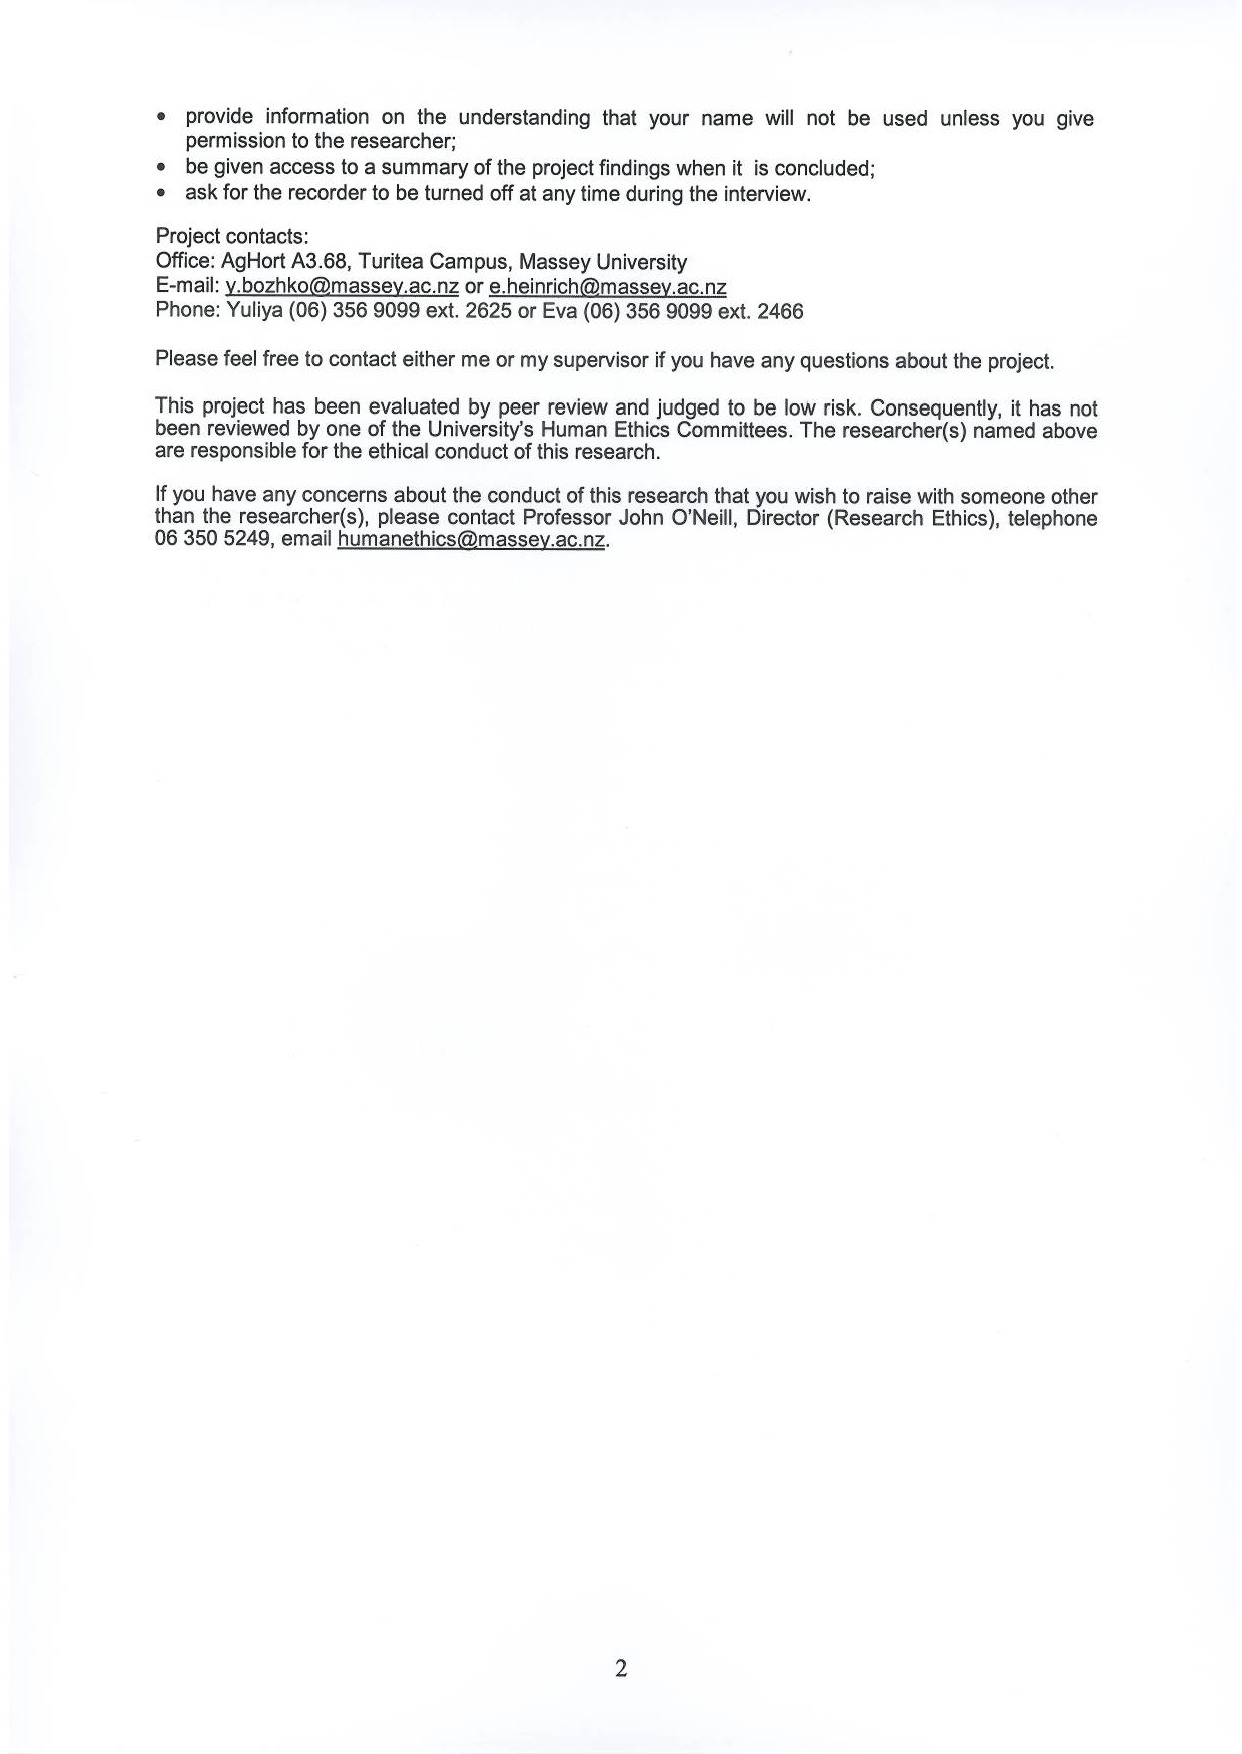
\includepdf[scale=0.7,pages=1,pagecommand={},frame]{appendix/Lecturer_sheet_2.pdf}


\includepdf[scale=0.7,pages=1,pagecommand=\section{Information Sheet for
Students},frame]{appendix/Student_sheet_1.pdf}
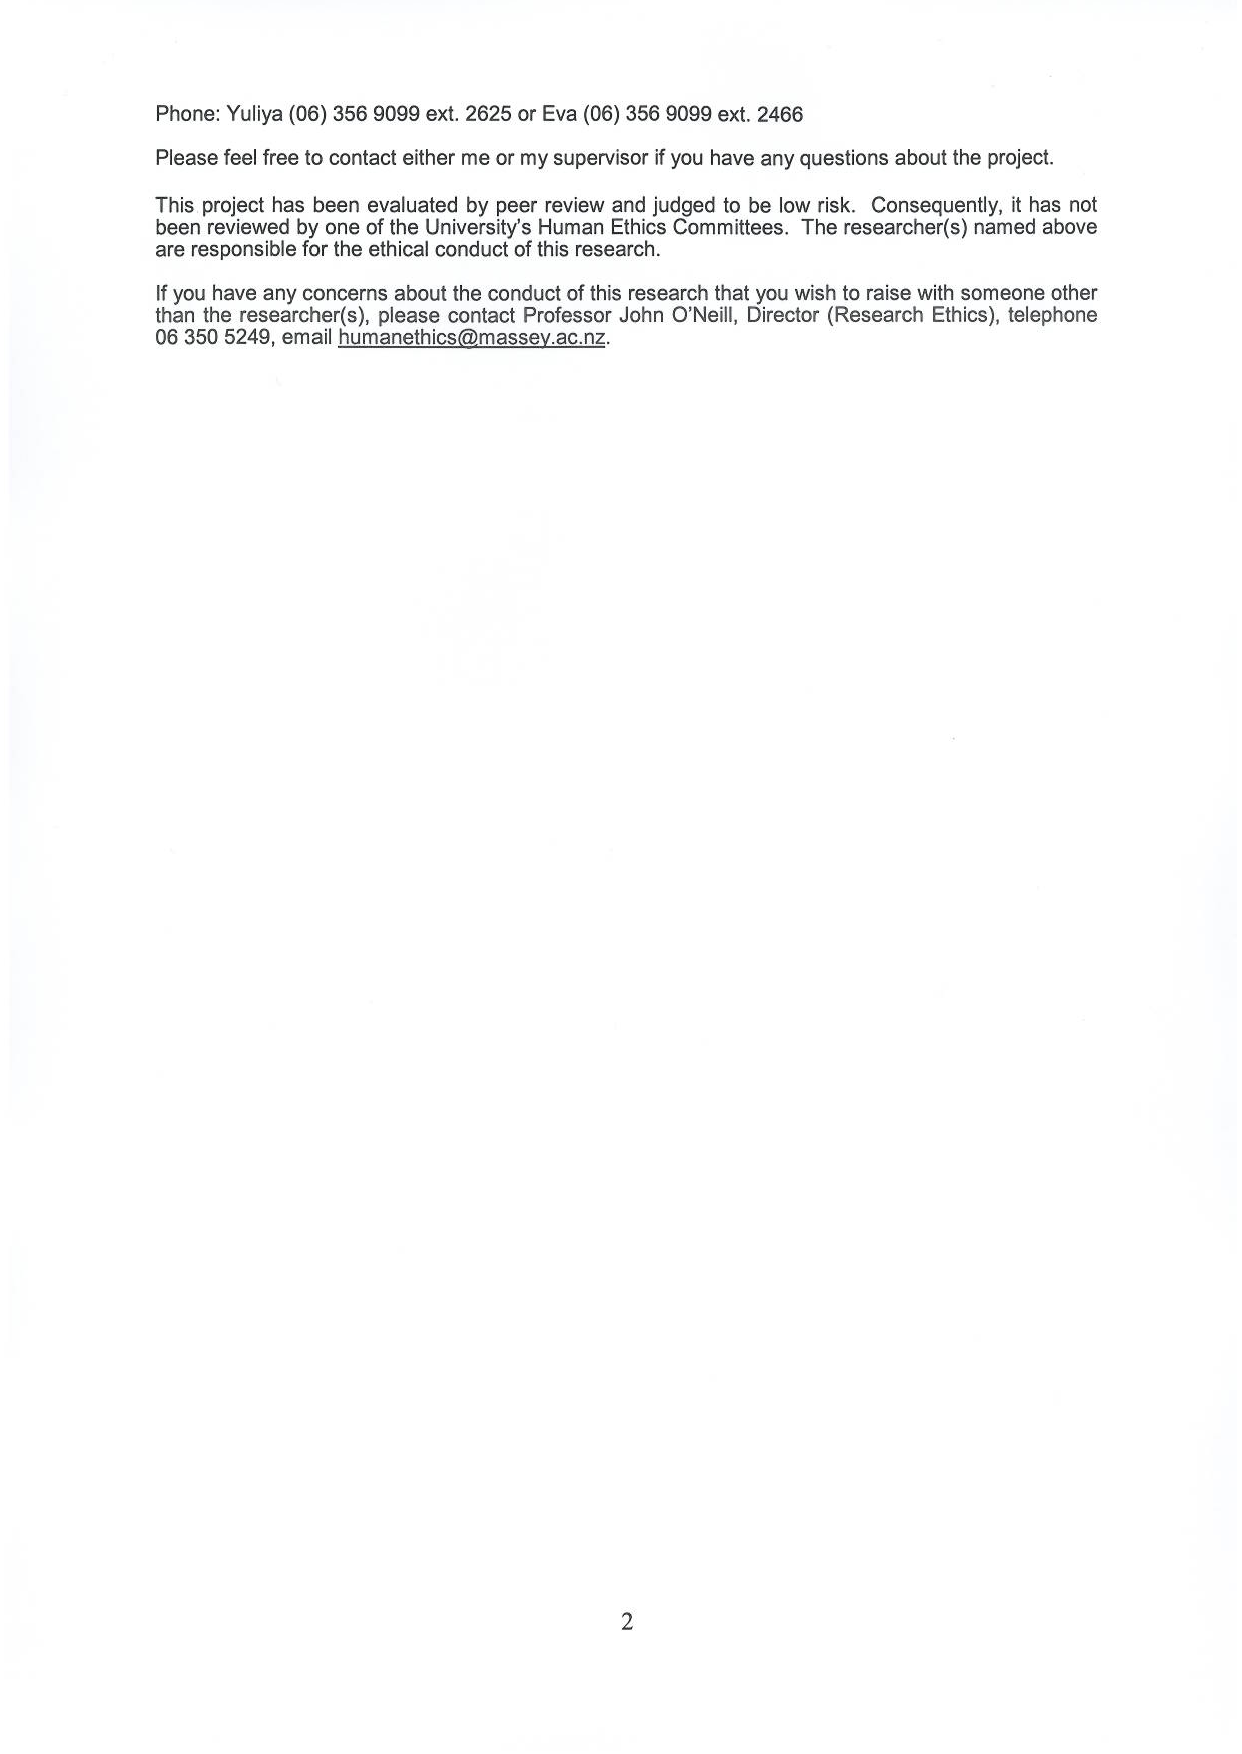
\includepdf[scale=0.7,pages=1,pagecommand={},frame]{appendix/Student_sheet_2.pdf}

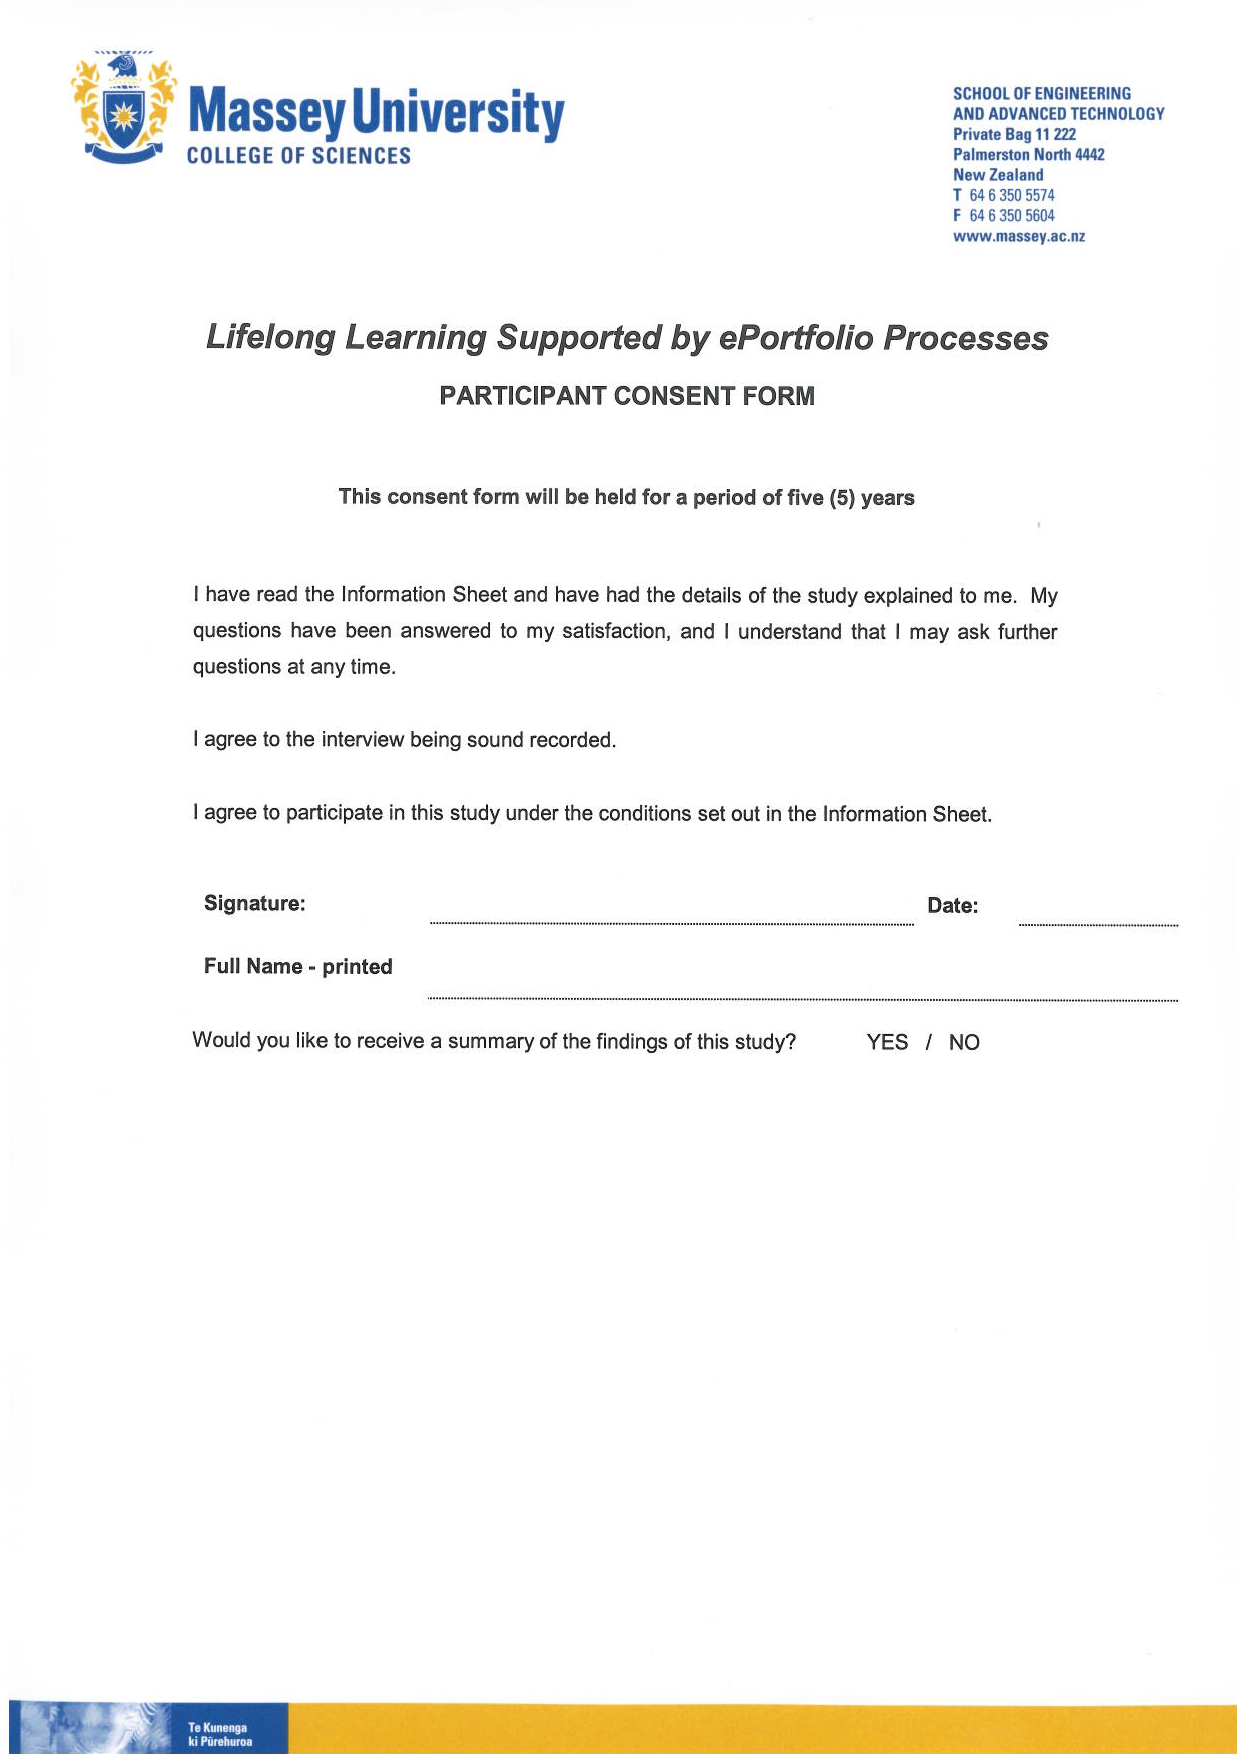
\includepdf[scale=0.7,pages=1,pagecommand=\section{Participant Consent
Form},frame]{appendix/Consent_form.pdf}

%\chapter{Interviews Documentation}

\section{Questions used in the interviews}

\section{Scenario examples}

% ========================Bibliography==============================

\addcontentsline{toc}{chapter}{Bibliography}
\bibliography{references}             
\bibliographystyle{bevbib4}%{plainnat}  

\end{document}
